
% Header reference level
\clearpairofpagestyles
\chead{\headmark}
\automark[subsection]{subsection}
\ifoot{\ifootertext}
\ofoot{\ofootertext}
\cfoot{\thepage}

\section{Coding Guidelines}
\label{sec:CodingGuidelines}

% Header reference level
\clearpairofpagestyles
\chead{\headmark}
\automark[subsection]{subsection}
\ifoot{\ifootertext}
\ofoot{\ofootertext}
\cfoot{\thepage}

In this section, we provide guidelines for coding institutional statements at the IG Core, IG Extended, and IG Logico Levels of Expressiveness. Following the specification of utilized syntax, we specify encoding principles for regulative and constitutive statements.

\subsection{Coding Symbols \& Syntax}
\label{subsec:CodingSyntax}

\subsubsection{Coding Symbols}
\label{subsubsec:CodingSymbols}

The syntactic coding for examples in the remainder of this document relies on specific symbols, whose function depends on the applied context, i.e., grammar component vs. institutional statement, and respective coding level (IG Core, IG Extended, IG Logico). An overview of all symbols along with application context, minimum level of applicable encoding, description and examples is provided in \cref{tab:SymbolReference}. The specific syntactic notation referenced in this codebook (introduced in \citep{Frantz2022InstitutionalGrammar}) is referred to as \begin{emp}IG Script\end{emp}\footnote{A more detailed discussion of all syntactic features of IG Script are provided under \url{https://github.com/chrfrantz/IG-Parser?tab=readme-ov-file\#ig-script}.}, a notation that manages the trade-off between computational representation on the one hand, and retaining general human readability of the encoded text on the other. Before exploring the encoding in practice more generally, initially all commonly referenced symbols are introduced, alongside specific features that are applicable in particular levels of expressiveness.

Throughout the remainder of this section we use color coding to signal the association/introduction of specific symbols for syntactic components or features with specific levels of expressiveness (as introduced in  \cref{subsec:IgCodingLevels}). Symbols associated with IG Core features are held in \textcolor{\corecolor}{\corecolorname} for regulative statements, and in \textcolor{\corecolorconst}{\corecolorconstname} for constitutive statements (specifically relevant from \cref{tab:CodingIgCoreConstitutive} onward). Symbols associated with IG Extended are held in \textcolor{\extendedcolor}{\extendedcolorname}, and features associated with IG Logico are called out in \textcolor{\logicocolor}{\logicocolorname}. Symbols of general relevance across levels and regulative and constitutive statements (e.g., parentheses to signal precedence or nesting) are held in bold \textbf{black}. Naturally, the examples draw on features not introduced to this stage, but offer an illustration of the representations used throughout the subsequent guidelines. 

\begin{longtable}{p{1.5cm} p{2cm} p{2.2cm} p{4cm} p{4.5cm}}
\toprule
\textbf{Symbol/ Symbol Pairs} & 
\textbf{Coding Context} & 
\textbf{Lowest applicable Level of Expressiveness} \& \textbf{Statement Type} & 
\textbf{Description} & 
\textbf{Example} \\
\midrule
\lp~~\rp & 
Component & 
IG Core, Regulative \& Constitutive Statements & 
Component classification: The characterization of an expression as a component type is signaled through parentheses that contain the component type. & 
\begin{exi}\A{}(Certifier) \dots\end{exi} , where \A{}~identifies the \begin{exi}certifier\end{exi} as an attribute in a given institutional statement. \\
 & 
 & 
 &
\\
 &
 &
 &
 Where used to combine individual components of the same type (in addition to annotation or the indication of statement combinations), parentheses signal component-level combinations (with logical operators discussed at the end of this table). Inner parentheses are only needed to indicate precedence for three or more elements linked by different logical operators. &
 \begin{exi}Attendees must not \I{}\lp eat \AND{}~drink\rp~on the train.\end{exi}

 
 Note that this is equivalent to `Attendees must not \I{}(\lp eat \AND{}~drink\rp)~on the train.', but the additional parentheses can be omitted, unless relevant to indicate precedence (e.g., combinations of three or more actions with differing logical operators), such as \I{}\lp firstAction \AND{}~\lp secondAction \OR{}~thirdAction\rp \rp.
 \\
\midrule
 \textit{[}~~\textit{]} & 
 Component & 
 IG Core, Regulative \& Constitutive Statements & 
 Tacit components: The explicit specification of implied components (e.g., actor(s)) is signaled with brackets. & 
 \begin{exi}They [\A{}(farmers)] must comply with the certification regulation \dots, where [\A{}(farmers)] characterizes the inferred actor.\end{exi} \\
 & 
 & 
 &
 \\
 {[~~]} &
 &
 &
 Where component annotations (e.g., animate, inanimate) are used, those are embedded in square brackets following the component symbol, but preceding the component content. & 
 \begin{exi}\A{}\customLog{type=animate}(Certifier) \dots\end{exi}, where \A{}~identifies the \begin{exi}certifier\end{exi} as an attribute in a given institutional statement, and \begin{exi}animate\end{exi} as a semantic annotation, a feature of specific relevance in IG Extended (applied in \cref{subsubsec:IGExtendedRegulative}) and IG Logico (from \cref{subsubsec:IGLogicoRegulative} onward).\\
\midrule
\{~~\} & 
Statement & 
IG Core, Regulative \& Constitutive Statements & 
Horizontally nested statements are represented using surrounding parentheses to emphasise the precedence of combined individual statements. & 
\begin{exi}\{ stmt \AND~stmt \}; \{ stmt \AND~\{ stmt \OR~stmt \}\}\end{exi}, where stmt represents an institutional statement combined with other institutional statements using logical operators (\AND, \OR, \XOR, and potentially \NOT) -- more details on logical operators below. \\
& 
& 
&
&
\\
&
&
&
Vertically nested statements are represented using braces that embed the respective consequential statement & 
\begin{exi}stmt1\{stmt2\}\end{exi}, where \begin{emp}stmt1\end{emp} represents a monitored statement, and \begin{emp}stmt2\end{emp} the corresponding consequential statement. \\
\midrule
\lb~~\rb & 
Component & 
IG Extended, Regulative \& Constitutive Statements & 
Component-level nesting is represented by embedding the component-substituting nested institutional statement in braces. In the case of component-level nesting, the component type specification follows the embedded nested statement. & 
\begin{exi}\A{}(Certifier) \I{}(believes) \Bdir{}\lb \A{}(farmer) \I{}(violates) \Bdir{}(code of conduct)\rb\end{exi} 

\vspace{0.5cm}
 In this example, the direct object (\Bdir{}) of a given institutional statement is substituted with another institutional statement. \\
\midrule
 \A{} & 
 Component & 
 IG Core, Regulative Statements & 
 Identifies the preceding expression as Attributes component.[2] & \begin{exi}\A{}(Certifier)\end{exi} \\
\midrule
 \I & 
 Component & 
 IG Core, Regulative Statements & 
 Identifies the preceding expression as aim component. & 
 \begin{exi}\A{}(Certifier) \I{}(monitors) \Bdir{}(farmers).\end{exi} \\
\midrule
 \Bdir{} & 
 Component & 
 IG Core, Regulative Statements & 
 Identifies the preceding expression as direct object component. &
 \begin{exi}\A{}(Certifier) \I{}(administers) \Bdir{}(certifications).\end{exi} \\
\midrule
 \Bind{} & 
 Component & 
 IG Core, Regulative Statements & 
 Identifies the preceding expression as indirect object component. &
 \begin{exi}\A{}(Certifier) \I{}(registers) \Bdir{}(certification) for \Bind{}(organic farmer).\end{exi} \\
%\midrule
% \B{} & 
% Component & 
% IG Extended, Regulative Statements &
% Identifies objects that are neither direct nor indirect, but contained as functionally-independent objects in the institutional statement (see Attributes/Object-Properties Hierarchy in \cref{subsec:AttributeObjectHierarchy}). & 
%\begin{exi}\dots~\Bdir{}(notification) of \Bext{a},\Bext{1}(suspension) or %\Bext{a},\Bext{2}(revocation) of \Bext{a}(certification) \dots\end{exi} \\
%
% & 
% &
% &
% First-order properties are identified by alphabetic identifiers (e.g., \Bext{a}, \Bext{b}, etc.); second-order properties are identified with numeric identifiers (e.g., \Bext{1}, \Bext{2}, etc.). & 
% Here, the functionally independent object \begin{exi}certification (\Bext{a})\end{exi} is root of a property structure consisting of two objects as properties [\begin{exi}suspension  (\Bext{a},\Bext{1}), revocation (\Bext{a},\Bext{2})\end{exi}], both of which are annotated with reference to the certification.\\
\midrule
 \D{} & 
 Component & 
 IG Core, Regulative Statements &
 Identifies the preceding expression as a deontic modal representing duty. &  
 \begin{exi}\A{}(Certifier) \D{}(must) \I{}(monitor) \Bdir{}(farmers).\end{exi}\\

\midrule

\Cac{}/\Cacconst{} & 
Component & 
IG Core, Regulative \& Constitutive Statements & Identifies the preceding expression as an activation condition component. & 
 \udl{Regulative:} \newline
 \begin{exi}\Cac{}(Upon accreditation) \A{}(certifier) \D{}(must) \I{}(monitor) \Bdir{}(farmers).\end{exi}
 \newline \newline \udl{Constitutive:} \newline
 \begin{exi}\Cacconst{}(From 1st January onwards), \E{}(Council) \M{}(shall) \F{}(include) \Pp{}(organic farming representatives) \Cexconst{}(to review chemical allowances within organic food production standards).\end{exi} \\
\midrule

\Cex{}/\Cexconst{} & 
Component & 
IG Core, Regulative \& Constitutive Statements & Identifies the preceding expression as an execution constraint component. & 
\udl{Regulative:} \newline 
\begin{exi}\A{}(Certifier) \D{}(must) \I{}(monitor) \Bdir{}(farmers) \Cex{}(at any time).\end{exi} 
\newline\newline \udl{Constitutive:} \newline 
\begin{exi}\Cacconst{}(From 1st January onwards), \E{}(Council) \M{}(shall) \F{}(include) \Pp{}(organic farming representatives) \Cexconst{}(to review adherence with food production standards).\end{exi} \\

\midrule

\E{} & 
Component & 
IG Core, Constitutive Statements & 
Identifies the preceding expression as constituted entity & 
\begin{exi}\Cacconst{}(From 1st January onwards), \E{}(Council) \M{}(shall) \F{}(include) \Pp{}(organic farming representatives) \Cexconst{}(to review chemical allowances within organic food production standards).\end{exi}\\

\midrule

\Pp{} & 
Component & 
IG Core, Constitutive Statements & 
Identifies the preceding expression as constituting property & 
\begin{exi}\Cacconst{}(From 1st January onwards), \E{}(Council) \M{}(shall) \F{}(include) \Pp{}(organic farming representatives) \Cexconst{}(to review chemical allowances within organic food production standards).\end{exi} \\

\midrule

\F{} & 
Component & 
IG Core, Constitutive Statements & 
Identifies the preceding expression as constitutive function & 
\begin{exi}\Cacconst{}(From 1st January onwards), \E{}(Council) \M{}(shall) \F{}(include) \Pp{}(organic farming representatives) \Cexconst{}(to review allowances within organic food production standards).\end{exi} \\

\midrule

\M{} & 
 Component & 
 IG Core, Constitutive Statements &
 Identifies the preceding expression as a modal representing existential necessity (in contrast to duty or permission in regulative statements). & 
 \begin{exi}\Cacconst{}(From 1st January onwards), \E{}(Council) \M{}(shall) \F{}(be responsible) \Cexconst{}(for adherence with food production standards).\end{exi}
 \newline \newline \udl{Alternative example:} \newline
 \begin{exi}\Cacconst{}(From January 1st onward), there \M{}(shall) \F{}(be) a \E{}(National Organic Standards Advisory Council) \Pp{}(within the Department of Agriculture).\end{exi} \\
 
\midrule

\prop{}/ \propconst{} & 
Attributes, Object, Entity and Property components &
IG Core, Regulative \& Constitutive Statements &
Identifies properties of attributes and objects respective. The \begin{emp}prop\end{emp} symbol is used in conjunction with the respective component identifier. If coding on IG Extended level, where multiple properties for a given component exist, they receive a numeric index suffix. 

\vspace{1.05cm}

IG Extended further supports the explicit encoding of object and property hierarchies.

Where multiple levels of object/properties exist in the property hierarchy, those are contextualized with the objects/properties they refer to (i.e., they are appended to the component specification). Further details on property coding are provided in \cref{tab:CodingIgExtendedRegulative} and illustrated below.

& 

\udl{IG Core:}\newline\newline
\udl{Regulative:}\newline
\begin{exi}\A{},\prop{}(Certified organic) \A{}(farmers) \D{}(must) \I{}(respond) to \Bdir{},\prop{}(formal) \Bdir{}(certification requirements).\end{exi}
\newline\newline
\udl{Constitutive:}\newline
\begin{exi}The \E{}(Council) \F{}(consists of) \Pp,\propconst{}(elected)  \Pp{}(officials) \Pp,\propconst{}(resident in the electorate).\end{exi}
\newline\newline
\udl{IG Extended:}\newline\newline
\udl{Regulative:}\newline
\begin{exi}\A{},\propExt{1}(Certified) \A{},\propExt{2}(organic) \A{}(farmers) \D{}(must) \I{}(respond) to \Bdir,\propExt{1}(formal) \Bdir{}(certification requirements).\end{exi}
\newline\newline
\udl{Constitutive:}\newline
\begin{exi}The \E{}(Council) \F(consists of) \Pp,\propExt{1}(elected) \Pp(officials) \Pp,\propExt{2}(resident in the electorate).\end{exi}

\\
 & 
 & 
 &
 & 
\\

 & 
 &
 &
 &
\\
 &
 &
 &
 &

\\

 \prop{}/ \propconst{} \formatNeutral{(ctd.)}

 & Component
 & IG Extended, Regulative \& Constitutive Statements
 &
 The example on the right highlights a complex object hierarchy structure previously discussed in the context of the Object-Property Hierarchy (\cref{subsec:AttributeObjectHierarchy}). As mentioned above, where multiple objects on a given hierarchy level exist, they are uniquely identified with a numeric index (e.g., \begin{exi}\Bext{1}\end{exi}, \begin{exi}\Bext{2}\end{exi}, etc.). Where multiple properties on a given hierarchy level exist (where properties can be objects by themselves), they are uniquely identified with a numeric index (e.g., \begin{exi}\propExt{1}\end{exi}, \begin{exi}\propExt{2}\end{exi}, etc.). & 
 
 \begin{exi}\dots~\Bext{1},\propExt{1},\propExt{};\Bext{1},\propExt{2},\propExt{}(proposed) \Bext{1},\propExt{1}(suspension) or \Bext{1},\propExt{2}(revocation) of \Bext{1}(certification) \dots\end{exi}
 
 
 \\

 & 
 &
 &
 Where a single property applies to multiple properties, references to both objects/properties are maintained on this property (separated by semicolon). & 
 \\

\midrule

\AND{}, \OR{}, \XOR{}, \NOT{} & 
Statement, Component & 
IG Core, Regulative \& Constitutive Statements &
The logical operators identify the relationship between statement and/or components as either conjunction (\AND{}), inclusive disjunction (\OR{}), or exclusive disjunction (\XOR{}), as well as any combinations thereof. Where negation is involved, the \NOT{}~ operator is used (e.g., in deontics: must not; combination of exceptions: \NOT{}~\lp option 1 \AND{}~option 2\rp). & 
\begin{exi}\A{}(Certifiers) \D{}(must) \I{}\lp review \AND{}~ assess\rp~\Bdir{}(applications).\end{exi} 

\vspace{0.5cm}

\begin{exi}\A{}(Certifiers) \D{}(must) \I{}\lp review \AND{}~ \lp approve \XOR{} reject \rp \rp~\Bdir{}(applications).\end{exi} 

\vspace{0.5cm}

\begin{exi}\A{}(Certifiers) \D{}(must) \NOT{}~\I{}(review) \Bdir{}(applications) by \Bdir,\prop{}(offenders).\end{exi}

\\
\toprule

\caption{Symbol Reference for IG Coding as applied in this document}
\label{tab:SymbolReference}
\end{longtable}

\subsubsection{Coding Syntax}
\label{subsubsec:IGScript}

Following the intuitive introduction of the individual symbols annotating particular features of an institutional statement (e.g., actors, actions), at this stage, we will highlight selected syntactic principles of IG Script more explicitly, since these will be referenced specifically in the more advanced coding examples. The base syntax of IG Script is as follows:

\vspace{0.2cm}
\begin{exa}componentSymbol\lp~\dots~encoded content~\dots~\rp\end{exa}
\vspace{0.2cm}

\dots~where \begin{emp}componentSymbol\end{emp} is a symbolic reference to the component of choice as introduced in the previous \cref{subsubsec:CodingSymbols} (e.g., \begin{exi}\A{}(actor)\end{exi}). 

Where component values are combined as part of horizontal nesting, the linkage and the scope of the linkage is explicitly captured by parentheses (e.g., to indicate elements that apply to both linked values): 

\vspace{0.2cm}
\begin{exa}componentSymbol(shared value \lp left value \ls logicalOperator\rs~right value\rp~shared value)\end{exa}
\vspace{0.2cm}


Applied operationally, this can be exemplified as \begin{exi}\I{}(to \lp revise \AND{}~resubmit\rp )\end{exi}

All relational logical operators can be applied in this fashion, including a nested representation, in which additional parentheses indicate precedence in the case of different logical operators, such as exemplified below:

\vspace{0.2cm}
\begin{exa}\I{}\lp \lp revise \AND{}~resubmit\rp~\OR{}~revoke\rp\end{exa}
\vspace{0.2cm}

For logical operators of the same kind the indication of precedence can be omitted.

\vspace{0.2cm}
\begin{exa}\I{}\lp revise \OR{}~resubmit \OR{}~revoke\rp\end{exa}
\vspace{0.2cm}

The logical operator \NOT{}~plays a particular value, and can annotate individual components as well as statements as a whole.

Taking the following example, 

\begin{exa}
\A{}(Author) \D{}(must \NOT{}) \I{}(review) \Bdir{},\prop{}(own) \Bdir{}(paper).
\end{exa}

the operator can invert a single component value. 

\vspace{0.2cm}

Statements can be scoped using braces (\lb, \rb), e.g., to delimit multiple statements, or to reflect nesting structures. An example for a scope statement is 

\vspace{0.2cm}
\begin{exa}
\lb\A{}(Actor) \D{}(must) \I{}(conform) \Bdir{}(with policy).\rb
\end{exa}
\vspace{0.2cm}

Augmenting this statement with the inversion operator (where of analytical value) leads to the negated interpretation of the statement entirely:

\vspace{0.2cm}
\begin{exa}
\lb\A{}(Actor) \D{}(must) \I{}(conform) \Bdir{}(with policy)  \NOT{}\rb
\end{exa}
\vspace{0.2cm}

A central feature linked to the use of braces is the concept of vertical nesting and component-level nesting, i.e., the substitution of a given component of an institutional statement with the syntactic form of an institutional statement (e.g., preconditions expressed in terms of institutional state characterizations). Where components are augmented with braces instead of parentheses, this signals component-level nesting. 

In the case of vertical nesting, the \ORELSE~ (syntactically represented as \Oe{}) is essentially substituted with an entire statement (identifying the consequences of violating the monitored statement), as shown in the following example:

\vspace{0.2cm}
\begin{exa}
\A{}(citizen) \D{}(must) \I{}(conform) with \Bdir{}(policy) \Oe\lb \A{}(official) \D{}(may) \I{}(sanction) \Bdir{}(citizen)
\Cex{}(immediately)\rb.
\end{exa}
\vspace{0.2cm}

Where nesting occurs on other components, this is annotated in equivalent form. Component-level nesting is commonly found in the context of the activation condition by expressing preconditions for a particular activity in the same structure as the activity itself. This is exemplified in the following: 

\vspace{0.2cm}
\begin{exa}
\A{}(Official) \D{}(must) \I{}(impose) \Bdir{}(fine) \Cac{}\lb \A{}(citizen) \I{}(violates) \Bdir{}(rule)\rb.
\end{exa}
\vspace{0.2cm}

Implied component values are indicated with brackets surrounding the inferred value. For example, the observed statement ``they must comply'' may be contextually interpreted as ``citizens must comply''. To make this inference explicit, it can be encoded as follows:

\vspace{0.2cm}
\begin{exa}
\A{}([citizens]) \D{}(must) \I{}(comply).
\end{exa}
\vspace{0.2cm}

A common observation in the context of complex statements is the unique linkage between particular components and associated properties, an aspect related to the Object-Property Hierarchy (\cref{subsec:AttributeObjectHierarchy}). To indicate the direct linkage, the encoding relies on suffices associated with particular components in order to identify the linkage. 

\vspace{0.2cm}
\begin{exa}
\A{}(Official) \D{}(must) \I{}(impose) \Bdir{1},\prop{}{}(monetary) \Bdir{1}(fine) 

\Cac{}\lb \A{}(citizen) \I{}(violates) \Bdir{}(rule)\rb.
\end{exa}
\vspace{0.2cm}

A feature referenced in the context of IG Logico is the augmentation of the encoded institutional statements with semantic annotations that facilitate epistemological linkages to concepts drawn from theory of interest, or general categorizations introduced as part of the taxonomies discussed in \cref{sec:Taxonomies}. Semantic annotations are captured in squared brackets following the component symbol, but preceding the parentheses scoping the component content specification. The following example showcases the use of semantic annotations:

\vspace{0.2cm}
\begin{exa}
\A{}\customLog{type=actor}(Official) \D{}\customLog{stringency=prescription}(must) \I{}\customLog{act=administer}(impose) 

\Bdir1,\prop{}{}\customLog{prop=quals}(monetary) \Bdir{1}\customLog{object=sanction}(fine).
\end{exa}
\vspace{0.2cm}

Where annotations pertain to the statement entirely, the specification precedes the statement scope as shown below (here exemplified based on the qualification of the statement as regulative):

\vspace{0.2cm}
\begin{exa}
\customLog{regulativeStatement}\lb\A{}\customLog{type=actor}(Official) \D{}\customLog{stringency=prescription}(must) 

\I{}\customLog{act=administer}(impose) \Bdir{1},\prop{}{}\customLog{prop=quals}(monetary) \Bdir{1}\customLog{object=sanction}(fine).\rb
\end{exa}
\vspace{0.2cm}

\subsection{Regulative Statement Coding}
\label{subsec:RegulativeStatementCoding}

The base syntax of regulative statements (as shown in \cref{fig:RegulativeStatementLevels}) consist of necessary (in solid boxes) and sufficient components (in dashed boxes) as defined in \cref{tab:SyntacticElementsRegulative} using the symbols introduced in \cref{tab:SymbolReference}. The figure organizes feature refinements across different levels of expressiveness.

\begin{figure}[h!]
    \centering
    \framedfigure{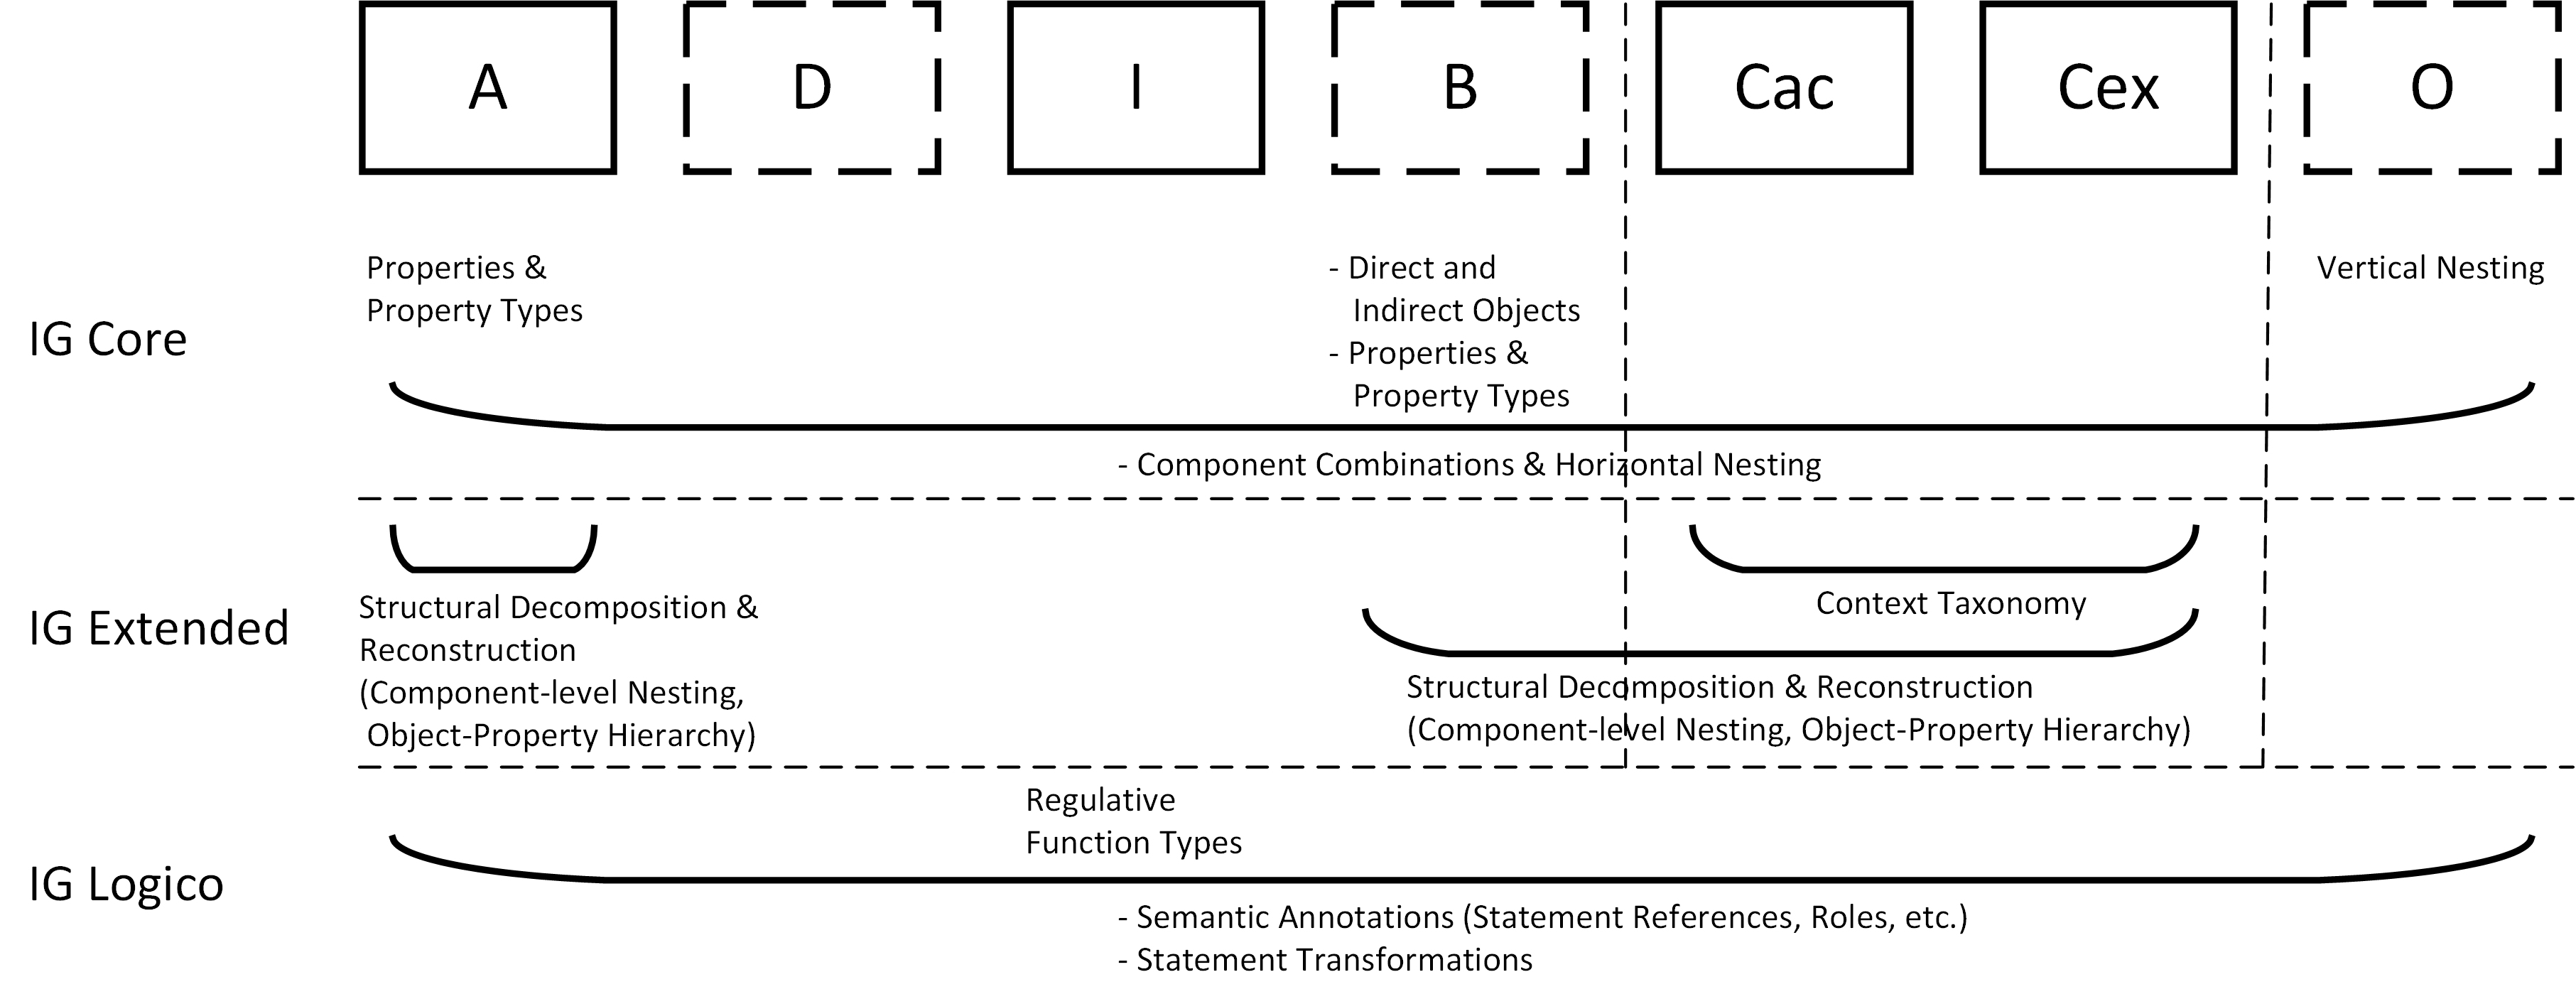
\includegraphics[width=0.95\textwidth]{figures/IGRegulativeLevels.png}}
    \caption{Syntax and Features of Regulative Statements by Level of Expressiveness}
    \label{fig:RegulativeStatementLevels}
\end{figure}

Motivating the principal coding of regulative statements (without further elaboration at this stage), a stylized atomic regulative statement, coded in shorthand form, thus reads: 

\begin{exa}
\A{},\prop{}(Certified) \A{}(farmers) \D{}(must) \Cex{}(strictly) \I{}(adhere) to \Bdir{}(organic farming practices) 

\Cac{}(following their certification).
\end{exa}

\sp

The following Tables \ref{tab:CodingIgCoreRegulative} to \ref{tab:CodingIgLogicoRegulative} provide detailed coding guidelines for regulative statements for all individual components, organized by level of expressiveness, starting with IG Core through IG Logico, leveraging the notation convention captured in \cref{subsec:CodingSyntax}. As the institutional analyst commences coding at any level of expressiveness, the following general coding principles should be entertained.

\begin{itemize}
    \item Where possible, the targeted level of encoding should be clarified at the beginning (see \cref{subsec:IgCodingLevels}).
    \item The coder should acquaint oneself with the concepts relevant for the target level of encoding (see \cref{subsec:IgCodingLevels}), as well as coding conventions, such as applied notation. A specific concern discussed as part of the planning process is the handling of absent syntactic components that are either implied or can be inferred from policy texts.
    \item Recall that coding can (but does not have to) occur iteratively, starting at one level that prompts less granular syntactic expressiveness (e.g., IG Core) moving with a subsequent coding pass to another level that prompts more granular coding (e.g., IG Extended). However, the specific approach is subject to coder experience, and of course available tool support, all of which should be considered in the planning phase (see \cref{sec:PrecodingSteps} for further considerations). 
\end{itemize}

\newpage


\begin{landscape}

\subsubsection{IG Core Coding of Regulative Statements}
\label{subsubsec:IGCoreRegulative}

\begin{longtable}{\tabledims}

\toprule
\multicolumn{4}{l}{\textbf{Level of Expressiveness: IG Core}} \\
\multicolumn{4}{\tablespan}{ 

IG Core enables basic, structural analysis of institutional statements. Encoding at this level is designed to be human readable and moderately comprehensive in the detail with which syntactic properties of institutional statements are captured.} \\

\toprule
{\textbf{Syntactic\newline Component}} & 
{\textbf{Treatment of Syntactic Components by Level of Encoding}} &
{\textbf{Relevant Examples}} &
{\textbf{Complete Syntactic Classification of Examples}} \\
\toprule

%\midrule
\begin{emp}Attributes\end{emp} & {The encoding of Attributes, which can include an animate actor (individual or organizational) only or an animate actor and a property of this actor, differentiates between actor (Attributes) and actor property (Attribute Properties).

\sp

An important decision to establish reliability is a shared understanding of the level of decomposition of Attributes and their corresponding properties performed as part of the coding process (or even pre-coding process), an aspect that relies on the domain, context, and nature of the coded policy. 

The example on the right illustrates the principles of decomposition assuming the most fine-grained possible decomposition. 

Guidelines to determine the appropriate level of decomposition are provided below.

} & 


{\udl{Example statement:} 

\begin{exi}Certified farmer must submit an organic system plan annually. \end{exi}

\sp

\udl{Attributes encoding:}

\sp

Attributes = \begin{exi}certified farmer\end{exi}
 
\sp
 
Actor = \begin{exi}farmer\end{exi}
 
\sp
 
Actor property = \begin{exi}certified\end{exi}
 
} & 

\vspace{0.03cm}

\begin{exi}{\A{},\prop{}(Certified) \A{}(farmer) \D{}(must) \I{}(submit) an \Bdir{}(organic systems plan) \Cex{}(annually). }\end{exi} \\

% Multicolumn overview
\begin{emp}\hypertarget{tablink:AttributePropertyHeuristics}{Attributes (ctd.)}\end{emp} & \multicolumn{3}{p{17cm}}{

\udl{Deciding on the level of decomposition into Attributes and corresponding Attribute Properties:}

\sp

\begin{emp}The guidelines provided below equally apply to Object and Object Properties; Constituted Entity and Constituted Entity Properties; Constituting Properties and Constituting Properties Properties.\end{emp}

\sp

A general challenge across multiple components of the IG is the identification of appropriate heuristics for the decomposition of actor descriptors into Attribute and corresponding properties, and likewise Objects and Object Properties, etc. To support the study design, we propose a set of guidelines to inform the choice of decomposition levels as appropriate for a given study.

\sp

General note: Named entities (e.g., United States Department of Agriculture) are \begin{emp}not\end{emp} decomposed into component properties, i.e., such terms are always annotated as Attributes, Object, Constituted Entity or Constituting Properties, but not their corresponding properties (i.e., Attributes Properties, Object Properties, Constituted Entity Properties, Constituting Properties Properties). 

\sp

Guidelines for determining level of decomposition (in order of consideration):

\begin{itemize}
\item Policy documents often contain a `Definitions' article or section, in which concepts of relevance to the policy are specified. Where this is the case, these definitions represent the desirable level of decomposition, i.e., if `Organic farmer' is defined as part of the definitions, no further decomposition is required, unless analytical objectives motivate further decomposition (see next item).

\item Where absent, the level of decomposition is contingent on the policy focus and context. If, for example, a regulation differentiates between organic and non-organic farmers, the decomposition into descriptor and associated properties is useful, in which both `types' of farmers are distinguished by the properties. If, however, the regulation is exclusively concerned with organic farmers, the decomposition is of little analytical value at this level of encoding.

\item Absent any other guidelines, decomposition should be performed on the most fine-granular level.
\end{itemize}} \\

\newpage

\midrule
\begin{emp}Object\end{emp} & {The encoding of Objects identifies Direct Objects specified within institutional statements, along with their respective properties. Where statements are comprised of both direct and indirect object, it also entails the explicit identification of indirect objects, i.e., objects that are affected by the application of the aim to direct objects, e.g., which the action is targeted to. 

Objects can be concrete or abstract entities. Concrete entities can be animate (e.g., farmers) or inanimate (e.g., notification) in kind. Abstract entities (e.g., beliefs, goals, observations) are generally expressed in terms of statements of facts or institutional statements. The coding of such statements (\begin{emp}component-level nesting\end{emp}) is discussed under IG Extended (see \cref{tab:CodingIgExtendedRegulative}).  

\vspace{0.2cm}

%\newline
Rules:
\begin{itemize}
    \item Identify object identifier
    \item Identify object properties
    \item Repeat for the indirect object
\end{itemize}

\udl{Note:} The separation of Objects and Object properties operates identical to the decomposition of Attributes and Attributes properties. See corresponding guidelines provided under the Attributes component specification (see \hyperlink{tablink:AttributePropertyHeuristics}{here}).} & 

{\udl{Example statement:}

\begin{exi}Organic certifier must send farmer notification of compliance within 30 days of inspection.\end{exi}

\vspace{0.5cm}

{Direct Object = \begin{exi}notification of compliance\end{exi}}

\vspace{0.5cm}

{Indirect Object = \begin{exi}farmer\end{exi}}

\vspace{0.5cm}

{Object property = \begin{exi}organic\end{exi}}

\vspace{0.5cm}

Note: The interpretation of property depends on the encoded policy (and, of course, the coder’s analytical objectives). If a policy on organic farming exclusively refers to organic farmers as a proper noun, organic is not an attribute property, but part of the attribute; if the policy differentiates between organic and other types of farmers, capturing the specific characterisation as property is suggested. For the example here we highlight the second pathway.

} &

{
\vspace{0.03cm}

\begin{exi}\A{},\prop(Organic) \A{}(certifier) \D{}(must) \I{}(send) \Bind{}(farmer) \Bdir{}(notification of compliance) \Cex{}(within thirty days of inspection).\end{exi}} \\

\begin{emp}Object (ctd.)\end{emp} & \multicolumn{3}{p{13cm}}{
\udl{Potential pitfalls:}
\begin{itemize}
     \item \begin{emp}Objects vs.~Constraints\end{emp}: The introduction of the indirect object offers the benefit of capturing the functional interdependence of objects and implied directionality. This directionality is sometimes explicitly reflected, as in the following statement. When encountering such statements, the coder should be careful to not mischaracterize the indirect object preceded by a preposition as context. Example: ``Parents must take children to school.'', ``school'' is sensibly resolved as indirect object, but based on its prepositional embedding, could be mislabeled as constraint. For the characterization, we thus require an initial consideration of clauses containing objects (other than the direct object) as indirect objects, before characterizing those as a contextual descriptor (which primarily make reference to the contextual embedding of actions).

    \item \begin{emp}Object Properties vs.~Constraints\end{emp}: Differentiation between the object property and execution constraint can also sometimes be challenging in the encoding. When such confusion arises, the coder should ask herself to reflect on whether the statement words or clauses in question are qualifying the object or qualifying the action of the statement. Take the following statement for example that illustrates the referenced potential confusion: ``Certifiers shall perform audits on product stock two times per year.'' The clause that may potentially give rise to confusion is ``on product stock.'' This could be confused as an execution constraint relating to purpose, but in fact it describes the type of audit to be performed. \end{itemize}
} \\

\midrule
\begin{emp}Aim\end{emp} & {The encoding identifies the focal action of the statement.} & \udl{Example statement:}

\begin{exi}Organic certifier must send farmer notification of compliance.\end{exi}
\newline

Aim = send
 & 
 
 \vspace{0.03cm}
 
 \begin{exi}{\A{},\prop{}(Organic) \A{}(certifier) \D{}(must)  \I{}(send) \Bind{}(farmer) \Bdir{}(notification of compliance).}\end{exi} \\

\newpage

\midrule

\begin{emp}Deontic\end{emp} & 

{The encoding identifies the prescriptive operator that indicates whether the Aim (i.e., action) of the statement is required, allowed, or forbidden. Common Deontics indicating varying levels of prescriptive force include \begin{emp}must\end{emp}, \begin{emp}may\end{emp}, and \begin{emp}must not\end{emp}.} & 

{\udl{Example statement:}

\begin{exi}Organic certifier must send farmer notification of compliance.\end{exi} 
\newline

Deontic = must
} & 

\vspace{0.03cm}

\begin{exi}{\A{},\prop{}(Organic) \A{}(certifier) \D{}(must) \I{}(send) \Bind{}(farmer) \Bdir{}(notification of compliance).}\end{exi} \\

\midrule
\begin{emp}Context\end{emp} & 
{The encoding identifies the Context of the institutional statement. The encoding differentiates between \begin{emp}``Activation Conditions,''\end{emp} which are contextual clauses that specify preconditions under which the Aim is expected to occur or not occur, and \begin{emp}``Execution Constraints,''\end{emp} which are contextual descriptors that qualify the Aim by assigning in relation to it temporal, spatial, procedural, and/or other constraining parameters.} & 
\udl{Example statement:} 

\begin{exi}Upon entrance into agreement with organic farmer to serve as his/her certifying agent, organic certifier must inspect farmer’s operation within 60 days.\end{exi}

\sp

Context clauses: \begin{exi}Upon entrance into agreement with organic farmer to serve as his/her certifying agent; within 60 days.\end{exi}

Context encoding: 

\sp

Activation Condition: \begin{exi}Upon entrance into agreement with organic farmer to serve as his/her certifying agent\end{exi}

\sp

Execution Constraint: \begin{exi}within 60 days\end{exi}

\sp

Note: While coding the essential aspects of the statement, IG Core is limited with respect to capturing the nested complexity in the activation condition. We will revisit this statement in the context of IG Extended coding.
 & 
{

\vspace{0.03cm}

\begin{exi}\Cac{}(Upon entrance into agreement with organic farmer to serve as his/her certifying agent), \A{}(organic certifier) \D{}(must) \I{}(inspect) \Bdir{}(farmer’s operation) \Cex{}(within 60 days).\end{exi}} \\

\newpage

\midrule

\begin{emp}Or else\end{emp} 

&

The encoding of Or else statements identifies consequences (e.g., payoffs) of compliance/non-compliance with institutional statements, or the conduct of Aim (i.e., activities) assigned to specific Attributes (i.e., actors) in institutional statements. The encoding captures these consequences, which generally  take the form of regulative institutional statements that nest from the ‘non-Or else’ (monitored)  statements.

\sp

Sometimes, the statements on which Or else, or consequential statements, nest convey a combination of  monitoring activity and the associated  payoff attached to outcomes of monitoring actions. 

\sp

The encoding of Or else statements accommodates both vertical and horizontal nesting. Vertical nesting is applicable when there is one payoff activity that is specified within a distinct institutional statement as a consequence of an action indicated in another institutional statement. Horizontal nesting is applicable when there are two or more payoff activities that can be pursued as consequences of an action indicated in another institutional statement. 

&

\udl{Example:} 

\begin{exi}Certified organic farmers must not apply synthetic chemicals to crops at any time once organic certification is conferred, or else certifier will revoke certification from farmer.\end{exi}

\sp

Or else clause comprising statement: \begin{exi}or else certifier will revoke certification from farmer\end{exi}

\sp

Or else statement nests on: \begin{exi}certified organic farmers must not apply synthetic chemicals to crops at any any time once organic certification is conferred\end{exi}

\sp

The above encoding exemplifies vertical nesting. The following example, which is an extension of the above, exemplifies horizontal nesting within a vertically nested statement. 

\sp

\udl{Example statement:} 

\begin{exi}Certified organic farmers must not apply synthetic chemicals to crops at any time once organic certification is conferred, or else certifier will revoke certification from farmer or fine farmer.\end{exi}


& 

In the following example, horizontal nesting is signaled using parentheses (\lp~and \rp) around statements (as opposed to individual components), and vertical nesting is expressed using braces on the \ORELSE~component (\lb~and \rb). 

\sp

\udl{Vertical nesting:}

\begin{exi}\A{},\prop{1}(Certified) \A{},\prop{2}(organic)  \A{}(farmers) \D{}(must not) \I{}(apply) \Bdir{}(synthetic chemicals) to \Bind{}(crops) \Cex{}(at any time) \Cac{}(once organic certification is conferred), \Oe{}\lb  \A{}(certifier) \D{}(will) \I{}(revoke) \Bdir{}(certification) from \Bind{}(farmer)\rb.\end{exi}


\\

\begin{emp}Or else (ctd.)\end{emp}

&

These statement combinations can signal 

\begin{itemize}
    \item alternative exclusive action options -- XORs -- (e.g., either suspending XOR revoking the certification),
    \item inclusive action options -- ORs -- (e.g., sanctions apply if a driver is caught speeding AND/OR on the phone) or 
    \item co occurring action options -- ANDs -- (e.g., fining a transgression AND reporting to authorities).
\end{itemize}

& 

\udl{Or else clauses comprising statements:} 

\begin{exi}or else certifier will fine farmer or revoke certification from farmer.\end{exi}

\sp

\udl{Vertical and horizontal Or else nesting encoding:}

\sp

\begin{exi}Certified organic farmers must not apply synthetic chemicals to crops at any time once organic certification is conferred\end{exi}

\sp

\udl{[Vertical nesting]}

\sp

\begin{exi}or else certifier will revoke certification from farmer\end{exi}

\sp

\udl{[Horizontal nesting]}

\sp

\udl{\XOR~(signaling exclusive or)}

\sp

\begin{exi}Or else certifier will fine farmer\end{exi}

&

\udl{Horizontal nesting within vertically-nested statement:}

\begin{exa}\A{},\prop{1}(Certified) \A{},\prop{2}(organic) \A{}(farmers) \D{}(must not) \I{}(apply) \Bdir{}(synthetic chemicals) to \Bind{}(crops) \Cex{}(at any time) \Cac{}(once organic certification is conferred), 

\Oe{}~\lb\lb \A{}(certifier) \D{}(will) \I{}(revoke) \Bdir{}(certification) from \Bind{}(farmer)\rb~
\XOR~ 
\lb \A{}(certifier) \D{}(will) \I{}(fine) \Bdir{}(farmer)\rb \rb.\end{exa}

\\

&
\multicolumn{3}{p{13cm}}{
\udl{Note:} 
\begin{itemize}
    \item Where component-level combinations exist (\dots~fine farmer \begin{emp}or\end{emp} revoke \dots), those have to be signaled explicitly by parentheses, or be decomposed into separate logically-combined complete atomic institutional statements. Further details are provided under 
    \hyperlink{tablink:DecompositionOfComponentLevelCombinationsExtendedRegulative}{\begin{emp}General IG Extended Instructions\end{emp}, Item \EntryDecompositionOfComponentLevelCombinations} in \cref{tab:CodingIgExtendedRegulative}.
    \item Ambiguities with respect to the linguistic use of logical operators (exclusive and inclusive or) are to be resolved as part of this process. 
\end{itemize}
}
\\

%\midrule

\newpage

\midrule
\multicolumn{4}{l}{\textbf{General IG Core Instructions for Regulative Statements}} \\
\midrule

\begin{emp}Additional annotations for Attributes, Objects, and Context\end{emp}

\sp

(\udl{Note:} This feature is analogous to the specification of additional annotations for Constituted Entity, Constitutive Function and Constituting Properties components in the context of constitutive statements.)

& 
In addition to the identification of properties embedded in the original statements, components can further be annotated using additional annotation labels. Such labels can follow the categories listed in \cref{sec:Taxonomies}, or be specific to the project objectives. 

\sp

A systematic approach to labelling entities is discussed under \hyperlink{tablink:CrossComponentSemanticAnnotationsLogicoRegulative}{\begin{emp}IG Logico Instructions\end{emp}, Item \EntryCrossComponentSemanticAnnotations} in \cref{tab:CodingIgLogicoRegulative}. This is particularly recommended if annotations are of strong relevance for the coding and of diverse nature. 
& 
\udl{Example statement:} 

\begin{exi}Organic certifier must send farmer notification of compliance.\end{exi} 

\sp

Subject to analytical necessity, additional annotations can for instance relate to the identification of aspects such as the characterisation of encoded objects with respect to their animacy as either animate or inanimate -- signified in brackets in the coded example. Where indicated, the annotation should be separated from the component specification by semicolon and have the structure ``\begin{exi}label=\end{exi}'', followed by the annotation. 

Note that ``\begin{exi}label\end{exi}'' is a characterizing prefix, either based on a specific taxonomy (see \cref{sec:Taxonomies} for an overview), or a custom coder-defined category specification (e.g., defined as part of the project-specific guidelines). In this example, the Animacy Taxonomy has the prefix \begin{emp}\anim\end{emp} as defined in \cref{sec:Taxonomies} and is used correspondingly.

\sp

While exemplified here for regulative statements, this equally applies to constitutive statements. 
& 

\vspace{0.03cm}

\begin{exi}\A{}\customLog{\anim=animate}(Organic certifier) \D{}(must) \I{}(send) \Bind{}\customLog{\anim=animate}(farmer) \Bdir{}\customLog{\anim=inanimate}(notification of compliance).\end{exi} \\

\newpage

\midrule

\hypertarget{tablink:DecompositionOfComponentLevelCombinationsCoreRegulative}{\EntryDecompositionOfComponentLevelCombinations} 

\sp

(Note: This applies to regulative and constitutive statements, and is discussed here with focus on the regulative perspective.)


& {Where combinations of components (component-level combinations) are observed that are not explicitly decomposed as in the case of vertical nesting, or not explicitly identified as component-level combinations (e.g., using parentheses), these can be decomposed into logically-combined statements. Other than for aims, the decomposition is optional for IG Core. 

\sp

Extended details are provided under  \hyperlink{tablink:DecompositionOfComponentLevelCombinationsExtendedRegulative}{\begin{emp}General IG Extended Instructions\end{emp}, Item \EntryDecompositionOfComponentLevelCombinations} in \cref{tab:CodingIgExtendedRegulative}; IG Core Examples can be found in the following.

} & &  \\
 &  &  &  \\
 
\begin{emp}Decomposition of component-level combinations (ctd.)\end{emp} 

& 
{Operationally, combinations of components are evidenced by the presence of multiple attributes, objects, aims or execution constraints within a single institutional statement. Examples of each case are provided in the next column.

\sp

Decomposition essentially entails constructing an individual statement to capture each of the unique components represented in multiples within institutional statements, noting the relation to the original statement in which multiple components are reflected. Information from component fields, other than that containing multiple components, is simply carried over to all related institutional statements.

\sp

Importantly, where decomposition actually changes the meaning of the original institutional statement containing multiple components within a particular syntactic field, the statement should not be decomposed. In such cases, multiples are typically intended to exist in coupled form. An example is provided in the next column.

\sp

\udl{Note:} These guidelines highlight the motivation for the decomposition, and exemplify the process. Depending on the use of annotation means and tool support, the decomposition may be signaled by annotation of component combinations, and thus occur automated without requiring explicit decomposition by users.
} 
& 
%\multicolumn{2}{p{8cm}}{
\udl{Multiple Attributes Example Statement:} 

\begin{exi}Certifiers and Inspectors must seek accreditation annually.\end{exi}

\sp 

Decomposed as:

\sp

Statement 1: \begin{exi}Certifiers must seek accreditation annually.\end{exi}

\AND

Statement 2: \begin{exi}Inspectors must seek accreditation annually.\end{exi}

\sp

\udl{Multiple Aims Example Statement:} 

\begin{exi}Inspectors must sign and file farm inspection reports following site visits.\end{exi}

\sp

Decomposed as:

\sp

Statement 1: \begin{exi}Inspectors must sign farm inspection reports following site visits.\end{exi}

\AND

Statement 2: \begin{exi}Inspectors must file farm inspections reports following site visits.\end{exi}


\sp

\sp

\udl{Multiple Conditions Example Statement:} 

\begin{exi}Inspectors must conduct site visits in person twice per year.\end{exi}

\sp

Decomposed as:

\sp

Statement 1: \begin{exi}Inspectors must conduct site visits in person.\end{exi}

\AND

Statement 2: \begin{exi}Inspectors must conduct site visits twice per year.\end{exi}

%\sp

%}
\\

\begin{emp}Decomposition of component-level combinations (ctd.)\end{emp} 

& &

\udl{Coupled Component Example Statement not to be decomposed:} 

\begin{exi}Farmers must pay Certifier \$250 for application and service fees upon entry into contract for certification services.\end{exi}

\sp

The reason for foregoing decomposition in such case lies in the inseparability of application and services fees, since they are reported as a combined fee of \$250.

& \\

%\midrule
%Just comments for further laboring: Statement-centrism, broadly (but not deeply) capturing institutional content and structure. Emphasis on coding simplicity and general accessibility. &       &       &  \\
%Property annotations &       &       &  \\
%Object property annotations &       &       &  \\
\toprule
\caption{Coding Guidance on Syntactic Elements for IG Core as Level of Expressiveness (Regulative Statements)}
\label{tab:CodingIgCoreRegulative}
\end{longtable}%

\vspace{3cm}

\subsubsection{IG Extended Coding of Regulative Statements}
\label{subsubsec:IGExtendedRegulative}

\begin{longtable}{\tabledims}
\toprule
\multicolumn{4}{\tablespan}{\textbf{Level of Expressiveness: IG Extended}

\sp

IG Extended enables more detailed structural analysis of institutional data than IG Core and accommodates computational application to aid in institutional coding and analysis. Encoding at this level is designed to be human readable, moderately computationally tractable, and moderately comprehensive in the detail with which syntactic properties of institutional statements are captured.  

Coding institutional statements on this level enforces many of the features that have been optional in IG Core and affords a fine-grained decomposition of statements. This includes a richer context characterisation based on predefined taxonomies, the expansion of component-level combinations to reconstruct atomic statements and their relationships, the decomposition of components containing embedded institutional statements or statements of fact (component-level nesting). Finally, IG Extended captures the decomposition of hierarchical relationships amongst explicitly highlighted actors, object and their respective properties.

} \\

\newpage

\toprule
{\textbf{Syntactic\newline Component}} & 
{\textbf{Treatment of Syntactic Components by Level of Encoding}} &
{\textbf{Relevant Examples}} &
{\textbf{Complete Syntactic Classification of Examples}} \\

\toprule


\begin{emp}Attributes\end{emp}

&

\udl{Key features:}
\begin{itemize}
\item Property Hierarchy Decomposition
\item Component-level Nesting
\end{itemize}

Building on the IG Core coding that identifies attributes and their respective properties, IG Extended affords a more comprehensive decomposition of the attributes component into Attributes, properties, along with their respective functional descriptors (higher-order properties). In addition, we can identify related attribute objects (so called to maintain the reference to the attribute) that carry their own properties and parameters. This approach is explored in the first example.

Within this property hierarchy, elements may be substituted by an institutional statement or statement of fact, referred to as \begin{emp}component-level nesting\end{emp} (which likewise applies to other components such as objects, conditions and constraints). We explore this approach in the second example.

Note that in all cases, named entities (e.g., United States Department of Agriculture) are not decomposed.

&

\udl{Example Statement:}\newline
\begin{exi}A certified farmer whose certification is suspended by the Secretary under this section may at any time submit a recertification request.\end{exi}

\sp

In this example, the attribute  \begin{exi}``A certified farmer whose certification is suspended by the Secretary under this section \dots''\end{exi} embeds aspects central to the institutional configuration. Beyond the identification of properties of the attribute (\begin{exi}``certified''\end{exi}), it highlights a complex property in the form of a nested institutional statement signaled by the involvement of another entity. Reformulated as \begin{exi}``Secretary suspends certified farmer's certification''\end{exi}, we can construe this second property as a nested statement with the corresponding component characteristics, as shown in the coding of the example. 

\sp

While objects related to attributes are objects, they are coded with a reference to the attribute to ensure unambiguous association with the attributes component in the institutional statement.

&

\vspace{0.05cm}

\begin{exi}A \A{},\propExt{1}(certified) \A{}(farmer) \A{},\propExt{2}\lb whose  \Bdir{}(certification) is suspended \I{}(\lsi suspends\rsi) by the \A{}(Secretary) \Cex{}(under this section)\rb~\D{}(may) \Cac{}(at any time) \I{}(submit) a  \Bdir,\prop{}(recertification) \Bdir{}(request).\end{exi}

\\

\begin{emp}Attributes (ctd.)\end{emp}

& & 
Where properties or parameters apply to multiple objects or entities, the respective references are separated by semicolon (e.g., \A{1},\propExt{1}; \A{2},\propExt{1}). This coding is exemplified in the context of the object component.

Properties can operate on an arbitrary level of depth. For example, properties of properties (second-order properties) are coded as (\A{},\propExt{1},\propExt{1}), where property identifier are unique on each level.

\sp

Using a further example, we can showcase the coding of beliefs or assessments more generally in the form of second-order property hierarchies that rely on component-level nesting as shown before:

\sp

\udl{Example Statement:} 

\begin{exi}Program managers who believe that a certified operation has violated the Act may pursue revocation proceedings.\end{exi}

\sp

In contrast to the previous statement that highlights complex property arrangements on a given level, this statement emphasizes a hierarchical organization amongst properties, where the second-order property contains a complete institutional statement.


& 

\vspace{9.2cm}

\begin{exi}\A{}(Program managers) \A{},\propExt{1}(who believe) \A{},\propExt{1},\propExt{1}\lb that a \A{}(certified operation) \I{}(has violated) the \Bdir{}(Act)\rb~\D{}(may) \I{}(pursue) \Bdir{}(revocation proceedings).\end{exi}

\\

\begin{emp}Attributes (ctd.)\end{emp}

& & 

Nested institutional statement = \begin{exi}certified operation has violated the Act\end{exi}

\sp

Similar to the previous coding, attributes are decomposed into their identifier and properties. Here, the nested statement is captured in the second-order property (\A{},\prop{},\prop{}), since the statement describes the content of the belief (\A,\prop{}). 
& \\

\midrule

\begin{emp}Object\end{emp} &

\udl{Key features:}
\begin{itemize}
\item Object-Property Hierarchy Decomposition
\item Component-level Nesting
\end{itemize}

Building on the differentiation into direct and indirect object along with their respective properties in IG Core, in IG Extended the coding is refined to capture relationships between elements in object specifications. Specific focus lies on the decomposition of hierarchical relationships between objects and properties, respectively. 
In addition, embedded objects without direct functional relationship are identified, i.e., objects that are referred to but are not explicitly acted on in the context of the institutional statement.

As highlighted for the attributes component, elements of the object-property hierarchy may be substituted by an institutional statement, in which case component-level nesting applies for the encoding (which is exemplified following the object-property decomposition).

\sp

\udl{Rules for object-property decomposition:}

\begin{itemize}
    \item The identification of the direct or indirect Object respectively.
\end{itemize}
    

&

\udl{Example statement:}


\begin{exi}The Program Manager shall send a written notification of proposed suspension or revocation of certification to certified organic farmer.\end{exi}

\sp

Similar to the attributes coding in IG Extended, this statement decomposes complexity embedded in the object component:

\sp

Object = \begin{exi}written notification of proposed suspension or revocation of certification\end{exi}

\sp

The direct object in this statement is the \begin{exi}``notification''\end{exi}, which has the property \begin{exi}``written''\end{exi}, and makes reference to another related functionally independent object \begin{exi}``certification''\end{exi}. Functional independence here refers to the fact that the certification does not depend on the notification. The certification itself is characterised by further dependent objects such as the \begin{exi}``suspension''\end{exi} and \begin{exi}``revocation''\end{exi}. Both objects are dependent, since they depend on the existence of a certification. Both dependent objects share the property of being \begin{exi}``proposed''\end{exi}.


&

\vspace{0.04cm}

\begin{exi}The \A{}(Program Manager) \D{}(shall) \I{}(send) a \Bdir{}, \propExt{}(written) \Bdir{}(notification) of \Bdir{},\propExt{1},\propExt{1},\propExt{}; \Bdir{},\propExt{1},\propExt{2},\propExt{}(proposed) \Bdir{},\propExt{1},\propExt{1}(suspension) or \Bdir{},\propExt{1},\propExt{2}(revocation) of \Bdir{},\propExt{1}(certification) to \Bind{},\propExt{1}(certified) \Bind{},\propExt{2}(organic) \Bind{}(farmer).\end{exi}

\\

\begin{emp}Object (ctd.)\end{emp}

& 

\begin{itemize}
	\item The identification of properties associated with the Object, both including directly functionally dependent (e.g., descriptors) and conceptually independent properties. If an object is a named entity (e.g., United States Department of Agriculture), it is not decomposed.
    \item For each property, functional relationships are identified (i.e., which Object or property they rely on). Where such relationships exist, these properties become child properties of the properties they functionally depend on. This process produces an Object hierarchy that may or may not directly involve the Object component itself.
    \item Where multiple children exist, implicit or explicit logical relationships (conjunction, disjunction, negation) between different branches of the emerging Object hierarchy are retained.
    \item Non-functional relationships are established between the root node of the Object hierarchy and the direct or indirect Object established in the first step.
\end{itemize}

& 

\sp

Establishing these relationships, we can code the object and respective properties as follows:

\sp

Related functionally-independent object = \begin{exi}certification\end{exi}

\sp

Functionally independent objects are identified as individual objects with unique alphabetical index, e.g., (\Bdir{1}), (\Bdir{2}), etc.

\sp

Dependent objects = \begin{exi}suspension, revocation\end{exi}

\sp

Dependent objects are coded with reference to the object they depend on and unique numeric index, e.g., (\Bdir{1}\customExtRaw{,p1}), (\Bdir{1}\customExtRaw{,p2}), etc.

\sp

Dependent object properties = \begin{exi}proposed\end{exi}

\sp

Dependent object properties are identified with reference to objects they relate to, with references to different objects separated by semicolon, e.g., (\Bdir{}\customExtRaw{,p1,}\propExt{};\Bdir{}\customExtRaw{,p2,}\propExt{}), etc. 

\sp

Where multiple properties exist for an object, they are, as in IG Core coding, uniquely identified by numeric index, e.g., (\Bdir{}\customExtRaw{,p1,}\propExt{1}), (\Bdir{}\customExtRaw{,p1,}\propExt{2}), etc.

& \\

\begin{emp}Object (ctd.)\end{emp}

&

\vspace{1.52cm}

Where object hierarchies are specified outside the object component (latent objects, e.g., as part of the context component), the same process applies, even if no reference is made to direct or indirect object. Note, however, that those are coded with lower priority, i.e., following object hierarchies that relate to direct or indirect object.

&

Where higher-order properties exist, these are coded according as specified in the context of the Attributes component.

\sp

\udl{Object hierarchies outside the object component:}

Taking the example \begin{exi}``\A{}(Certifier) \D{}(must) \I{}(send) \Bdir{}(notification) to \Bind{}(inspector) \Cex{}\customExt{ctx=pur}(to produce a written report of the assessment)''\end{exi}, we find an object hierarchy within the context (execution constraint) component.

In this example, first-order object is the report that is written and relates to an assessment, without being functionally dependent -- as reflected in the coding.

& 

\vspace{2.55cm}

\begin{exi}\A{}(Certifier) \D{}(must) \I{}(send) \Bdir{}(notification) to \Bind{}(inspector) \Cex{}\customExt{ctx=pur}\lp to produce a  \Bext{}\customExtRaw{,p1,p1,}\propExt{1}(written) \Bext{}\customExtRaw{,p1,p1}(report) of the \Bext{}\customExtRaw{,p1}(assessment)\rp.\end{exi}

\sp

In this example, we use parentheses to clearly delineate the scope of the execution constraint that contains the external object hierarchy linked to the latent object ``assessment''.

\\

&

\udl{Component-level nesting:}

Another feature of IG Extended is the notion of component-level nesting, i.e., the decomposition of individual components that are expressed in terms of institutional statements or statements of fact. This approach affords the conceptual representation of mental constructs, such as beliefs, opinions or behavioral assessments. Note that component-level applies to various components (e.g., Attributes, Objects, Conditions, Constraints), but is exemplified for objects at this stage. 

&
\udl{Component-level nesting on objects:}

Reviewing the following example ``\begin{exi}Inspectors must ensure that certified organic farmers report annually on their agricultural practices.\end{exi}'', the object of the statement (``\begin{exi}certified organic farmers report annually on their agricultural practices\end{exi}'') reflects nested institutional statement in its own right. 

&

\vspace{0.05cm}

\begin{exi}\A{}(Inspectors) \D{}(must) \I{}(ensure) that \Bdir{}\lb  \A{},\propExt{1}(certified) \A{},\propExt{2}(organic) \A{}(farmers) \I{}(report) \Cex{}(annually) on their \Bdir{}(agricultural practices)\rb.\end{exi}


\\ 

\midrule

\emph{Aim} &

\multicolumn{3}{\tablespanNarrow 
}{
The coding of the Aim is identical to IG Core. See also \hyperlink{tablink:DecompositionOfComponentLevelCombinationsExtendedRegulative}{\begin{emp}General IG Extended Instructions\end{emp}, Item \EntryDecompositionOfComponentLevelCombinations} in \cref{tab:CodingIgExtendedRegulative} for associated decomposition rules.} \\

\midrule

\emph{Deontic} &

\multicolumn{3}{p{13cm}}{
The coding of the Deontic is identical to IG Core.} \\

\midrule

\emph{Context} &

\udl{Key features:}
\begin{itemize}
\item Context Taxonomy
\item Component-level Nesting
\end{itemize}

In IG Extended, Activation conditions (\Cac) and Execution constraints (\Cex) (as specified in IG Core) are further characterised in terms of ontological categories, specifically capturing the nature of circumstances the conditions or constraints describe. Those are grouped into taxonomies comprehensively described in \cref{sec:Taxonomies} (along with subcategories). The central taxonomy in this context is the \begin{emp}Context Taxonomy\end{emp}, an extract of which is provided in the following, along with corresponding annotations:

\sp

\udl{Excerpt from Context Taxonomy:}

\begin{itemize}
    \item Temporal (tmp)
    \item Spatial (loc)
    \item Domain (dom)
    \item Procedural (prc)
    \item Purpose (pur)
    \item \dots
\end{itemize}

A comprehensive overview of the Context Taxonomy including subcategories (e.g., `point in time', `time frame') is provided in \cref{subsec:ContextTaxonomy}, alongside further specific abbreviations (e.g., \begin{emp}tfr\end{emp} for time frame).



&

\udl{Example 1:}

\begin{exi}Upon entrance into agreement with organic farmer to serve as his/her certifying agent, organic certifier must inspect farmer's operation within 60 days.\end{exi}

\sp

This statement is rather complex and includes both component-level nesting, along various further constraint specifications.

\sp

Retracing this coding is best achieved by reformulating this statement as follows:

\sp

\begin{exi}\A{}(Organic certifier) \D{}(must) \I{}(inspect) \Bdir{}(farmer's operation) \Cex{}\customExt{ctx=tfr}(within 60 days)  \Cac{}\customExt{ctx=prc}\lb under the condition that the \A{}(organic farmer) \I{}(enters) \Bdir{},\prop{}(an) \Bdir{}(agreement) \Bind{}(with the organic certifier) \Cex{}\customExt{ctx=pur}(to serve as his/her certifying agent)\rb.\end{exi}

\sp

Here the execution constraint for the initial inspection (\Cex\customExt{ctx=tfr}) is activated by the preceding procedural activation condition (\Cac\customExt{ctx=prc}), expressed as a nested institutional statement, that the farmer enters an agreement, whose purpose is defined as an execution constraint (\Cex\customExt{ctx=pur}).

\sp


&

\vspace{0.05cm}

\begin{exi}\Cac\customExt{ctx=prc}\lb \I{}(Upon entrance) \Bdir{}(into agreement) with \A{}(organic farmer) \Cex\customExt{ctx=pur}(to serve as his/her certifying agent)\rb, \A{}(organic certifier) \D{}(must) \I{}(inspect) \Bdir{}(farmer's operation) \Cex\customExt{ctx=tfr}(within 60 days).\end{exi}

\\

\begin{emp}Context (ctd.)\end{emp}

&

In addition to the contextual characterisation, conditions or constraints can further be expressed as primitive statements (e.g., at 8am), or complex expressions embedding complete institutional statements (e.g., if an organic farmer violates conditions for certification, \dots).

\sp

\udl{Note:} While the use of the annotation prefix label \begin{emp}\ctx\end{emp} is recommended for context annotations (as specified in \cref{subsec:ContextTaxonomy} and further discussed under  \hyperlink{tablink:CrossComponentSemanticAnnotationsLogicoRegulative}{\begin{emp}IG Logico Instructions\end{emp}, Item \EntryCrossComponentSemanticAnnotations} in \cref{tab:CodingIgLogicoRegulative}), where no other labels are applied to activation conditions and execution constraints, the prefix can be omitted as part of the shorthand coding.

\sp

Where logical relationships between conditions or constraints exist, these are made explicit by annotating those as \AND, \OR, and \XOR~ relationships. Where negation exists, this is to be likewise identified (\NOT).

\sp

\udl{Rules:}

\begin{itemize}
    \item Identify involved actions (explicit and tacit) by reformulating statements in active terms, and expand into (potentially multiple) statements.
\end{itemize}
    
& 

\udl{Example 2:}\newline
\begin{exi}When rebuttal is unsuccessful or correction of the noncompliance by certified organic farmer is not completed within the prescribed time period, the Program Manager shall send a written notification of proposed suspension or revocation of certification to certified organic farmer.\end{exi}

\sp

This statement, similar to the previous example, includes the encoding of a nested institutional statement. In contrast, it highlights the combination of multiple conditions statements, where one is of implicit nature and the second one explicit (apart from minor rephrasing).

\sp

Coding this example, we first identify the top-level institutional statement:

\sp

Top-level institutional statement = \begin{exi}the \A{}(Program Manager) \D{}(shall) \I{}(send) a \Bdir{},\prop{}(written) \Bdir{}(notification) of \Bdir{}\customExtRaw{,p1,p1,}\propExt{}; \Bdir{}\customExtRaw{,p1,p2,}\propExt{}( proposed) \Bdir{}\customExtRaw{,p1,p1}(suspension) or  \Bdir{}\customExtRaw{,p1,p2}(revocation) of \Bdir{}\customExtRaw{,p1}(certification) to \Bind{}(certified organic farmer).\end{exi}

\sp

& 

\vspace{0.05cm}

\begin{exi}\lb\Cac\customExt{ctx=evt}\lb When \lsi \A{,}\propExt{1}(certified)  \A{,}\propExt{2}(organic) \A{}(farmer)\rsi~~\I{}(\lsi rebuts\rsi)~   \Cex\customExt{ctx=evt} (unsuccessfully)\rb

\OR 

\Cac\customExt{ctx=tfr}\lb \Bdir{},\prop{}(correction) of the \Bdir{}(noncompliance) by \A{}(certified organic farmer) is not completed \I{}(\lsi does not complete\rsi)~\Cex \customExt{ctx=tfr}(within the prescribed time period)\rb\rb,

the \A{}(Program Manager) \D{}(shall) \I{}(send) a  \Bdir{},\prop{}(written) \Bdir{}(notification) of  \Bdir{}\customExtRaw{,p1,p1,}\propExt{}; \Bdir{}\customExtRaw{,p1,p2,}\propExt{}(proposed) \Bdir{}\customExtRaw{,p1,p1}(suspension) or \Bdir{}\customExtRaw{,p1,p2}(revocation) of \Bdir{}\customExtRaw{,p1}(certification) to \Bind{}(certified organic farmer).\end{exi}

\\

\begin{emp}Context (ctd.)\end{emp}

&

\begin{itemize}
\item Hint: Where statements contain an aim that is linked to an object as noun, it is indicative of a missing or implied actor specification. Such case is signaled by passive tense (e.g., notification is received). The actor specification is either implied from context or potentially signaled by prepositional clauses such as ``\begin{exi}by actor\end{exi}''; Example: ``\begin{exi}Notification by certifier is received by farmer\end{exi}''. In such cases, the statement requires reformulation in active terms along with the injection of an inferred explicit action an explicit action, e.g., ``\begin{exi}certifier sends notification to farmer\end{exi}''. In some cases, this may require the expansion of a single statement into separate statements carrying separate actions (see Example 3).
    \item Identify logical relationships (\AND, \OR, \XOR) and dependencies (sequence) amongst actions.
    \item Reconstruct complete statement using component-level nesting of statements where relevant.
\end{itemize}

& 

In this statement we observe principles of the Attributes/Object-property hierarchy (see \cref{subsec:AttributeObjectHierarchy}), which are encoded based on the instructions provided for objects.

\sp

Context clause = \begin{exi}When rebuttal is unsuccessful or correction of the noncompliance by certified organic farmer is not completed within the prescribed time period\end{exi}

\sp

The context clause (which contains two activation conditions) can be decomposed into two statements that are logically combined (\OR). The passive aim on an object (rebuttal is unsuccessful) signals an implied action, and requires reformulation. 

\sp

First condition statement = \begin{exi}When \lsi \A{}(organic farmer)\rsi~\I{}(\lsi rebuts\rsi)

\Cex\customExt{ctx=met}(unsuccessfully)\end{exi}

\sp

The second condition (``\begin{exi}correction of the noncompliance by certified organic farmer is not completed within the prescribed time period\end{exi}'') can be reformulated in active terms as ``\begin{exi}if certified organic certifier does not complete correction of non-compliance within the prescribed time period\end{exi}''. 




& \\

\begin{emp}Context (ctd.)\end{emp}

&

&

Doing so, the structure of the nested statement becomes overt:

\sp

``\begin{exi}if \A{,}\propExt{1}(certified) \A{,}\propExt{2}(organic)  \A{}(certifier) does not \NOT{}~ \I{}(complete)  \Bdir,\propExt{}(correction) of \Bdir{}(non-compliance)  \Cex\customExt{ctx=tfr}(within the prescribed time period)\end{exi}''

\sp

Both conditions are further logically related by an inclusive disjunction (AND/OR), which is annotated explicitly using \AND, \OR, or \XOR, respectively.

The composition of all three statements is shown in the example.

\sp

\udl{Example 3:}\newline
\begin{exi}When an inspection of an accredited certifying agent by the Program Manager reveals any noncompliance with the Act or regulations in this part, a written notification of noncompliance shall be sent to the certifying agent.\end{exi}

\sp

Note: While highlighted here for activation conditions, such logical combination equally applies to statements containing multiple execution constraints.

& 

\vspace{8.1cm}

\begin{exi}
\Cac{}\lb When \lsi \A{}(Program Manager)\rsi~\I{}(reveals) any \Bdir{}(non-compliance) \lsi by the \Bind{},\propExt{1}(accrediting)  \Bind{},\propExt{2}(certifying) \Bind{}(agent)\rsi~ \Cex(with the Act or regulations in this part) \Cac{}\lb\lsi under the condition that\rsi~\A{}(Program Manager) \I{}(\lsi performs\rsi~) \Bdir{}(inspection) of an \Bind{},\propExt{1}(accredited)  \Bind{},\propExt{2}(certifying) \Bind{}(agent)\rb\rb, 

\A{}(\lsi Program Manager\rsi)~\D{}(shall) \I{}(\lsi send\rsi)~a \Bdir{},\propExt{1}(written) \Bdir{}(notification)  \Bdir{},\propExt{2}(of noncompliance) to the  \Bind{},\propExt{1}(certifying) \Bind{}(agent).\end{exi}


\\

\begin{emp}Context (ctd.)\end{emp}

& & 

As highlighted before, for the purpose of coding the reformulation of statements in active terms may be useful to facilitate coding. In the first statement ``\begin{exi}When an inspection of an accredited certifying agent by the Program Manager reveals any noncompliance with the Act or regulations in this part\end{exi}'', the acting party is the Program Manager (actor), but the aim reveals relates to the object inspection. This is indicative of a tacit action (captured as conceptual reification in the object) on the part of the program manager (captured in the prepositional clause). In this case, we can decompose the compound conditional statement into two statements:

\sp

\begin{exi}Program Manager \lsi performs\rsi~inspection\end{exi} (where the performance is tacit) 

\AND

\begin{exi}\lsi Program Manager\rsi~reveals any non-compliance \dots\end{exi} (in which case the attribute is tacit).

\sp

& \\

\begin{emp}Context (ctd.)\end{emp}

& &

In addition, the second statement depends on the activation of the first action. The conditional statement can thus be decomposed into two institutional statements, as follows:

\sp

\begin{exi}``When \A{}(\lsi Program Manager\rsi)~\I{}(reveals) any \Bdir{}(non-compliance) \lsi by the \Bind{},\propExt{1}(accrediting)  \Bind{},\propExt{2}(certifying) \Bind{}(agent)\rsi~ \Cex(with the Act or regulations in this part) \lb\lsi under the condition that\rsi~\A{}(Program Manager) \I{}(\lsi performs\rsi) \Bdir{}(inspection) of an \Bind{},\propExt{1}(accredited)  \Bind{},\propExt{2}(certifying) \Bind{}(agent), \dots''\end{exi}

\sp

The final part of the statement (the main statement), likewise reformulated in active terms, implies that \begin{exi}``[Program Manager] shall [send] a \Bdir{},\propExt{1}(written) \Bdir{}(notification) of  \Bdir{},\propExt{2}(noncompliance) to the \Bind{},\propExt{1}(certifying) \Bind{}(agent)''\end{exi}.

& \\

%\begin{emp}Context (ctd.)\end{emp}

& &

Structurally, in this statement we observe two levels of component-level nesting in the form \begin{exi}ABDIC\lb ABDIC\lb ABDIC\rb\rb\end{exi}, where the main statement’s (shall send notification; first \begin{exi}ABDIC\end{exi}) activation relies on revealing potential non-compliance (second \begin{exi}ABDIC\end{exi}), which in itself relies on the inspection in the first place (last \begin{exi}ABDIC\end{exi}).

& \\

\midrule

\emph{Or else} & \multicolumn{3}{\tablespanNarrow}{The coding of the Or else is identical to IG Core. The internal structure of nested statements is encoded according to IG Extended instructions (\cref{tab:CodingIgExtendedRegulative}).} \\
\midrule

\newpage

\midrule
\multicolumn{4}{l}{\textbf{General IG Extended Instructions for Regulative Statements}} \\
\midrule

\hypertarget{tablink:DecompositionOfComponentLevelCombinationsExtendedRegulative}{\EntryDecompositionOfComponentLevelCombinations}

&

In the presence of multiple Attributes, actions (aims) and objects in a given statement, such statements are to be decomposed into individual statements that are combined with the corresponding logical operator (following the principles of horizontal nesting). At face value this mirrors the approach taken in the context of or Else statements. However, while in the context of Or else components, combinations designate logical relationships amongst action alternatives, in this context the purpose is to disambiguate the relationship amongst particular actors, actions and objects and to resolve a potential incongruence between the linguistic and logical use of conjunctives. 

When a disaggregation or aggregation fundamentally alters the meaning of the statement (e.g., if a payoff associated with the institutional statement cannot be unambiguously associated with an individual entity), or if expressions are intentionally coupled (e.g., chips and fish) or proper names (e.g., Smith and Sons), the statement is not to be decomposed.

&

\udl{Example Statement:} 

\begin{exi}Certified operations or handlers must comply with organic farming regulations.\end{exi}

\sp

This can be decomposed into

\sp

\begin{exi}Certified operations must comply with organic farming regulations

\AND

Certified handlers must comply with organic farming regulations. \end{exi}

\sp

Note that the interpretation of the logical operator is contextual. In this example, it carries the understanding that the specified obligation applies to both certified operations and certifier handlers.

Naturally, this approach can lead to the decomposition into a large number of additional statements, e.g., attribute and action combinations - as exemplified below. For practical reasons, the explicit coding can be substituted by an additional annotation that reflects the need for decomposition. 

& 

\vspace{0.05cm}

\begin{exi}
\lb \lb \A,\prop{}(Certified) \A{}(operations) \D{}(must) \I{}(comply) with  \Bdir{},\prop{}(organic farming) \Bdir{}(regulations)\rb

\AND

\lb \A{},\prop{}(Certified) \A{}(handlers) \D{}(must) \I{}(comply) with  \Bdir{},\prop{}(organic farming) \Bdir{}(regulations).\rb \rb\end{exi}

\sp

Recall that the minimal institutional statement presumes the existence of context specifications, which -- in absence of specific encoding -- resolves to ``under all circumstances'' (for activation conditions), ``without any constraints'' (for execution constraints).


\\

\begin{emp}Decomposition of component-level combinations (ctd.)\end{emp}

& & 

\udl{Example Statement:} 

\begin{exi}Certified operations or handlers must accept and comply with organic farming regulations.\end{exi}

\sp

Decomposed: 

\sp

\begin{exi}Certified operations must accept organic farming regulations

\AND

Certified handlers must accept organic farming regulations

\AND

Certified operations must comply with organic farming regulations

\AND

Certified handlers must comply with organic farming regulations.\end{exi}

\sp

\underline{Practical considerations:} \newline
If labelling is performed manually, a practical consideration for such decomposition is to keep track of the relationships of such statements, e.g., by introducing sub-identifiers. For example, assuming the coded statement is Statement 10, the decomposed statements could be annotated as 10.1, 10.2, etc.

& 

\vspace{0.05cm}

\begin{exi}\lb\lb\A{},\prop{}(Certified) \A{}(operations) \D{}(must) \I{}(accept) \Bdir{},\prop{}(organic farming) \Bdir{}(regulations)\rb

\AND

\lb\A{},\prop{}(Certified) \A{}(handlers) \D{}(must) \I{}(accept) \Bdir{},\prop{}(organic farming) \Bdir{}(regulations)\rb

\AND

\lb\A{},\prop{}(Certified) \A{}(operations) \D{}(must) \I{}(comply) with  \Bdir{},\prop{}(organic farming) \Bdir{}(regulations)\rb

\AND

\lb\A{},\prop{}(Certified) \A{}(handlers) \D{}(must) \I{}(comply) with  \Bdir{},\prop{}(organic farming) \Bdir{}(regulations).\rb\rb\end{exi}

\\

%\midrule

\begin{emp}Decomposition of component-level combinations (ctd.)\end{emp}

&

& 

Alternatively, annotation can be performed in shorthand form, or rely on tool-specific support offered by the applied text annotation tool that allows the indication of decomposition during the encoding.

In shorthand form, the decomposed statements can be grouped by parentheses to signal component-level combinations as shown below.

\sp

\begin{exa}\udl{Example:} \A{}(\lp Operators \AND~Certifiers\rp)~\D{}(must) \I{}(comply) with \Bdir{}(\lp regulations  \AND~best practices\rp).\end{exa}

\sp

In expanded form (shown on the right), parentheses are then used to signal the association of the decomposed statements.

& 

\udl{Grouping of statements using parentheses (in bold font):}

\sp

\begin{exi}
\lb\lb \A{},\prop{}(Certified) \A{}(operations) \D{}(must) \I{}(accept)  \Bdir{},\prop{}(organic farming) \Bdir{}(regulations)\rb

\AND

\lb\A{},\prop{}(Certified) \A{}(handlers) \D{}(must) \I{}(accept) \Bdir{},\prop{}(organic farming) \Bdir{}(regulations)\rb

\AND

\lb\A{},\prop{}(Certified) \A{}(operations) \D{}(must) \I{}(comply) with  \Bdir{},\prop{}(organic farming) \Bdir{}(regulations)\rb

\AND

\lb\A{},\prop{}(Certified) \A{}(handlers) \D{}(must) \I{}(comply) with  \Bdir,\prop{}(organic farming) \Bdir{}(regulations)\rb\rb\end{exi}

\\

\midrule

\begin{emp}Logical relationships among statement components\end{emp}

&

Where statements make tacit reference to multiple actions, conditions or constraints, these are likewise resolved using the instructions provided as part of the \hyperlink{tablink:LogicalRelationshipsAmongStatementComponents}{\begin{emp}IG Logico Instructions\end{emp} in \cref{tab:CodingIgLogicoRegulative}, Item \EntryLogicalRelationshipsAmongComponents}.

For IG Extended this provision is recommended, but optional.

& & \\

\midrule

\begin{emp}Regulative-constitutive Hybrids\end{emp} 

&

\multicolumn{3}{p{21cm}}{The introduction of constitutive statements as part of IG 2.0 (see \cref{subsec:ConstitutiveStatementCoding}) provides the basis for encoding statements that consist of structural elements both of regulative and constitutive statements. Details are discussed in \cref{subsec:ConstitutiveRegulativeHybrids}.} \\

\toprule

\caption{Coding Guidance on Syntactic Elements for IG Extended as Level of Expressiveness (Regulative Statements)}
\label{tab:CodingIgExtendedRegulative}
\end{longtable}

\vspace{3cm}

\subsubsection{IG Logico Coding of Regulative Statements}
\label{subsubsec:IGLogicoRegulative}

\begin{longtable}{\tabledims}
\toprule
\multicolumn{4}{\tablespan}{\textbf{Level of Expressiveness: IG Logico}

\sp

IG Logico is designed to support semantic analysis of institutional statements wholly relying on computational tools. Encoding at this level is designed to be moderately human readable, computationally tractable and comprehensive in the detail with which syntactic properties of institutional statements are captured. 

In contrast to IG Core and Extended that focus on the encoding of specific grammar components, IG Logico emphasises refinements across individual components and further establishes explicit references to related statements to establish computational tractability, as well as the ability to perform logical transformations on institutional statements. 

} \\

\newpage

\toprule
{\textbf{Syntactic\newline Component}} & 
{\textbf{Treatment of Syntactic Components by Level of Encoding}} &
{\textbf{Relevant Examples}} &
{\textbf{Complete Syntactic Classification of Examples}} \\

\toprule

\begin{emp}Relation-centric Semantic Annotations\end{emp} &

To establish relationships amongst statements and policies more generally, the initial refinement refers to the identification of statement references, e.g., between individual statements, collections thereof, or policies more generally.

To this end, an additional annotation identifies all instances of references to other statements. Note that cross-statement references are not specific to any statement components, but apply across complex component types, including attributes, objects and context. 

\sp

\udl{Rules:}

\begin{itemize}
    \item Identify references in coded statements
    \item Add annotation of structure (\begin{exi}\polref=value\end{exi}), where \begin{exi}\polref\end{exi} signals the reference nature, and value contains an identifier of referenced statement, collection, or policy.
\end{itemize}

&

Exploring this approach, we borrow the complex example statement previously coded in the context of IG Extended:

\sp

\udl{Example Statement:}
\begin{exi} When an inspection of an accredited certifying agent by the Program Manager reveals any noncompliance with the Act or regulations in this part, a written notification of noncompliance shall be sent to the certifying agent.\end{exi}

\sp

\udl{Coded form:}

\begin{exi}\Cac\customExt{ctx=prc}\lb \lp When \lsi \A{}(program manager) \I{}(performs)\rsi~an \Bdir{}(inspection) of an \Bind{},\propExt{1}(accredited)  \Bind{},\propExt{2}(certifying) \Bind{}(agent)\rp~\lsi \AND\rsi~\lp \A{}(Program Manager) \I{}(reveals) any \Bdir{}(noncompliance)  \Cex(with the Act or regulations in this part)\rp \rb, \lsi \A{}(Program Manager)\rsi~a \Bdir{},\propExt{1}(written) \Bdir{}(notification) \Bdir{},\propExt{2}(of noncompliance) \D{}(shall) be sent \I{}(\lsi send\rsi) \Bind{}(to the certifying agent).\end{exi}

&

\vspace{5.55cm}

\begin{exi}\Cac\customExt{ctx=prc}\lb \lb When \lsi \A{}(Program Manager) \I{}(performs)\rsi~an \Bdir{}(inspection) of an \Bind{},\propExt{1}(accredited)  \Bind{},\propExt{2}(certifying) \Bind{}(agent)\rb~\lsi \AND\rsi~\lb  \A{}(Program Manager) \I{}(reveals) any \Bdir{}(non-compliance) \Cex{}\customLog{\polref=\lsi``policy'',``section''\rsi} (with the \lp Act~\lsi \OR{}\rsi~ regulations in this part\rp) \rb\rb, 

\A{}(\lsi Program Manager\rsi) a \Bdir{},\propExt{1}(written) \Bdir{}(notification) \Bdir{},\propExt{2}(of non-compliance) \D{}(shall) be sent \I{}(\lsi send\rsi) \Bind{}(to the certifying agent).\end{exi}

\\

\begin{emp}Relation-centric Semantic Annotations (ctd.)\end{emp}

&

&

This statement makes reference to ``\begin{exi}the Act\end{exi}'' and ``\begin{exi}regulations in this part\end{exi}'', the first of which makes reference to the coded policy in its entirety, whereas the second one focuses on a specific section of the policy.

Both are coded by providing an additional annotation (\begin{exi}ref=value\end{exi}), along with the scope reference (``\begin{exi}value\end{exi}''), i.e., an identifier of relevance in the context of the encoded policy. The identifiers need to be unambiguous within the given document, including statement IDs, section headers, or documents as a whole, etc. The corresponding convention should be decided as part of project-specific coding guidelines.

If occurring in conjunction with existing component classification, the reference specification is appended (e.g., \begin{exi}\Bdir{}\customLog{\polref=``policy''}(Act)\end{exi}).

As stated before, while, in this specific example, cross-statement reference apply to constraints components, such references can likewise occur in other components.

& 

\begin{exi}
\lb\lb \Cac{}\lb When \lsi \A{}(Program Manager)\rsi~\I{}(reveals) \Bdir{},\prop{}(any) \Bdir{}(non-compliance) \lsi by the  \Bind{},\propExt{1}(accrediting) \Bind{},\propExt{2}(certifying)  \Bind{}(agent)\rsi~\Cex{}\customLog{\polref=``policy''} (with the Act)\rb

\sp

\Cac{}\lb \lsi under the condition that\rsi

\sp

\lb \A{}(Program Manager) \lsi \I{}(performs)\rsi~\Bdir{}(inspection) of an \Bind{},\propExt{1}(accredited) \Bind{},\propExt{2}(certifying) \Bind{}(agent)\rb 

\sp

\OR

\sp

\lb \A{}(Program Manager) \lsi \I{}(performs)\rsi~\Bdir{}(inspection) of an \Bind{},\propExt{1}(accredited) \Bind{},\propExt{2}(certifying)  \Bind{}(agent)\rb 

\sp

\OR

\sp

\lb \A{}(Program Manager) \lsi \I{}(performs)\rsi~\Bdir{}(inspection) of an \Bind{},\propExt{1}(accredited) \Bind{},\propExt{2}(certifying) \Bind{}(agent)\rb 

\rb \rb, 

\A{}(\lsi Program Manager\rsi)~\D{}(shall) \I{}(\lsi send\rsi)~a \Bdir{},\propExt{1}(written) \Bdir{}(notification) \Bdir{},\propExt{2}(of non-compliance) to the \Bind{},\propExt{1}(certifying) \Bind{}(agent).\rb

\end{exi}

\sp

\OR~($\leftarrow$ decomposition of ``\begin{emp}Act\end{emp}'' and ``\begin{emp}regulations in this part\end{emp}'')

\dots

\\

\hypertarget{tablink:LogicalRelationshipsAmongStatementComponents}{\EntryLogicalRelationshipsAmongComponents}

&

The objective of decomposition of lists, or other forms of implied conjunctions, such as multiple conditions/constraints is to make logical relationships explicit. In such cases enumerations are decomposed into individual atomic institutional statements and combined using the corresponding logical operator.

Note that this is similar to the expansion of multi-entity components in IG Extended with specific emphasis on attributes and objects. In this case, the review operates across all component types and explicitly focuses on implied logical relationships.

\sp

\udl{Rules:}

\begin{itemize}
    \item Identify action alternatives embedded in lists or enumeration, or in conditions/constraints
    \item Identify associated atomic statement
    \item Establish logical operator and precedence where needed
    \item Expand statement via horizontal nesting to capture individual action alternatives
\end{itemize}

&

We use a modified example previously explored under IG Extended, Context component.

\sp

\udl{Example Statement:}

\begin{exi}When an inspection, review, or investigation of an accredited certifying agent by the Program Manager reveals any noncompliance with the Act or regulations in this part, a written notification of noncompliance shall be sent to the certifying agent.\end{exi}

\sp

Following the decomposition patterns for Context specification established previously (IG Extended, Context), we observe that an inspection of a program manager has to be performed, and may reveal non-compliance, and arrived at the following coding:

\sp

\begin{exi}\Cac{}\lb When \A{}(\lsi Program Manager\rsi)~\I{}(reveals) any \Bdir{}(non-compliance) \lsi by the accrediting)  \Bind{},\propExt{2}(certifying) \Bind{}(agent)\rsi~ \Cex{}(with the \lp Act \lsi \OR{} \rsi regulations in this part\rp ) \Cac{}\lb \lsi under the condition that \rsi~\A{}(Program Manager) \I{}(\lsi performs\rsi)~\Bdir{}(inspection) of an \Bind{},\propExt{1}(accredited) \Bind{},\propExt{2}(certifying) \Bind{}(agent)\rb \rb, \dots \end{exi}

&

\begin{exi}
\dots

\sp

\lb \Cac{}\lb When \A{}(\lsi Program Manager\rsi) \I{}(reveals) \Bdir{},\prop{}(any) \Bdir{}(non-compliance) \lsi by the \Bind{},\propExt{1}(accrediting) \Bind{},\propExt{2}(certifying)  \Bind{}(agent)\rsi~\Cex{} \customLog{\polref=``section''} (with regulations in this part)

\sp

\Cac{}\lb \lsi under the condition that\rsi

\sp

\lb \A{}(Program Manager) \I{}(\lsi performs\rsi) \Bdir{}(inspection) of an \Bind{},\propExt{1}(accredited) \Bind{},\propExt{2}(certifying) \Bind{}(agent)\rb 

\sp

\OR

\sp

\lb \A{}(Program Manager) \I{}(\lsi performs\rsi) \Bdir{}(inspection) of an \Bind{},\propExt{1}(accredited) \Bind{},\prop{2}(certifying) \Bind{}(agent)\rb 

\sp

\OR

\sp

\lb \A{}(Program Manager) \I{}(\lsi performs\rsi) \Bdir{}(inspection) of an \Bind{},\propExt{1}(accredited) \Bind{},\propExt{2}(certifying) \Bind{}(agent)\rb 

\rb \rb, 

\A{}(\lsi Program Manager\rsi)~\D{}(shall) \I{}(\lsi send\rsi) a \Bdir{},\propExt{1}(written) \Bdir{}(notification) \Bdir{},\propExt{2}(of non-compliance) to the \Bind{},\propExt{1}(certifying) \Bind{}(agent).\rb 

\end{exi}

\\

\begin{emp}\EntryLogicalRelationshipsAmongComponents~(ctd.)\end{emp}

&

&

\begin{exi}
\dots~\A{}(\lsi Program Manager\rsi)~\D{}(shall) \I{}(\lsi send\rsi) a  \Bdir{},\propExt{1}(written) \Bdir{}(notification)  \Bdir{},\propExt{2}(of non-compliance) to the \Bind{},\propExt{1}(certifying) \Bind{}(agent).\end{exi}
 
\sp

In this example, the program manager's notification is contingent on an inspection, a review, or investigation, i.e., a variation of instruments for assessment.

Logically, the initial task (inspection) that is prerequisite for further action. The original statement is

\sp

\begin{exi}
\Cac{}\lb \lsi under the condition that\rsi~\A{}(Program Manager) \I{}(\lsi performs\rsi) \Bdir{}(inspection) \Bind{},\propExt{1}(of an accredited) \Bind{},\propExt{2}(certifying) \Bind{}(agent)\rb\end{exi}

\sp

Given that we now have three alternative actions, the statement requires expansion into three separate tasks.

To achieve this, the logical relationship between the tasks needs to be established. Subject to context, the coder can interpret the relationship as either an inclusive disjunction (\OR) or exclusive disjunction (\XOR). 

& \\

\begin{emp}\EntryLogicalRelationshipsAmongComponents~(ctd.)\end{emp}

&

&

Since realistically (based on interpretation of application context) a combination of any of such tasks could equally lead to the detection of non-compliance, suggesting the combination via \OR. This example showcases the importance of coding context and interpretation, which makes an explicit specification necessary for analytical treatment of action alternatives.

In consequence, the statement is expanded into \OR-combined statements as follows (Note: while not necessary in this case, the logical combination of the statements is signaled using surrounding parentheses): 

\sp

\begin{exi}
\dots~\lsi under the condition that\rsi

\sp

\lb 
\lb \A{}(Program Manager) \I{}(\lsi performs\rsi) \Bdir{}(inspection)  \Bind{},\propExt{1}(of an accredited) \Bind{},\propExt{2}(certifying)  \Bind{}(agent)\rb

\sp

\OR

\sp

\lb \A{}(Program Manager) \I{}(\lsi performs\rsi) \Bdir{}(review) of an  \Bind{},\propExt{1}(accredited) \Bind{},\propExt{2}(certifying) \Bind{}(agent)\rb

\sp

\OR

\dots

\end{exi}

& \\

\begin{emp}\EntryLogicalRelationshipsAmongComponents (ctd.)\end{emp}

&

&

\begin{exi}

\dots

\sp

\lb \A{}(Program Manager) \I{}(\lsi performs\rsi) \Bdir{}(investigation) of an \Bind{},\propExt{1}(accredited) \Bind{},\propExt{2}(certifying)  \Bind{}(agent)\rb \rb \end{exi}

\sp

This coding is embedded in the complete statement coding as shown on the right (with formatting adjustments so as to make the discussed coding easily accessible).

Note: While not applicable in this case, where necessary, precedence of specific combinations has to be signaled using parentheses (e.g., if inspection OR review is permitted, or as an exclusive alternative, the investigation, which would be (simplified) represented as \begin{exi}\lp \lp inspection \OR~review\rp~\XOR~investigation\rp \end{exi}.

Another aspect that requires explicit coding in this example is the reference to the scope of violation, i.e., non-compliance with the Act or regulations in this part, the logical relationship of which (here: ``or''), subject to coder interpretation, has to be coded explicitly. 

& \\

\begin{emp}\EntryLogicalRelationshipsAmongComponents~(ctd.)\end{emp}

&

&

In this example the relationship is characterized by an inclusive disjunction (\OR), since regulations in this part are part of the Act. As with all other cases, this annotation is made explicit, and consequently, requires decomposition of the statement by duplication into corresponding statement variants:

\sp

\begin{exi}
\lb When \A{}(\lsi Program Manager\rsi) \I{}(reveals) \Bdir{},\prop{}(any) \Bdir{}(non-compliance) \lsi by the \Bind{},\propExt{1}(accrediting)  \Bind{},\propExt{2}(certifying) \Bind{}(agent)\rsi~\Cex{}\customLog{\polref=``policy''} (with the Act)\rb

\sp

\dots (remainder of statements) \dots

\sp

\OR

\sp

\lb When \A{}(\lsi Program Manager\rsi)~\I{}(reveals) \Bdir,\prop{}(any) \Bdir{}(non-compliance) \lsi by the \Bind{},\propExt{1}(accrediting)  \Bind{},\propExt{2}(certifying) \Bind{}(agent)\rsi~ \Cex{}\customLog{\polref=``section''}(with regulations in this part)\rb

\sp

\dots (remainder of statements) \dots

\end{exi}

& \\

\begin{emp}\EntryLogicalRelationshipsAmongComponents~(ctd.)\end{emp}

&

&

Such decomposition affords a systematic assessment of the individual variants in the context of a specific situation, but likewise offers automation potential. For example, given the assumption that regulations in this part are a subset of the Act, we could ignore the statement variant that assesses the compliance with regulations in this part. However, for the sake of comprehensive illustration of the embedded institutional complexity (and subject to alternative interpretations), we decompose this example comprehensively.

& \\

\midrule

\hypertarget{tablink:CrossComponentSemanticAnnotationsLogicoRegulative}{\EntryCrossComponentSemanticAnnotations}

&

In addition to explicit encoding of properties as specified in the underlying statement (e.g., explicit identification of ``certified'' as a property of an operation), semantic qualities can be enriched by providing additional annotations that capture a differentiation of components with respect to different ontological categories captured in different taxonomies (see \cref{sec:Taxonomies}). In contrast to the property annotations used in IG Core and Extended, the annotations introduced here apply across all components, and explicitly emphasize extensibility both with respect to additional categories within the given taxonomies, as well as specification of further taxonomies, e.g., based on domain-specific or analytical necessities.

Furthermore, multiple annotations of different categories can be applied to a given component at the same time, e.g., animacy descriptors, such as animate, can be combined with role or metatype descriptors. 

For the exemplified taxonomies here, categories include

\begin{itemize}
\itemsep0em
\item Animacy: animate, inanimate
\item Metatype: abstract, concrete
\item Role: Source, Recipient, Possessor, Experiencer, Beneficiary
\end{itemize}

An extended listing of the associated taxonomies along with their description is provided in \cref{sec:Taxonomies}.

&

Complementing the characterisation of context by circumstance, entities can further be annotated by the role they play in a particular setting, as well as further properties, such as physical types. These categorizations can be extended beyond the specified types, apply across all component types, and furthermore allow the introduction of additional taxonomies, beyond the ones highlighted in \cref{sec:Taxonomies}. 

To annotate components with additional categories, the component coding is extended by key-value pairs, with the key specifying the taxonomy, and the value the corresponding categorization(s). In the coding highlighted here, the category specifications are separated from component specification by semicolon. Where multiple categories for a given taxonomy apply, these are separated by comma.

The example on the right highlights this approach with respect to various taxonomies specified in \cref{sec:Taxonomies}.

&

\begin{exi}\Cac{}\lb When \lsi \A{}\customLog{\anim=animate; \role=experiencer; \metatype= concrete}(Program Manager)\rsi~\I{}(reveals) \Bdir{},\prop{}(any) \Bdir{}\customLog{\anim=inanimate; \metatype=abstract}(non-compliance) \lsi by the \Bind{},\propExt{1}(accrediting)  \Bind{},\propExt{2}(certifying) \Bind{}\customLog{\anim=animate; \role=originator; \metatype=concrete}(agent)\rsi  

\Cex{}\customLog{\metatype=abstract}(with the \customLog{\anim=inanimate; \polref=``policy''; \metatype=concrete}~Act \lsi \OR{}\rsi~\customLog{\polref=``section''; \metatype=concrete}regulations in this part), \lsi \A{}\customLog{\anim=animate; \role=originator; \metatype=concrete}(Program Manager)\rsi~\D{}(shall) \I{}(\lsi send\rsi) a \Bdir{},\propExt{1}(written) \Bdir{}\customLog{\anim=inanimate; \metatype=concrete} (notification) \Bdir{},\propExt{2}(of noncompliance) to the  \Bind{},\propExt{1}(certifying) \Bind{}\customLog{\anim=animate; \role=recipient; \metatype=concrete}(agent).\end{exi}

\\

\midrule

\begin{emp}Regulative Function Annotations\end{emp}

&

IG Logico further prescribes annotations of statements with institutional functions in regulative or constitutive form. While other features described above in practice focus on the refined coding of attributes, objects and conditions, institutional actions reflect the regulative function of a statement's action.

\sp

Being fined, for example, reflects the regulative function of ``sanctioning'', adhering to regulation reflects ``compliance''.

\sp

Institutional functions, and here specifically regulative functions, as identified in this specification include the following set, some of which operate complementary and are listed as comma-separated function pairs: 

\begin{itemize}
\item Comply, Violate
\item Reward, Sanction
\item Monitor
\item Detect compliance, Detect non-compliance
\item Delegate
\end{itemize}

The Regulative Function Taxonomy is described in \cref{subsec:regfunc}.

&

Taking the previously used statement as an example (including inferred components, but omitting any annotations), we can identify regulative functions associated with actions.

\sp

\begin{exi}
\lb When \lsi Program Manager\rsi~reveals any non-compliance \lsi by the accrediting certifying agent\rsi~with the Act or regulations in this part\rb , \lsi Program Manager\rsi~shall \lsi send\rsi~a written notification of noncompliance to the certifying agent.\end{exi}

\sp

Actions of institutional relevance include:

\begin{itemize}
    \item Reveal (non-compliance)
    \item Send (notification)
\end{itemize}

In this context revealing non-compliance abstractly corresponds to the ``\begin{exi}detection of a violation\end{exi}'', whereas sending a notification reflects a form of ``\begin{exi}sanctioning\end{exi}''. In consequence, the statement can be annotated with these regulative functions, so as to enable inferences from a purely institutional perspective without concern for the specific operationalization of detecting compliance or sanctioning in a specific scenario.

&

\vspace{2.55cm}

\begin{exi}\Cac{}\lb When \A{}\customLog{\anim=animate; \role=experiencer}(\lsi Program Manager\rsi)~ \I{}\customLog{\regfunc=detect violation}(reveals) \Bdir{},\prop{}(any) \Bdir{}\customLog{\anim=inanimate}(non-compliance) \lsi by the  \Bind{},\propExt{1}(accrediting) \Bind{},\propExt{2}(certifying) \Bind{}\customLog{\anim=animate; \role=originator}(agent)\rsi~\Cex{}(with the (\customLog{\anim=inanimate; \polref=``policy''}Act \OR{}~ (\customLog{\polref=``section''}regulations in this part)\rb, \A{}; \customLog{\anim=animate; \role=originator}(\lsi Program Manager)\rsi) \D{}(shall) \I{}\customLog{\regfunc=sanction}(\lsi send\rsi) a \Bdir{},\propExt{1}(written) \Bdir{}; \customLog{\anim=inanimate}(notification) \Bdir{},\propExt{2}(of noncompliance) to the \Bind{},\propExt{1}(certifying) \Bind{}\customLog{\anim=animate; \role=recipient}(agent).\end{exi}

\\

\begin{emp}Regulative Function Annotations (ctd.)\end{emp}

& & 

The annotation follows the syntactic specification applies for other forms of annotations, i.e., appending a key-value pair to the component coding, where the key is ``\begin{exi}regfunc\end{exi}'' and the value carries the corresponding regulative function specific to the annotated action.

\sp

Providing an additional simplified example, we can explore the use of further annotations:

\sp

\begin{exi}
The Program Manager may initiate revocation proceedings against a certified operation

\sp

\lb When the Program Manager has reason to believe that a \lb certified operation has violated the Act\rb

\sp

\OR

\sp

When a certifying agent fails to take appropriate action to enforce the Act\rb .\end{exi}

\dots

&

\vspace{5.6cm}

\begin{exi}The \A{}(Program Manager) \D{}(may) \I{}\customLog{regfunc=sanction}(initiate) \Bdir{}(revocation proceedings)  \Bind{}(against a certified operation)

\sp

\Cac{}\lb When the \A{}(Program Manager) \I{}\customLog{\regfunc=evaluate}(has reason to believe) that a \Bdir{}\lb \A{}(certified operation) \I{}\customLog{\regfunc=violate}(has violated) the \Bdir{}\customLog{\polref=``policy''}(Act)\rb

\sp

\OR

\sp

When a \A{}(certifying agent) \I{}\customLog{\regfunc=violate}(fails)  \Bdir{}(to take appropriate action) \Cex{},\customLog{ctx=pur; \polref=``policy''}(to enforce the Act)\rb.\end{exi}

\\

\begin{emp}Regulative Function Annotations (ctd.)\end{emp}

& & 

The key actions include:

\begin{itemize}
    \item Initiate (revocation proceedings), corresponding to a sanction
    \item ``Has reason to believe'' reflects an evaluation on the part of the actor
    \item ``Violate'' reflects a violation
    \item ``Fail to take appropriate action'' likewise represents a violation
\end{itemize}

In the coding, these actions can thus be annotated with the corresponding regulative functions.

& \\

\midrule

\multicolumn{4}{\tablespan}{\textbf{General IG Logico Instructions for Regulative Statements}} \\

\midrule

\multicolumn{4}{\tablespan}{
A central objective is to provide a consistent coding that reflects the most fine-granular level of encoding. While the order of encoding is loosely prescribed by the order of specification, in some cases a variation of the order may be indicated. This should be considered as part of the coding preparation. The coding may further require iterative review, specifically with respect to annotations and logical relationships.

While implicit in the multi-pass coding implied for IG Logico, a dedicated review of embedded object hierarchies (encoded as part of IG Extended) and the explication of logical relationships between component elements (e.g., specific execution constraints) is of central concern in IG Logico.}

\\

\toprule

\caption{Coding Guidance on Syntactic Elements for IG Logico as Level of Expressiveness (Regulative Statements)}
\label{tab:CodingIgLogicoRegulative}
\end{longtable}

\end{landscape}


\subsection{Constitutive Statement Coding}
\label{subsec:ConstitutiveStatementCoding}

The principal structure of constitutive statements visualized in \cref{fig:ConstitutiveStatementLevels} (necessary components are held in solid boxes, sufficient components in dashed boxes) highlights the relevant syntactic components (as defined in \cref{tab:SyntacticElementsConstitutive}) using the corresponding symbols specified in \cref{tab:SymbolReference}. Analogous to the introduction of regulative statements, the figure summarizes additional coding refinements introduced across levels of expressiveness, with variations largely relating to the structural decomposition of selected syntax elements and the semantic annotations applicable under IG Logico. 

\begin{figure}[h!]
    \centering
    \framedfigure{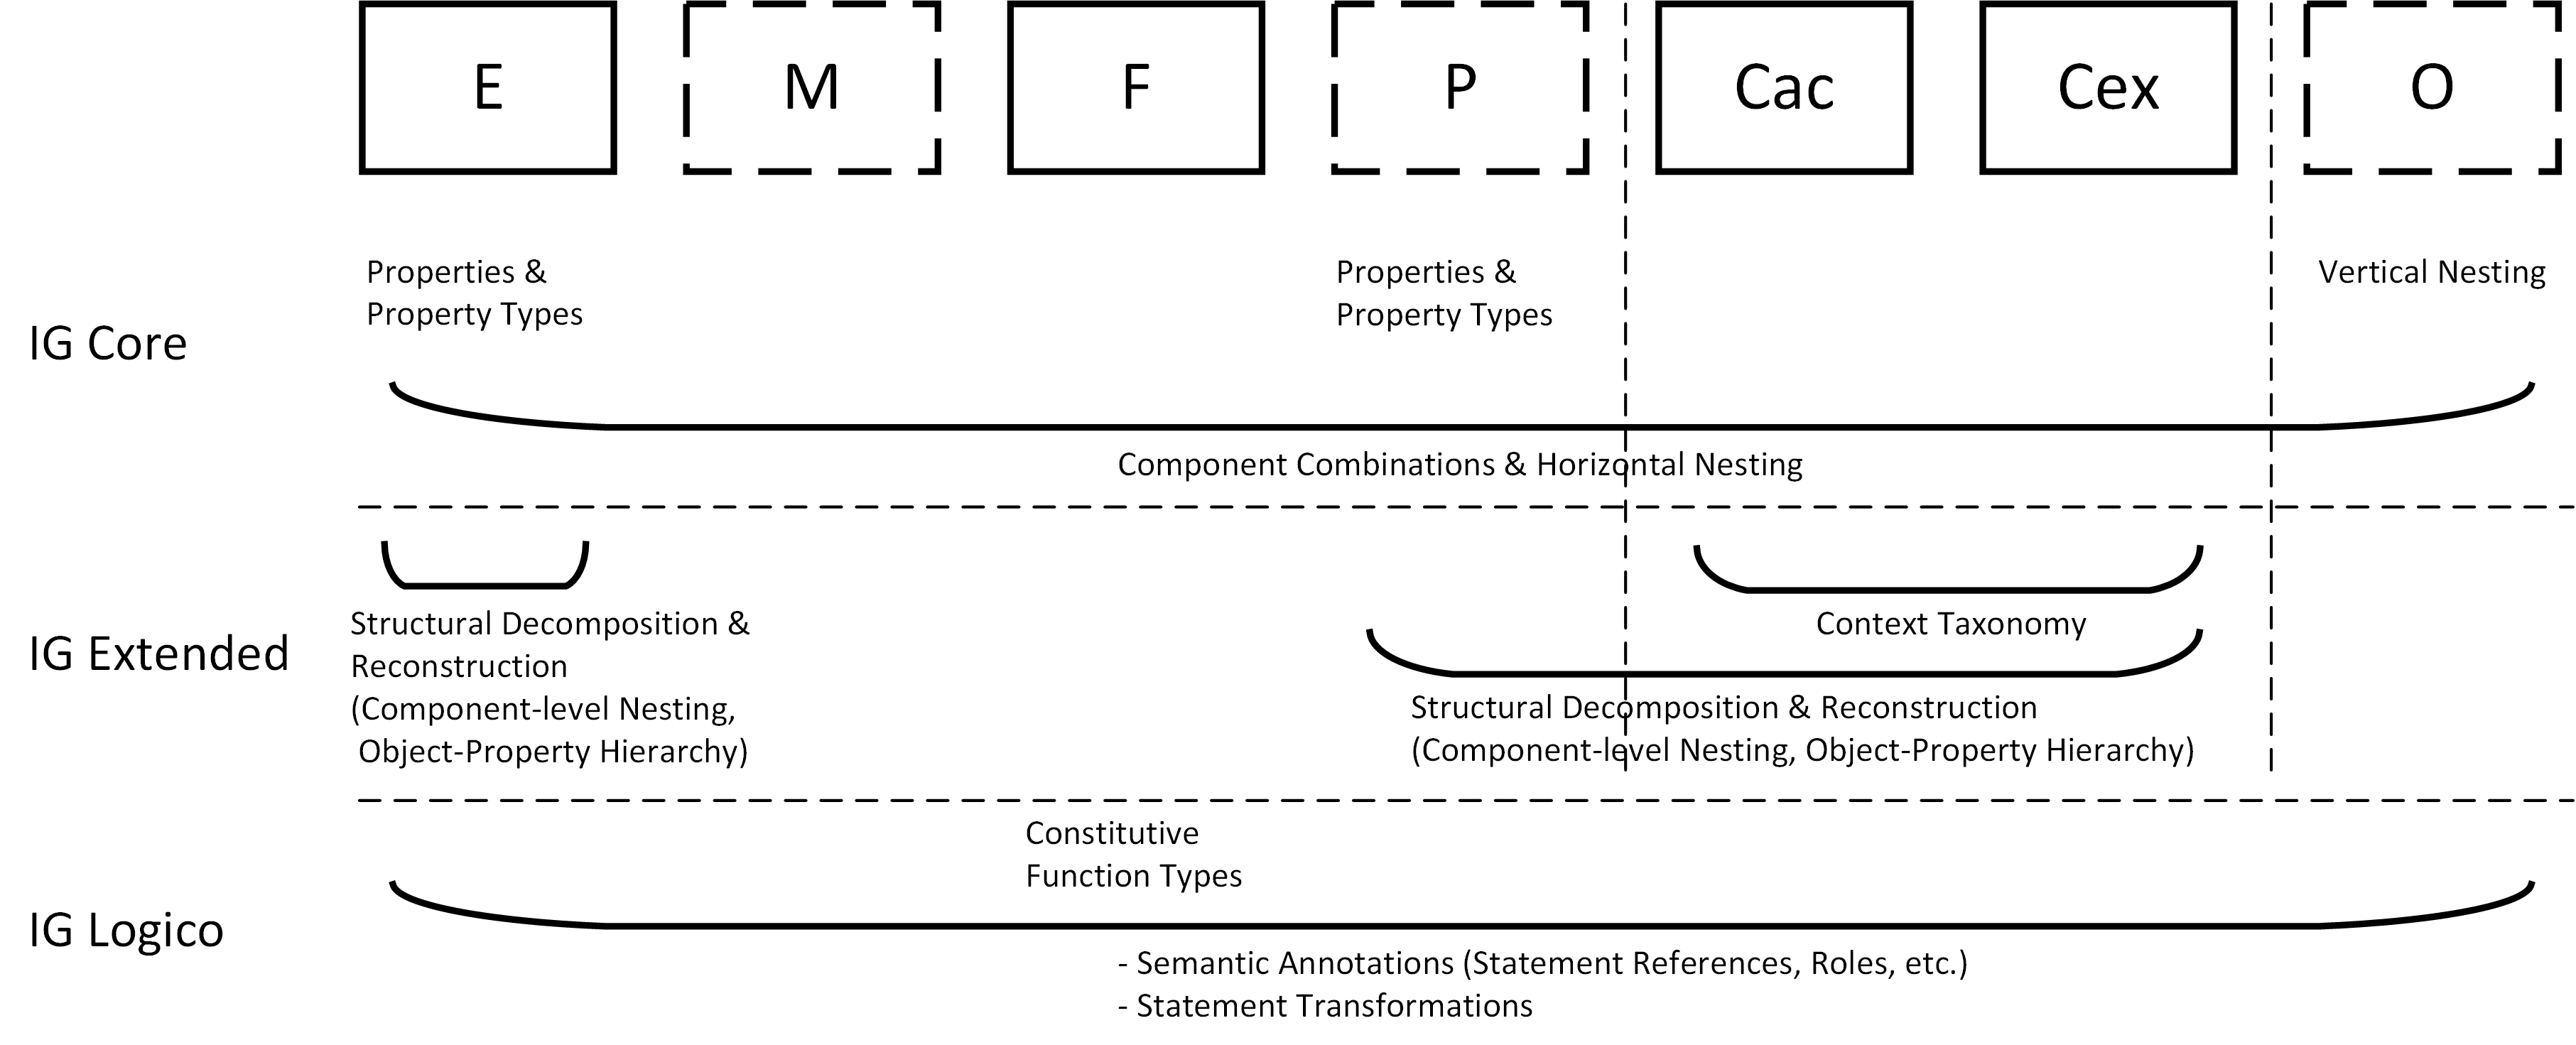
\includegraphics[width=0.95\textwidth]{figures/IGConstitutiveLevels.png}}
    \caption{Syntax and Features of Constitutive Statements by Level of Expressiveness}
    \label{fig:ConstitutiveStatementLevels}
\end{figure}

Motivating the principal coding of constitutive statements (without further elaboration at this stage), a stylized atomic constitutive statement, coded in shorthand form, thus reads: 

\begin{exa}
\Cacconst{}(In the context of organic farming),  \E{},\propconst{}(certified) \E{}(farmers) \F{}(are) \Pp{}(farmers)  \Pp{},\propconst{}(that have undergone a certification process) \Cexconst{}(following relevant procedural guidelines).
\end{exa}

\sp

Mirroring the introduction of coding guidelines for regulative statements, in \cref{tab:CodingIgCoreConstitutive} we provide the corresponding instructions for constitutive statements. Given the feature overlap between regulative and constitutive statements, we make reference to selected feature sets described in the context of regulative statements as part of the coding guidelines. As for regulative statements, symbols are color-coded to signal the association with features specific to IG Core, IG Extended or IG Logico. Symbols associated with IG Core features for constitutive statements are held in \textcolor{\corecolorconst}{\corecolorconstname}. As with regulative statements, symbols associated with IG Extended are held in \textcolor{\extendedcolor}{\extendedcolorname}, and features associated with IG Logico are displayed in \textcolor{\logicocolor}{\logicocolorname} color.

\begin{landscape}

\subsubsection{IG Core Coding of Constitutive Statements}
\label{subsubsec:IGCoreConstitutive}

\begin{longtable}{\tabledims}
\toprule
\multicolumn{4}{p{25cm}}{\textbf{Level of Expressiveness: IG Core}

\sp

IG Core enables basic, structural analysis of institutional statements. Encoding at this level is designed to be human readable and moderately comprehensive in the detail with which syntactic properties of institutional statements are captured.  
} \\

\newpage

\toprule

{\textbf{Syntactic\newline Component}} & 
{\textbf{Treatment of Syntactic Components by Level of Encoding}} &
{\textbf{Relevant Examples}} &
{\textbf{Complete Syntactic Classification of Examples}} \\
\toprule



\begin{emp}Constituted 

Entity\end{emp} 

&

The encoding of the Constituted Entity, which reflects any entity created, modified or otherwise introduced into the institutional setting. Constituted entities can be of physical or virtual nature, reflect concrete or abstract concepts, typically including actors, roles, actions, and objects. Constituted entities can further be differentiated into entity and entity property.

\sp

\udl{Note:} The separation of Constituted Entity and the associated properties operates identical to the decomposition of Attributes and Attributes properties. See corresponding guidelines provided under the Attributes component specification (see \hyperlink{tablink:AttributePropertyHeuristics}{here}).

&

\udl{Example statement:} 

\begin{exi}There is hereby established a public Food Security Advisory Board. \end{exi}

\sp

Entity = \begin{exi}Food Security Advisory Board\end{exi}

\sp

Entity property = \begin{exi}public\end{exi}

\sp


\udl{Example statement:}

\begin{exi}No member of the Council shall be disqualified from holding any public office or employment.\end{exi}

\sp

While reflecting structural patterns of regulative statements, this statement parameterizes members with respect to rights in the context of the Council.

\sp

Beyond the necessary components (\E, \F~and implied Context), the substantive characteristics that do \begin{emp}NOT\end{emp} apply (see negation applied) to the constituted entity are expressed as constituting properties.

\sp

\udl{Additional example:} 

\begin{exi}Established in this Regulation subpart is the right to appeal to a revocation or certification.\end{exi}

&

\vspace{0.05cm}

\begin{exi} There is \Cexconst{}(hereby) \F{}(established) a \E{},\propconst{}(public) \E{}(Food Security Advisory Board). \end{exi}




\vspace{2.45cm}

\begin{exi}\NOTconst{}(No) \E{}(member) of the \E{}, \propconst{}(Council) \M{}(shall) \F{}(be) \Pp{}(disqualified from holding any public office or employment).\end{exi}

\sp


 

\vspace{6.1cm}

\begin{exi}\F{}(Established) \Cexconst{}(in this Regulation subpart) is the \E{}(right to appeal) to a \E{},\propconst{}(revocation or certification).\end{exi}

\\ 

\begin{emp}Constituted Entity (ctd.)\end{emp}

&

&

Constitutive statements and Implied Attributes: In instances in which a coder is encountering ambiguity in discerning whether she is dealing with a constitutive or regulative statement, one shall consider the wider context of the statement (e.g., implied attribute, type of surrounding statements, etc.). A more detailed discussion can be found in \cref{subsec:SyntacticPolymorphs}.

& \\

\newpage

\midrule

\begin{exi}Constitutive Function\end{exi} &

The constitutive function characterizes the establishment, definition or introduction of a constituted entity into the institutional setting, and where constituting properties exist, functionally link constituted entity and constituting properties. 

&

\udl{Example statement:}

\begin{exi}There is hereby established a public Food Security Advisory Board.\end{exi}

\sp

Constitutive Function: \begin{exi}\lsi is\rsi~\dots~established\end{exi}

\sp

In this context the constitutive function signals the establishment of an entity.

\sp

\udl{Example:} 

\begin{exi}Commissioner of Agriculture and Markets shall be the Chairperson the Council.\end{exi}

\sp

Constitutive Function: \begin{exi}\lsi serve as\rsi\end{exi}

\sp

Here the constitutive function indicates a modified position (\begin{exi}Chairperson\end{exi}) of a specific role (\begin{exi}Commissioner\end{exi}) in a specific organizational context (\begin{exi}Council\end{exi}).

\sp

While diverse in nature, the constituting function can be sensibly organized along a set of patterns discussed in the context of IG Logico.

&

\vspace{0.03cm}

\begin{exi}There is \Cexconst{}(hereby) \F{}(established) a \E{},\propconst{}(public) \E{}(Food Security Advisory Board).\end{exi}

\vspace{3.5cm}

\begin{exi}\Pp{}(Commissioner of Agriculture and Markets) \M{}(shall) \F{}(be) the \E{}(Chairperson the Council).\end{exi}

\\

\newpage

\midrule

\begin{exi}Constituting Properties\end{exi}

&

Constituting properties are optional components in constitutive institutional statements that capture elements functionally linked to the constituted entity by means of the constitutive function. 

Constituting properties may themselves have properties.

\sp

\udl{Note:} The separation of Constituting Properties and the associated nested properties operates identical to the decomposition of Attributes and Attributes properties. See corresponding guidelines provided under the Attributes component specification (see \hyperlink{tablink:AttributePropertyHeuristics}{here}).

&

\udl{Example:} 

\begin{exi}The Committee shall consist of a President, Secretary, and Treasurer.\end{exi}

\sp

Constituting properties: \begin{exi}President, Secretary, and Treasurer\end{exi}

\sp

Here, the council is composed of the members as constituting properties.

\sp

\udl{Example:} 

\begin{exi}A majority of the members of the Council shall constitute a quorum.\end{exi}

\sp

Constituting properties: \begin{exi}majority of the members of the Council\end{exi}

&

\vspace{0.03cm}

\begin{exi}The \E{}(Committee) \M{}(shall) \F{}(consist) of a \Pp{}(President, Secretary, and Treasurer).\end{exi}

\vspace{3.55cm}

\begin{exi}A \Pp{}(majority of the members of the Council) \M{}(shall)
\F{}(constitute) a \E{}(quorum).\end{exi}


\\

\midrule

\begin{emp}Modal\end{emp} &

The Modal signals the extent to which the instruction contained in the constitutive statement is required (necessary), or signals mere possibility, (effectively mirroring the prescriptive and discretionary notion on the regulative side). Linguistically, the expression can be ambiguous between the regulative and constitutive variant (e.g., must, may, must not), but the coder should make an attempt to classify the modal from an epistemic perspective (i.e., focusing on necessity and possibility of the activity expressed in the constitutive function). Note that in constitutive statements the use of the modal can follow legal traditions or be stylistic in kind. The coder should acquaint oneself with such specifics prior to the coding.

&

\udl{Example:} 

\begin{exi}A majority of the members of the Council shall constitute a quorum.\end{exi}

\sp

Modal: \begin{exi}shall\end{exi}

\sp

Here \begin{emp}shall\end{emp} signals the necessity that a quorum means ``majority of the members of the Council'' in the context of the policy. 

\sp

\udl{Example:}

\begin{exi}The Council may have an advisory committee.\end{exi}

\sp

Modal: \begin{exi}may\end{exi}

\sp

Here \begin{emp}may\end{emp} signals the possibility (but not requirement) that the Council has an advisory committee. 

&

\vspace{0.02cm}

\begin{exi}
A \Pp{}(majority of the members of the Council) \M{}(shall) \F{}(constitute) a \E{}(quorum).\end{exi}

\vspace{4.0cm}

\begin{exi}
The \E{}(Council) \M{}(may) \F{}(have) an \Pp{}(advisory committee).\end{exi}

\\

\newpage

\midrule

\begin{emp}Context\end{emp} &

The encoding identifies the Context of the institutional statement. The encoding differentiates between ``Activation Conditions,'' which are contextual clauses that specify preconditions under which the statement applies, and ``Execution Constraints,'' which are contextual descriptors that qualify the constituting function by augmenting the statement with temporal, spatial, procedural, and/or other constraining parameters. &

\udl{Example statement:} 

\begin{exi}From 1st of January onward, food preparation guidelines must adhere to national standards, in addition to communal provisions.\end{exi}

\sp

Context clauses: \begin{exi}From 1st of January onward; in addition to communal provisions\end{exi}

\sp

\udl{Context encoding:} 

\sp

Activation Condition: \begin{exi}From 1st of January onwards\end{exi}

\sp

Execution Constraint: \begin{exi}in addition to communal provisions\end{exi}

\sp

The activation condition signals an event that initiates a discretized setting in which the remaining statement holds.

\sp

The execution constraint characterizes the constitutive function more explicitly. 

&

\begin{exi}\udl{\Cacconst{}(From 1st of January onward)}, \E{}(food preparation guidelines) \M{}(must) \F{}(adhere) to \Pp{}(national standards), \udl{\Cexconst{}(in addition to communal provisions)}.\end{exi}


\\

%\newpage

\midrule

\begin{emp}Or else\end{emp} &

The encoding of Or else statements identifies consequences of non-fulfillment or violation of institutional statements, which, in the context of constitutive statements, can signal consequences addressing specific actors (e.g., consequences in regulative terms), or be of existential nature. Existential nature signals that an establishment or modification of an entity may simply not come about, or that alternative or linked constitutive statements are instantiated. The encoding captures these consequences generally in the form of institutional statements that nest on the leading monitored institutional statement, and can be expressed both in regulative or constitutive form (see \cref{subsec:ConstitutiveRegulativeHybrids} for conceptual details on mixed statement types).

Principles of horizontal and vertical nesting (see \cref{subsec:InstitutionalStatementAssumptions}), as described in the regulative context (see \cref{subsec:RegulativeStatementCoding}), equally apply for constitutive statements, and within or else components.

Vertical nesting is applicable when there is at least one activity that is specified within a distinct institutional statement and activated as a consequence of a non-fulfilled action specified in the leading institutional statement. Horizontal nesting is applicable when there exist two or more activities that can be enacted in some logical combination as shown below. 

&

\udl{Example:} 

\begin{exi}
In student recruitment plans, diversity must mean diversity in race, religion, sexual orientation and gender, or else plan is void.
\end{exi}

\sp

Or else clause comprising statement: \begin{exi}or else plan is void\end{exi}

\sp

The Or else signals an existential consequence for the constituted entity as expressed by the necessity that diversity is defined as prescribed (\begin{emp}``must mean''\end{emp}).

\sp

Naturally, the consequence can also consist of multiple statements that are logically combined (horizontal nesting), as shown below.

\sp

\udl{Example:}


\begin{exi}
In student recruitment plans, diversity must mean diversity in race, religion, sexual orientation and gender, or else plan is void and to be revised within 30 days.\end{exi}


&

\vspace{0.05cm}

\begin{exi}
\Cacconst{}(In student recruitment plans), \E{}(diversity) \M{}(must) \F{}(mean) \Pp{}(diversity in race, religion, sexual orientation and gender), 

or else

\Oeconst{}\lb \E{}(plan) \F{}(is) \Pp{}(void)\rb .\end{exi}

\vspace{6.5cm}

\begin{exi}
\Cacconst{}(In student recruitment plans), \E{}(diversity) \M{}(must)  \F{}(mean) \Pp{}(diversity in race, religion, sexual orientation and gender), 

or else 

\Oeconst{}\lb \lb \E{}(plan) \F{}(is) \Pp{}(void)\rb

\ANDconst

\lb \dots~\E{}(plan) \F{}(is~\dots~to be revised) \Cexconst(within 30 days)\rb \rb .\end{exi}

\sp

In the previous example, horizontal nesting is signaled using braces around statements (as opposed to individual components), and vertical nesting is likewise expressed using braces (\lb~and \rb ) scoped around the compound consequence. 

\\

\begin{emp}Or else (ctd.)\end{emp}

&

These statement combinations can signal 

\begin{itemize}
\item alternative exclusive action options -- \XORconst s -- (e.g., either initiate XOR expand the Council),
\item inclusive action options -- \ORconst s -- (e.g., rights may be assigned AND/OR responsibilities removed when an individual is added to the Council) or 
\item co occurring action options -- \ANDconst s -- (e.g., dissolving a Council AND compensating Council members)
\end{itemize}

&

\udl{Note:}

\begin{enumerate}
\item Where component combinations exist, alternatives are combined (\dots~are void and to be refined fine farmer or revoke \dots), and are subsequently decomposed into separate logically-combined complete atomic institutional statements. 
\item Ambiguities with respect to the linguistic use of logical operators (exclusive and inclusive or) are to be resolved as part of this process. 
\end{enumerate}

&

\\

\midrule

\newpage

%\toprule
%\multicolumn{4}{p{17cm}}{\textbf{General IG Core instructions (equivalent to regulative statements)}}

%\toprule

\midrule
\multicolumn{4}{l}{\textbf{General IG Core Instructions for Constitutive Statements}} \\
\midrule


\begin{emp}Additional annotations for Constituted Entity, Constitutive Function, Constituting Property and Context\end{emp}

\sp

(\udl{Note:} This feature is analogous to the specification of additional annotations for Attribute, Object and Context components in the context of regulative statements.) 

&

In addition to the identification of properties embedded in the original statements, components can further be annotated using additional annotation labels. Such labels can follow the categories listed in \cref{sec:Taxonomies}, or be specific to the project objectives.

\sp

A systematic approach to labelling entities is discussed under \hyperlink{tablink:CrossComponentSemanticAnnotationsLogicoRegulative}{\begin{emp}IG Logico Instructions\end{emp}, Item \EntryCrossComponentSemanticAnnotations} in \cref{tab:CodingIgLogicoRegulative}. This is particularly recommended if annotations are of strong relevance for the coding and of diverse nature. 

&

\udl{Example:} 

\begin{exi}The Committee shall consist of a President, Secretary, and Treasurer.\end{exi}

\sp

Subject to analytical necessity, additional annotations can for instance relate to the identification of aspects, such as the characterisation of encoded objects with respect to their animacy as either animate or inanimate -- signified in brackets in the coded example. Where indicated, the annotation should be separated from the component specification by semicolon and have the structure ``label='', followed by the annotation. 

Note that ``\begin{exi}label\end{exi}'' is a characterizing prefix, either based on a specific taxonomy (see \cref{sec:Taxonomies} for an overview), or a custom coder-defined category specification (e.g., defined as part of the project-specific guidelines). In this example, the Animacy Taxonomy has the prefix ``\anim'' as defined in \cref{sec:Taxonomies} and is used correspondingly.

\sp

While exemplified here for constitutive statements, this equally applies to regulative statements. 

&

\vspace{0.03cm}

\begin{exi}The \E{}\customLog{\anim=inanimate}(Committee) \M{}(shall)  \F{}(consist of) a \Pp{}\customLog{\anim=animate}(President, Secretary, and Treasurer).\end{exi}

\\

\midrule

\hypertarget{tablink:DecompositionOfComponentLevelCombinationsCoreConstitutive}{\EntryDecompositionOfComponentLevelCombinations}

\sp

(Note: This applies to regulative and constitutive statements, and is discussed here with focus on the constitutive perspective.)

&

Where combinations of components (component-level combinations) are observed that are not explicitly decomposed as in the case of vertical nesting, these can be decomposed into logically-combined statements. 
Other than for constitutive functions, the decomposition is optional for IG Core. 

Operationally, combinations of components are evidenced by the presence of multiple logically-combined tokens or clauses embedded in constituted entities, constitutive functions, constituting properties or context components. 

Decomposition essentially entails constructing an individual statement to capture each of the unique components represented in multiples within institutional statements, noting the relation to the original statement in which multiple components are reflected. Information from component fields, other than that containing multiple components, is simply carried over to all related institutional statements. 

Importantly, where decomposition actually changes the meaning of the original institutional statement containing multiple components within a particular syntactic field, the statement should not be decomposed. In such cases, multiples are typically intended to exist in coupled form. An example is provided in the next column.


&

Details are described in the 
\hyperlink{tablink:DecompositionOfComponentLevelCombinationsExtendedRegulative}{\begin{emp}General IG Extended Instructions\end{emp}, Item \EntryDecompositionOfComponentLevelCombinations} in \cref{tab:CodingIgExtendedRegulative}.

\sp

\udl{Example (Multiple Properties):} 

\begin{exi}The Committee shall consist of a President, Secretary, and Treasurer.\end{exi}

\sp

While expressed in condensed form as ``\begin{exi}The \E{}(Committee)  \M{}(shall) \F{}(consist of) a \Pp{}(\lpconst President \AND{}~Secretary \AND{}~Treasurer\rpconst)\end{exi}'' (note the parentheses),

\sp

it corresponds to the following statement composed of three atomic statements:

\sp

\udl{Statement 1:} \begin{exi}The Committee shall consist of a President\end{exi}

\sp

\ANDconst

\sp

\udl{Statement 2:} \begin{exi}The Committee shall consist of a Secretary.\end{exi}

\sp

\ANDconst 

\sp

\udl{Statement 3:} \begin{exi}The Committee shall consist of a Treasurer.\end{exi}

\sp

\udl{Example (Multiple constitutive functions):} \begin{exi}The form and function of the Council is hereby established.\end{exi}

\sp

&

\udl{Condensed form:}

\begin{exi}The \E{}(Committee) \M{}(shall) \F{}(consist of) a \Pp{}(\lpconst President \ANDconst~Secretary
\ANDconst~Treasurer\rpconst).\end{exi}

\sp

\udl{Expanded form:}

\begin{exi}\lb \lb The \E{}(Committee) \M{}(shall) \F{}(consist of) a \Pp{}(President)\rb

%\sp

\ANDconst

%\sp

\lb The \E{}(Committee) \M{}(shall) \F{}(consist of) a \Pp{}(Secretary)\rb

%\sp

\ANDconst 

%\sp

\lb The \E{}(Committee) \M{}(shall) \F{}(consist of) a \Pp{}(Treasurer)\rb \rb .\end{exi}



\vspace{8.6cm}




\begin{exi}
\lb \lb \E{}(Council form) is \Cexconst{}(hereby) \F{}(established)\rb

%\sp

\ANDconst

%\sp

\lb \E{}(Council function) is \Cexconst{}(hereby) \F{}(established).\rb \rb
\end{exi}

\\

\begin{emp}Decomposition of component-level combinations (ctd.)\end{emp}

&

&

\udl{Note:} These guidelines highlight the motivation for the decomposition, and exemplify it explicitly. Depending on the use of annotation means and tool support, the decomposition may be partially automated, affording a mere annotation for such decomposition without requiring the user to perform statement duplication.

&

\\

\toprule
\caption{Coding Guidance on Syntactic Elements for IG Core as Level of Expressiveness (Constitutive Statements)}
\label{tab:CodingIgCoreConstitutive}
\end{longtable}

\newpage

\subsubsection{IG Extended Coding of Constitutive Statements}
\label{subsubsec:IGExtendedConstitutive}

\begin{longtable}{\tabledims}

\toprule
\multicolumn{4}{\tablespan}{\textbf{Level of Expressiveness: IG Extended}

\sp

Mirroring the progression on the regulative side, IG Extended enables more detailed structural analysis of institutional data than IG Core and accommodates computational application to aid in institutional coding and analysis. Encoding at this level is designed to be human readable, moderately computationally tractable, and moderately comprehensive in the detail with which syntactic properties of institutional statements are captured. 

\sp 

Coding institutional statements on this level enforces many of the features that have been optional in IG Core and affords a fine-grained decomposition of statements. This includes a richer context characterization based on predefined taxonomies, the expansion and combined attributes and aims that reconstruct atomic statements and their relationships, but also decomposes the hierarchical relationships amongst explicitly highlighted Constituted Entities, Constituting Properties and Constitutive Functions, alongside further refinements of contextual descriptors.

\sp

As a central feature IG Extended makes the use of component-level combinations explicit. This specifically facilitates the decomposition of the context component to express institutional content at a more nuanced level. In addition, structural refinements relate to the decomposition of relationships and properties of Constituted Entities and Constituting Properties.

\sp

For constitutive statements, IG Extended features correspond to the regulative side, with the essential difference for the application of refinements on Attributes and Objects, which, in the context of constitutive statements apply to Constituted Entities and Constituting Properties. 

\sp

A specific consideration is the concept of Constitutive-Regulative Hybrids and syntactic polymorphs, both of which are of cross-cutting nature (i.e., affecting both constitutive and regulative statements) and thus discussed in a dedicated section. Their consideration, however, applies to IG Extended.

} \\
\toprule

{\textbf{Syntactic\newline Component}} & 
{\textbf{Treatment of Syntactic Components by Level of Encoding}} & 
{\textbf{Relevant Examples}} &
{\textbf{Complete Syntactic Classification of Examples}} 
\\

\toprule

\begin{emp}
Constituted 

Entity
\end{emp}

&

In IG Extended encoding, Constituted Entities and their properties are decomposed hierarchically following the principles of the Object-Property Hierarchy (\cref{subsec:AttributeObjectHierarchy}) and is applied analogous to ``Attributes'' in IG Extended for regulative statements (\cref{tab:CodingIgExtendedRegulative}). The ensuing overview of constituted properties shows an extended set of examples applied analogously to constituted entities.

&

\udl{Example:}\newline
\begin{exi}There is hereby established a standing public Food Security Advisory Board.\end{exi}

& 

\begin{exi}There is \Cexconst \customExt{ctx=met}(hereby) \F{}(established) a \E{},\propExt{1}(standing) \E{},\propExt{2}(public) \E{}(Food Security Advisory Board).\end{exi} 

\\

\midrule

\begin{emp}
Constituting 

Property
\end{emp}

&

%\multicolumn{3}{\tablespanNarrow}{

Analogous to the decomposition of object properties in the context of regulative statements, constituting properties are likewise decomposed following the principles of the Object-Property Hierarchy (as introduced in \cref{subsec:AttributeObjectHierarchy} and applied in the context of ``Objects'' in IG Extended for regulative statements in \cref{tab:CodingIgExtendedRegulative}). 

%} 

&

\udl{Example:}\newline
\begin{exi}The Council consists of  elected officials resident in the electorate.\end{exi}

\sp

In this example, the individual properties of the constituting property \begin{emp}officials\end{emp}, namely \begin{emp}elected\end{emp} and \begin{emp}resident in the electorate\end{emp}, are uniquely identified as properties.

\sp

Another feature is the richer hierarchical structure embedded in phrase expressing compound property characterizations. 

\sp

\udl{Example:}\newline
\begin{exi}A majority of the members of the Council shall 
constitute a quorum.\end{exi}

\sp

In this example, the constituting property is captured in the phrase  \begin{emp}A majority of the members of the Council\end{emp}. While the entire phrase represents the constituting property (and is coded as such on IG Core), the embedded hierarchy, i.e., members are a property of the Council, and the majority is a property of the members, can be explicitly captured using hierarchical property annotations as shown on the right. 

Where properties are not functionally dependent on another property, they are signaled using unique identifiers (e.g., \PpExt{a}, \PpExt{b}) equivalent to ``Object'' decomposition highlighted in \cref{tab:CodingIgExtendedRegulative} and exemplified in the following.

&

\vspace{0.02cm}

\begin{exi}The \E{}(Council) \F{}(consists of) \Pp{},\propExt{1}(elected) \Pp{}(officials) \Pp{},\propExt{2}(resident in the electorate).\end{exi}

\vspace{5.6cm}

\begin{exi}A \Pp{},\propExt{1},\propExt{1}(majority) of the \Pp{},\propExt{1}(members) of the \Pp{}(Council) \M{}(shall) \F{}(constitute) a \E{}(quorum).\end{exi}

\\

\begin{emp}
Constituting 

Property (ctd.)
\end{emp}

&

&

Collections of functionally independent entities are represented as a compound constituting property signaled by parentheses. Individual compound properties can be uniquely identified, alongside potential further properties shared across all embedded entities.\footnote{Specific data structure patterns commonly found in institutional statements are revisited in \cref{subsec:DataStructurePatterns}.}

\sp

\udl{Example:}\newline
\begin{exi}The Committee shall consist of a President, Secretary, and qualified Treasurer appointed by the public.\end{exi}

\sp

In this example, properties specific to an entity are called out with reference to the entity (\begin{emp}qualified\end{emp}), whereas shared properties are associated with all entities (\begin{emp}appointed by the public\end{emp}).

& 

\vspace{4.1cm}

\begin{exi}The \E{}(Committee) \M{}(shall) \F{}(consist of) a \Pp{}(\lpconst  \PpExt{1}(President) \ANDconst~\PpExt{2}(Secretary)
\ANDconst~\PpExt{3},\propExt{1}(qualified) \PpExt{3}(Treasurer)\rpconst )~\Pp,\propconst{}(appointed by the public).\end{exi}

\\

\midrule

\begin{emp}
Context
\end{emp}

&

\multicolumn{3}{\tablespanNarrow}{
See ``Context'' in IG Extended for regulative statements (\cref{tab:CodingIgExtendedRegulative})

} \\

\midrule
\begin{emp}
General IG 

Extended Instructions
\end{emp}
&

\multicolumn{3}{\tablespanNarrow}{
See ``General IG Extended Instructions'' in IG Extended for regulative statements (\cref{tab:CodingIgExtendedRegulative})
} \\

\midrule

\begin{emp}
Constitutive-

regulative Hybrids
\end{emp}

&

\multicolumn{3}{\tablespanNarrow}{
The introduction of constitutive statements as part of IG 2.0 (see \cref{subsec:ConstitutiveStatementCoding}) provides the basis for encoding statements that consist of structural elements both of regulative and constitutive statements. Details are discussed in \cref{subsec:ConstitutiveRegulativeHybrids}.

} \\

\toprule

\caption{Coding Guidance on Syntactic Elements for IG Extended as Level of Expressiveness (Constitutive Statements)}
\label{tab:CodingIgExtendedConstitutive}
\end{longtable}

\newpage

\subsubsection{IG Logico Coding of Constitutive Statements}
\label{subsubsec:IGLogicoConstitutive}

\begin{longtable}{\tabledims}
\toprule
\multicolumn{4}{\tablespan}{\textbf{Level of Expressiveness: IG Logico}

\sp

IG Logico is designed to support semantic analysis of institutional statements wholly relying on computational tools. Encoding at this level is designed to be moderately human readable, computationally tractable and comprehensive in the detail with which syntactic properties of institutional statements are captured. 

\sp

In contrast to IG Core and Extended that focus on the encoding of specific grammar components, IG Logico emphasises refinements across individual components and further establishes explicit references to related statements to establish computational tractability, as well as the ability to perform logical transformations on institutional statements. 

\sp

While largely equivalent for regulative and constitutive statements, the only variant to the instructions provided in the context of regulative statements is the discussion of Constitutive Function taxonomies (as opposed to Institutional Functions in the context of regulative statements) as outlined below.

}\\

\newpage

\toprule

{\textbf{Syntactic\newline Component}} & 
{\textbf{Treatment of Syntactic Components by Level of Encoding}} &
{\textbf{Relevant Examples}} &
{\textbf{Complete Syntactic Classification of Examples}} \\

\toprule

\begin{emp}Constitutive Function Annotations\end{emp} 

&

Complementing the content characterization for other components, the constitutive function maintains the central role as a descriptor of constituted entities, and where constituting properties exist, links those to constituted entities. 

\sp

In an attempt to characterize the function of the constitutive statement as expressed in the constitutive function more generally, we propose a taxonomy capturing common relationships more generally. Doing so, we differentiate between statements that characterize the constituted entity as newly introduced into the institutional setting, and a commonly found alternative, that is, the characterization of the policy that contains the statements itself.

\sp

Entities, such as novel actors, objects, roles or action, can be 
\begin{itemize}
\item defined explicitly (``is'', ``does''), 
\item defined based on relationships, such as composition (``consists of''), organizational embedding (``is embedded in'', ``relates to''), 
\end{itemize}

&

\udl{Example:} 

\begin{exi}
Starting January 1st, the Connecticut Food Policy Council shall be within the Department of Agriculture.
\end{exi}

\sp

In this example the constitutive function signals the constituted entity (Connecticut Food Policy Council) as an organizational unit.

\sp

\udl{Example:} 

\begin{exi}
The Committee shall consist of a President, Secretary, and Treasurer.
\end{exi}

\sp

The constitutive function signals a composition of the constituted entity (\begin{exi}Committee\end{exi}) based on constituting properties. 

\sp

\udl{Example:} 

\begin{exi}The purpose of this Part is to establish standards for net metering in accordance with the requirements of Section 16-107.5 of the Act.\end{exi}

\sp

In this example, the constitutive function identifies the entity as a policy and signals the intent underlying the policy. 

&

\vspace{0.03cm}

\begin{exi}
\Cacconst{}(Starting January 1st), the \E{}(Connecticut Food Policy Council) \M{}(shall) \F{}\customLog{\confunc=organization}(be within) the \Cexconst{}(Department of Agriculture).\end{exi}

\vspace{2.5cm}

\begin{exi}
The \E{}(Committee) \M{}(shall) \F{}\customLog{\confunc=composition}(consist of) a \Pp{}(\lpconst President \ANDconst~Secretary
\ANDconst~Treasurer\rpconst).\end{exi}

\vspace{1.55cm}

\begin{exi}
The \E{}(purpose of this Part) \F{}\customLog{\confunc=intent}(is) \Pp{}(to establish standards for net metering in accordance with the requirements of \customLog{\polref=Section/16-107.5}(Section 16-107.5) of the Act).\end{exi}

\\

\begin{emp}Constitutive Function Annotations (ctd.)\end{emp}

&

\begin{itemize}
\item defined based on lifecycle stages (``established'', ``terminated''), and finally 
\item characterized by the conferral of status in the form of rights, authority, or exertion of institutional power more generally.
\end{itemize}

Policies as constituted entities in institutional statements, in contrast, are generally referred to with respect to the 
\begin{itemize}
\item lifecycle stage they are involved in (``come into force''), 
\item relationship between and to other statements or policies (``amends'', ``substitutes''), 
\item intent in the form of purpose of a specific policy, and appear as 
\item information statements that offer information about the policy itself.
\end{itemize}

%\sp

Naturally, these characterizations are not exhaustive and can carry more specific forms. An overview of the different characterizations, alongside the labels used in this context is provided in \cref{sec:Taxonomies}.

& 

\udl{Example:}

\begin{exi}In department's university plan, diverse population means diversity in religion, sexual orientation and race.\end{exi}

\sp

In this example, the constituted entity is defined intensionally, that is in terms of its underlying interpretations.

& 

\vspace{0.03cm}

\begin{exi}
\Cacconst{}\customExt{ctx=dom}(In department's university plan), \E{}(diverse population) \F{}\customLog{\confunc=definition}(means) \Pp{}(\lp diversity in religion \AND{}~sexual orientation \AND{}~race\rp).\end{exi}

\\

\toprule

\caption{Coding Guidance on Syntactic Elements for IG Logico as Level of Expressiveness (Constitutive Statements)}
\label{tab:CodingIgLogicoConstitutive}
\end{longtable}

\end{landscape}

\subsection{Hybrid \& Polymorphic Institutional Statements}
\label{subsec:ConstitutiveRegulativeHybrids}

In addition to the specific treatment of regulative and constitutive statements as part of the coding guidelines, an aspect that demands specific attention is the combined use of both statement types. While distinctively different in their function, regulative and constitutive statements, of course, share structural patterns as outlined in the context of the operational coding across varying levels of expressiveness.

\sp

However, an operational concern that links both statement types is the interleaved use in practice. In addition to the commonly found organization of primarily constitutive and regulative statements into distinctive sections of documents (e.g., constitutive statements as part of the preamble), in regulative statements we may encounter inline specifications of entities that are positioned in the institutional setting and are thus of relevance for subsequent statements. Conversely, in constitutive statements, we can potentially encounter embedded regulative elements that regulate behavior of the constituted entities. Linking the nested relationships of institutional statements across both types, we recognize the concept of \begin{emp}hybrid institutional statements\end{emp}, in which the combined use of constitutive and regulative statements can either take constitutive-regulative form (where the overall statement is of constitutive nature) or be a regulative-constitutive hybrid (where the leading statement is of regulative nature). 
Where existing, their resolution is a central feature of IG Extended onwards (and optional for IG Core). 

In contrast to statements that embed a combination of parameterizing and regulating features, in specific instances statements may be encodeable in both regulative and constitutive form. While such variable coding often reflects a concession to analytical objectives, potential coding inconsistencies can be resolved by a priori specification of the interpretational scope applied in the coding process (see \cref{subsec:StatementTypesHeuristics}). Where a generic coding of statements, agnostic of analytical uses, is desired, statements can be coded as \begin{emp}polymorphic institutional statements\end{emp} that allow the concurrent encoding in different statement forms. This special form of institutional statements is discussed in \cref{subsec:SyntacticPolymorphs}.

Initially, however, we will exemplify both variants of statement hybrids.

\subsubsection{Regulative-Constitutive Statements}

A typical reflection of hybrids stems from the introduction of novel entities as part of a regulative statement, as shown in the following example (\cref{fig:RegulativeConstitutiveHybridRaw}):

\begin{figure}[h!]
    \centering
    \framedfigure{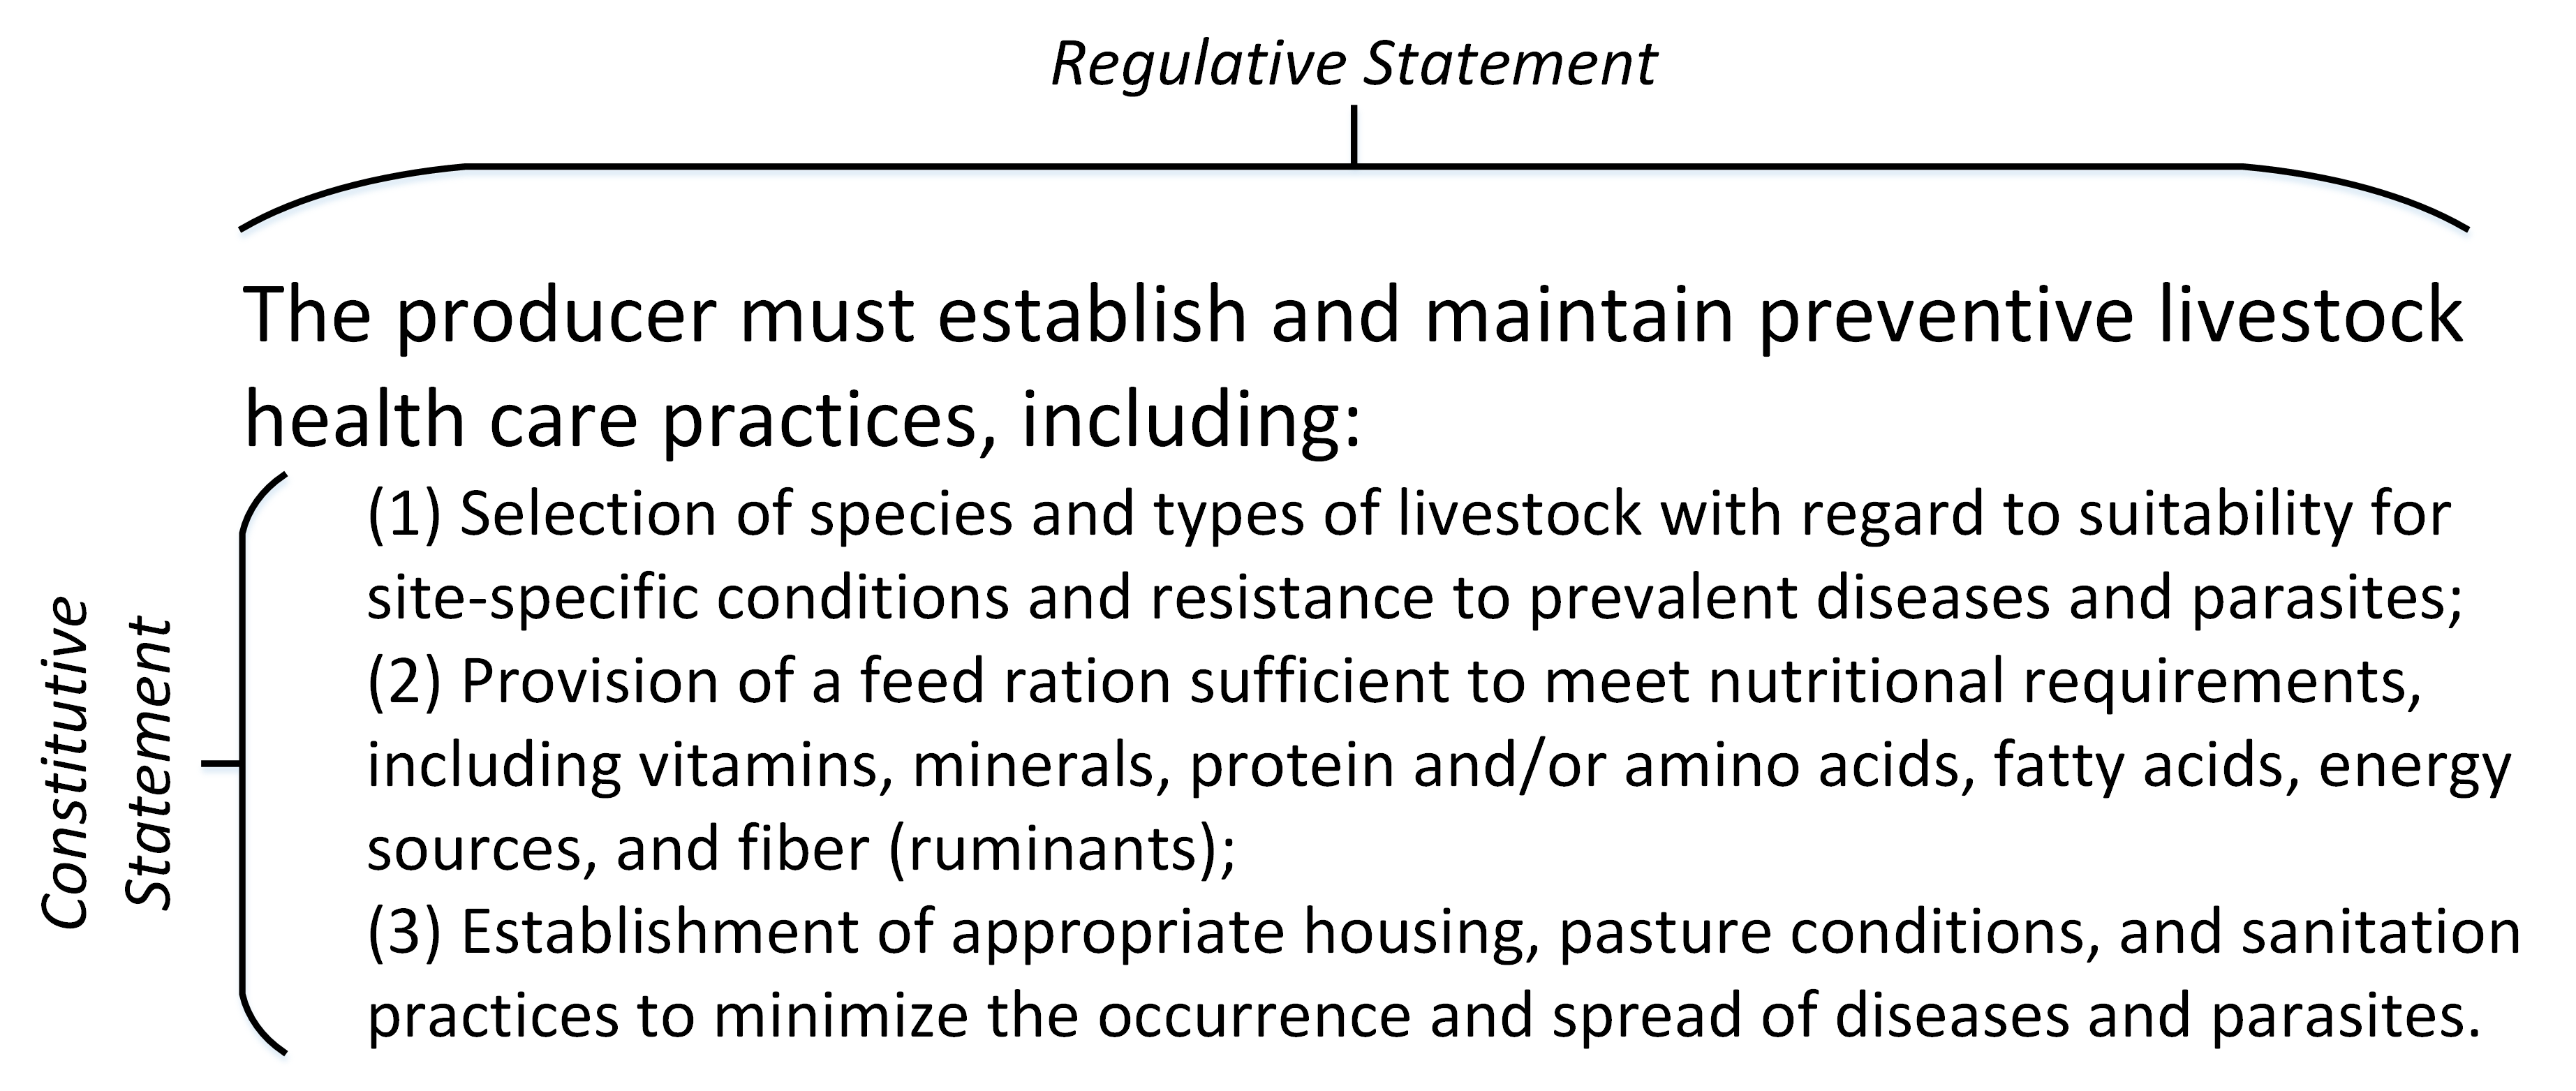
\includegraphics[width=0.8\textwidth]{figures/RegulativeConstitutiveHybridRaw.png}}
    \caption{Regulative-Constitutive Hybrid Example}
    \label{fig:RegulativeConstitutiveHybridRaw}
\end{figure}

As signaled visually, this example highlights a regulative statement capturing an actor's obligations, with the latter defined in an embedded constitutive statement, reflecting a regulative-constitutive hybrid. In this example, the constitutive statement is nested in a specific component of the regulative statement, such as the object as shown in the example in \cref{fig:RegulativeConstitutiveHybridCoded}. Note that the following figures use the same color-coding used in the preceding sections: Symbols associated with IG Core features for regulative statements are displayed in \textcolor{\corecolor}{\corecolorname}, whereas symbols signaling constitutive statements are held in \textcolor{\corecolorconst}{\corecolorconstname}.\footnote{In the context of this section, parentheses and logical operators are color-coded to emphasize the association with the corresponding institutional statement type.} 

\begin{figure}[h!]
    \centering
    \framedfigure{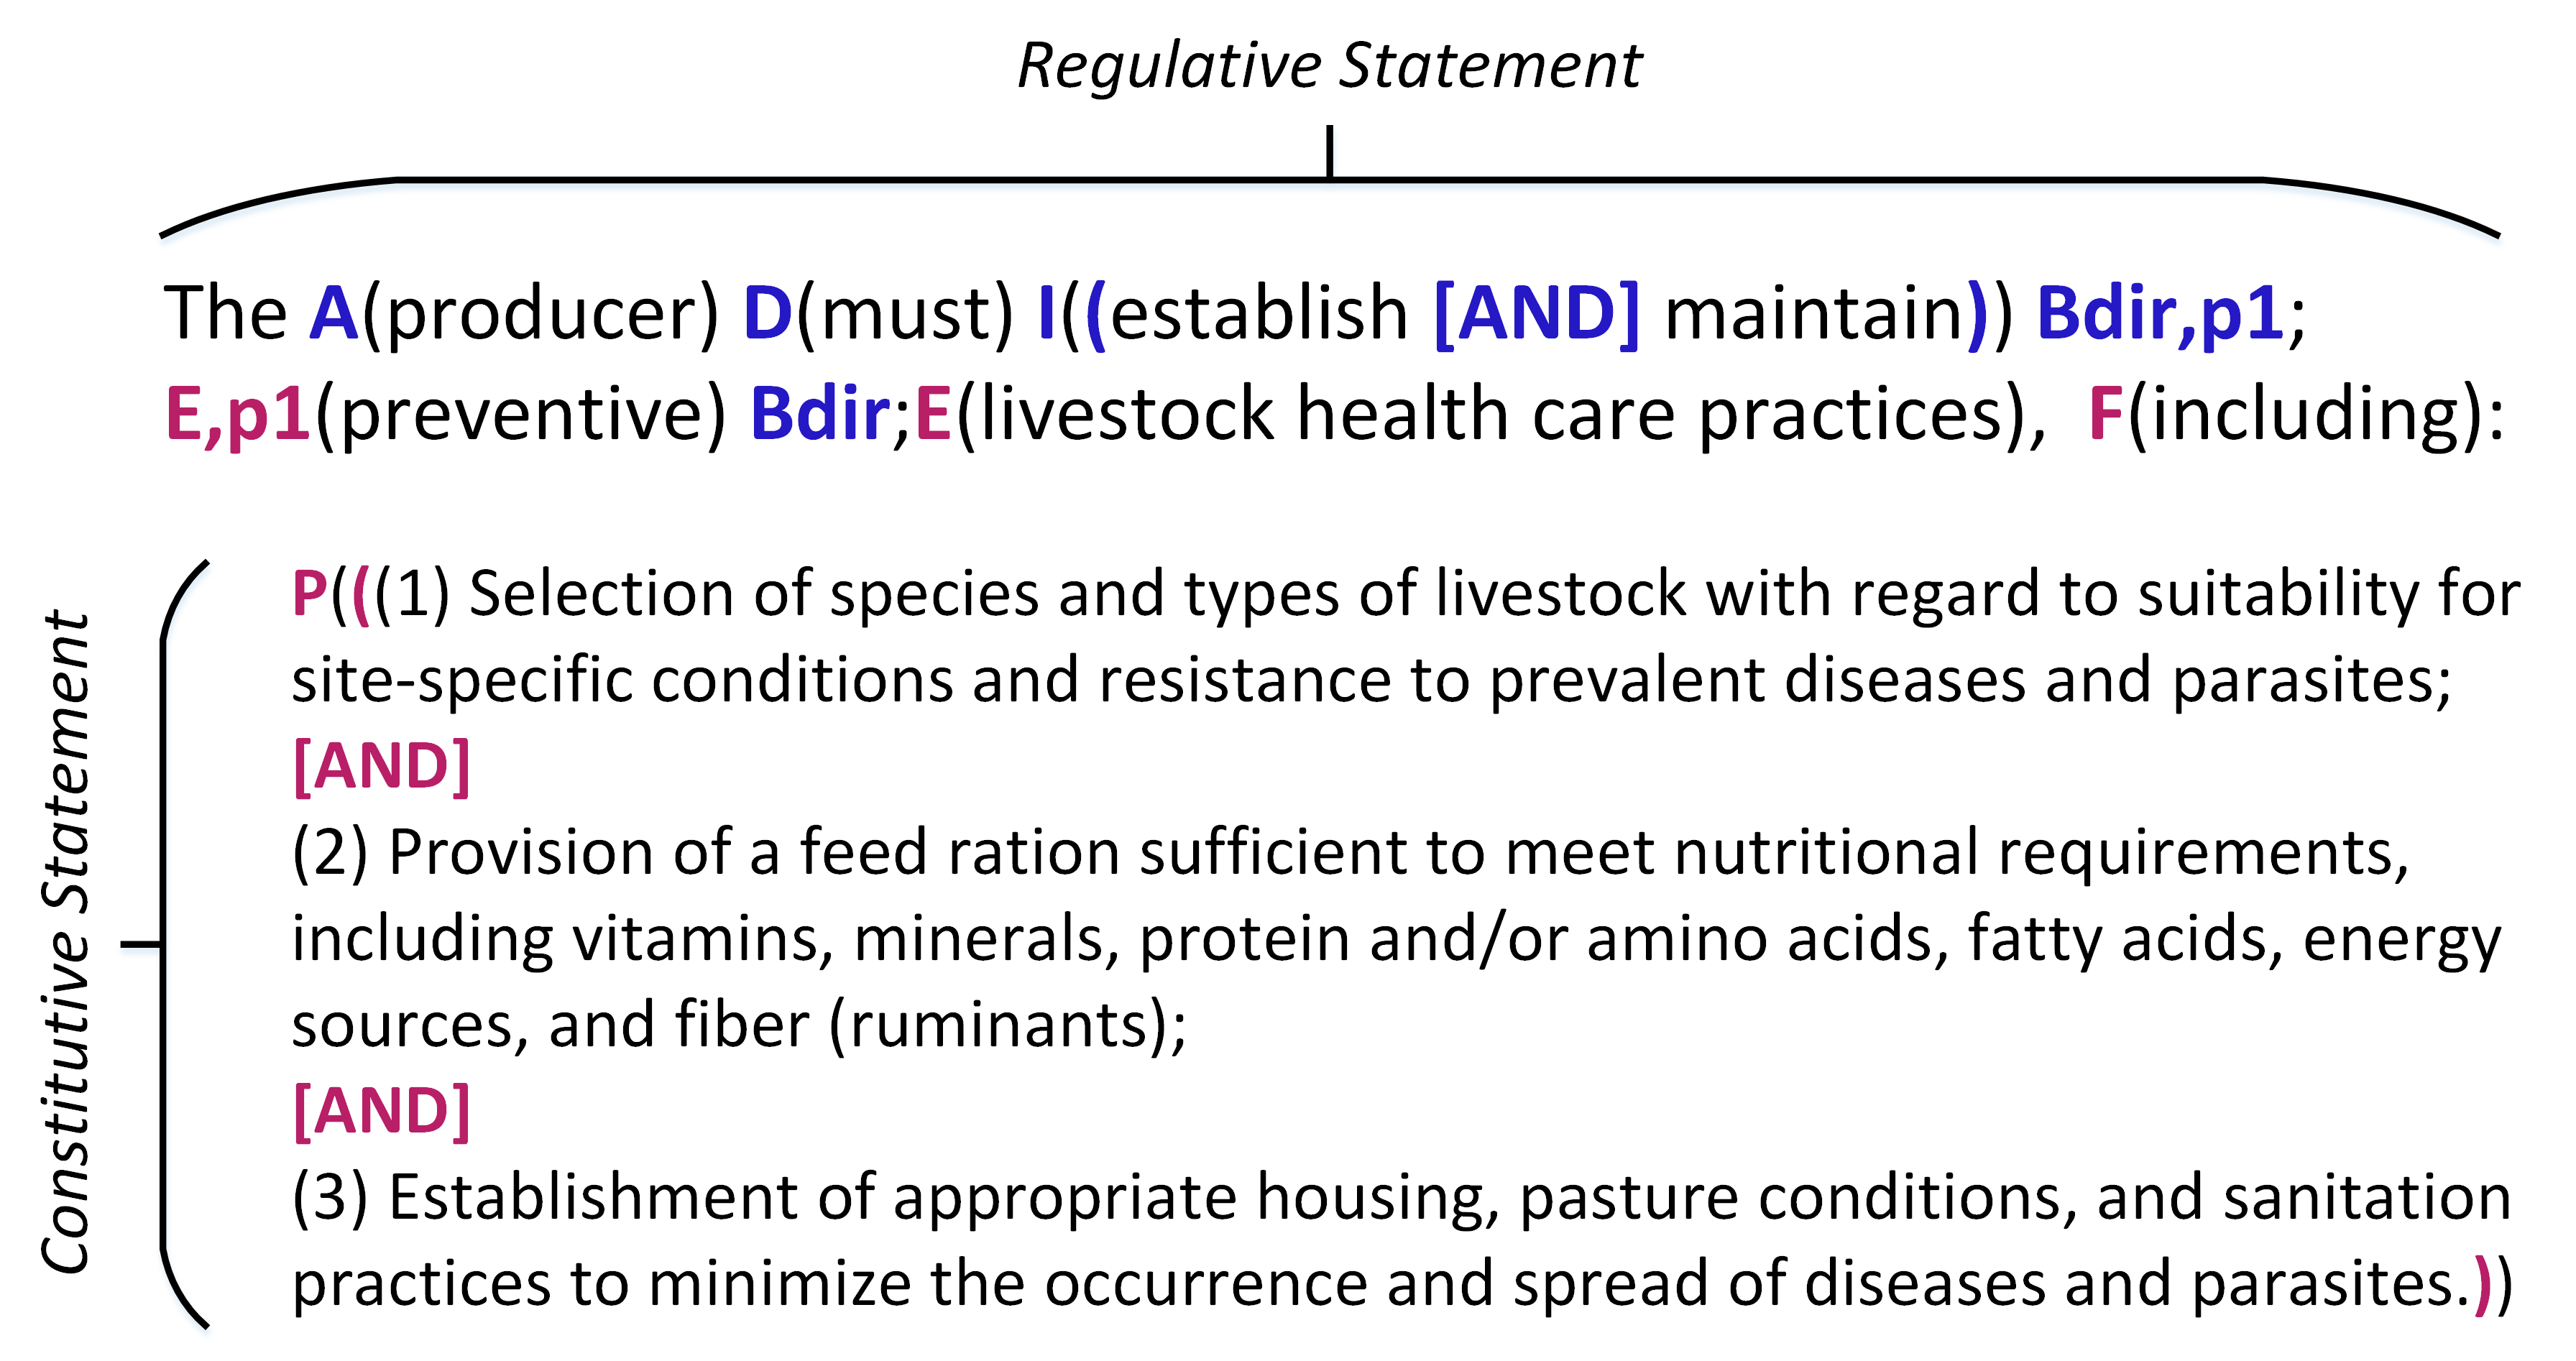
\includegraphics[width=0.8\textwidth]{figures/RegulativeConstitutiveHybridCoded.png}}
    \caption{Coded Regulative-Constitutive Hybrid Example}
    \label{fig:RegulativeConstitutiveHybridCoded}
\end{figure}

In many instances (such as the one shown here), this interleaved representation  affords a decomposition or transformation of hybrids into individual statements by separating the statements by syntactic components, and replication of overlapping components in the individual statements. This decomposition is exemplified in \cref{fig:RegulativeConstitutiveHybridDecomposed}.

\begin{figure}[h!]
    \centering
    \framedfigure{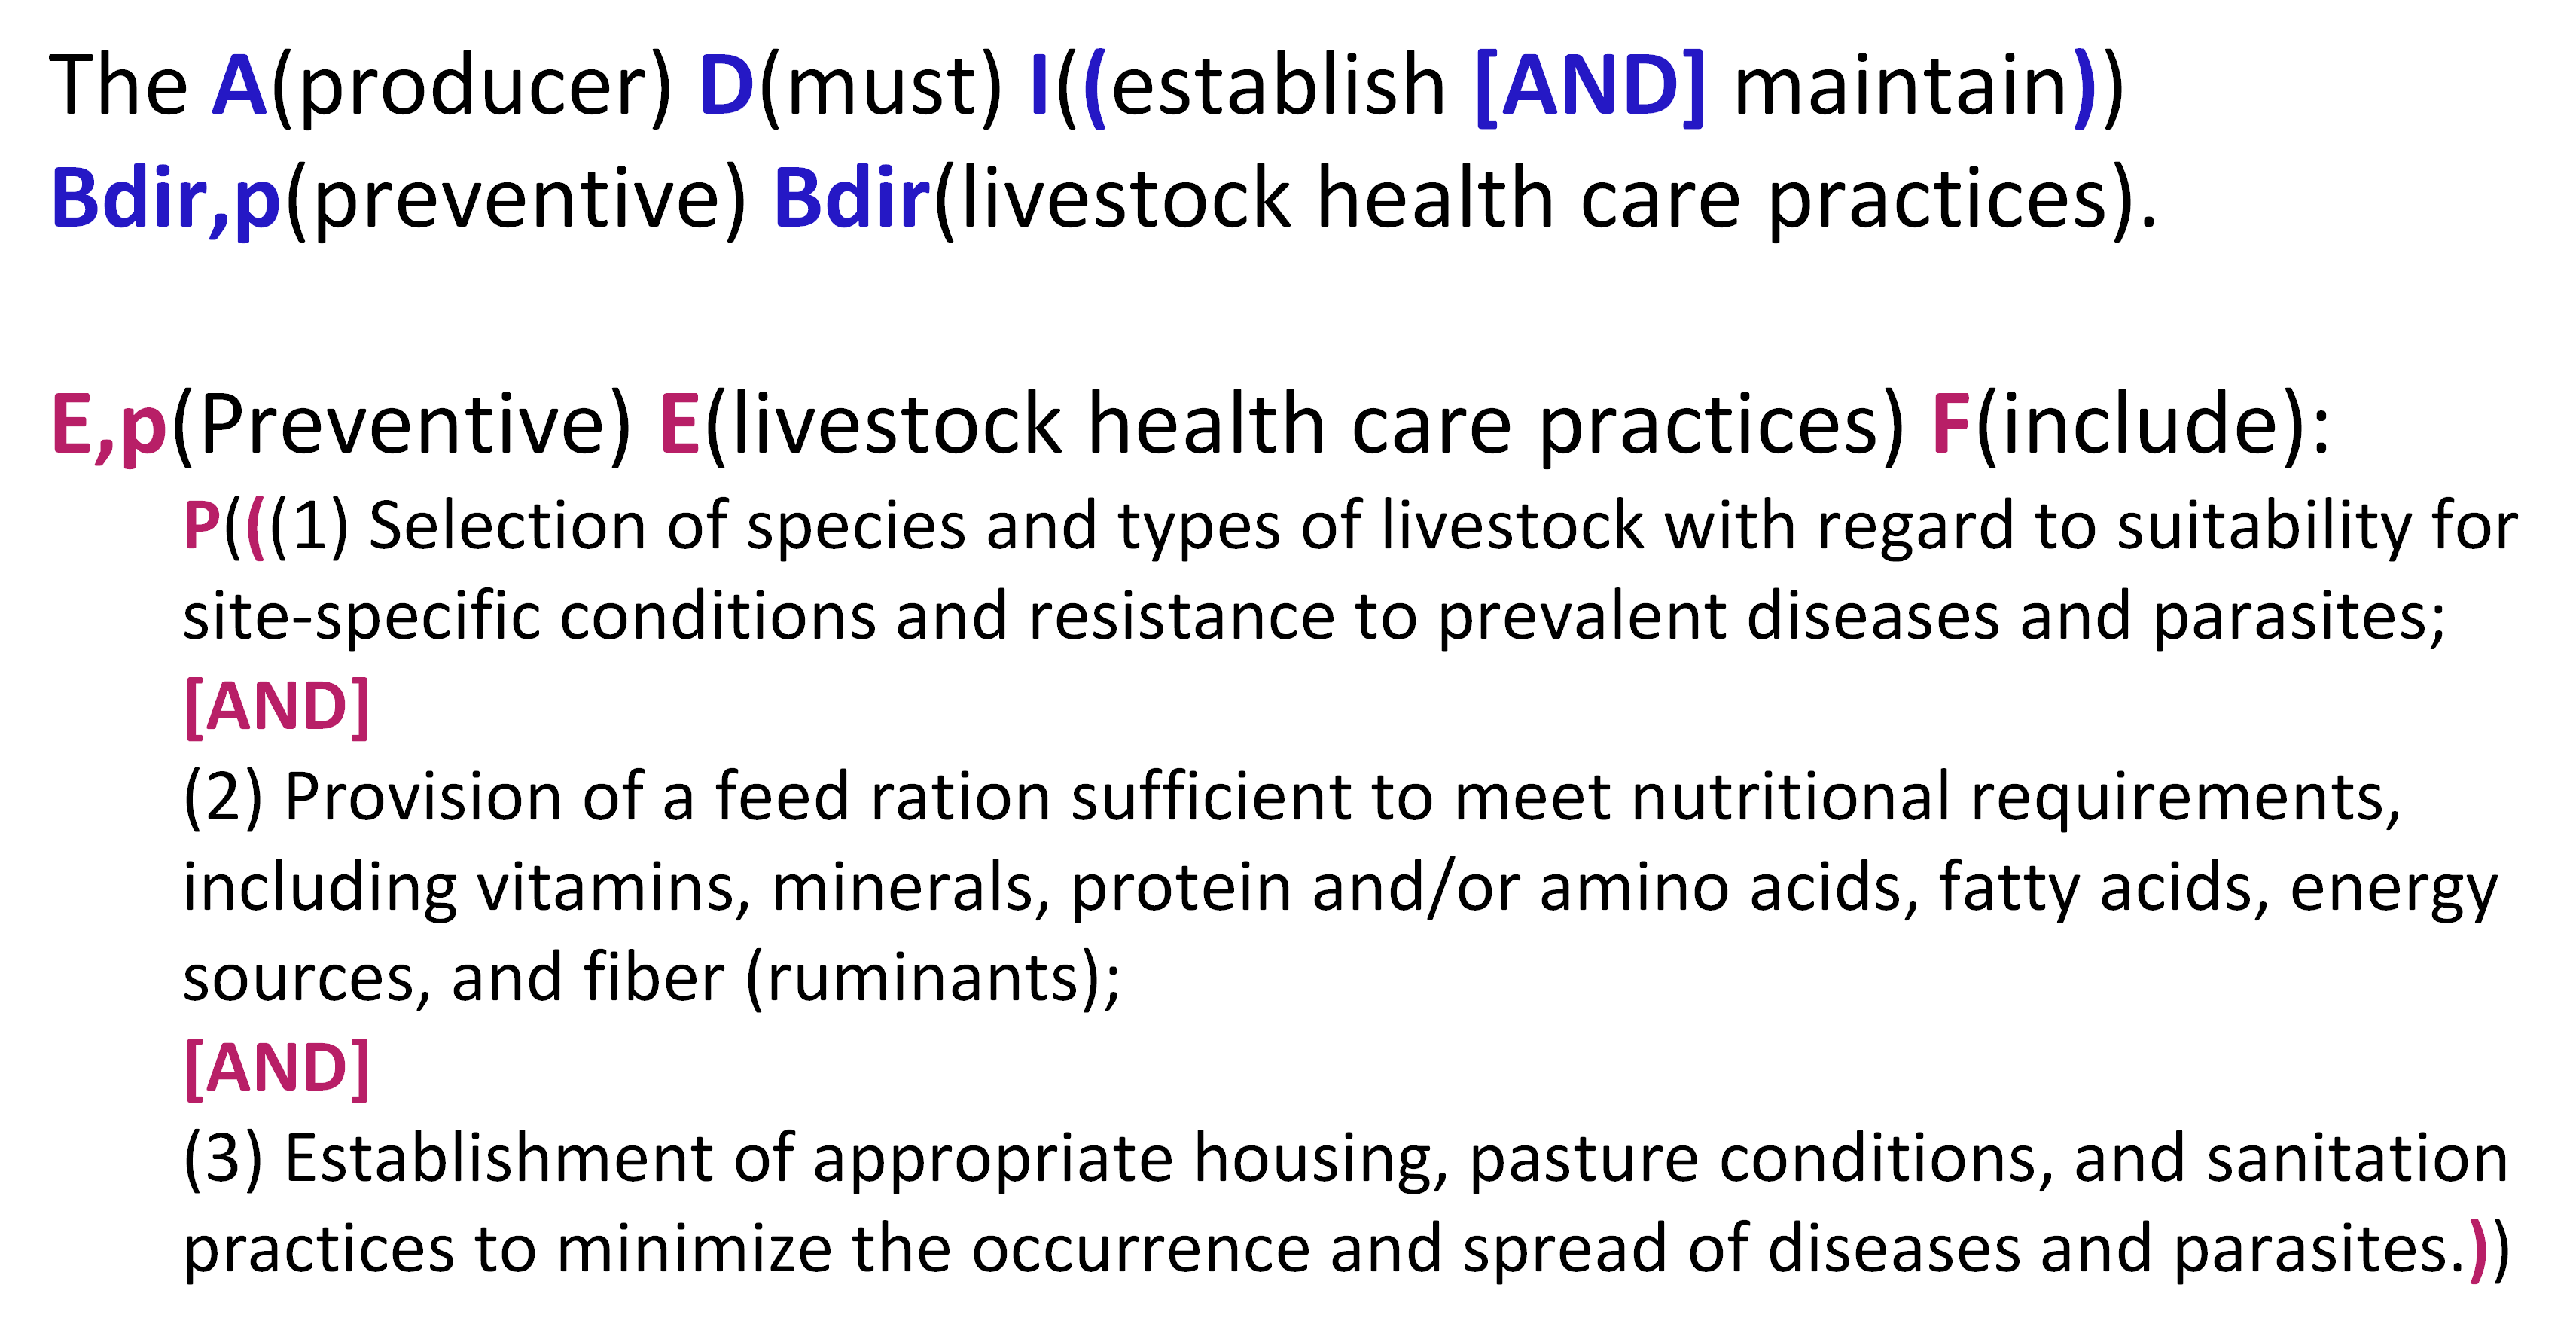
\includegraphics[width=0.8\textwidth]{figures/RegulativeConstitutiveHybridDecomposed.png}}
    \caption{Decomposed Regulative-Constitutive Hybrid Example}
    \label{fig:RegulativeConstitutiveHybridDecomposed}
\end{figure}

 
\newpage

\subsubsection{Constitutive-Regulative Statements}

Contrasting the embedding of constitutive statements in regulative settings, we can likewise observe the embedding of regulative statements in constitutive ones. In the following example (\cref{fig:ConstitutiveRegulativeHybridExample}), the consequence of breaching a constitutive statement\footnote{This statement signals the requirement that diversity is understood as specified.} is expressed in regulative terms, following the principles of statement-level nesting. While the leading statement is coded as a constitutive statement, the consequences are a combination of regulative statements.

\begin{figure}[h!]
    \centering
    \framedfigure{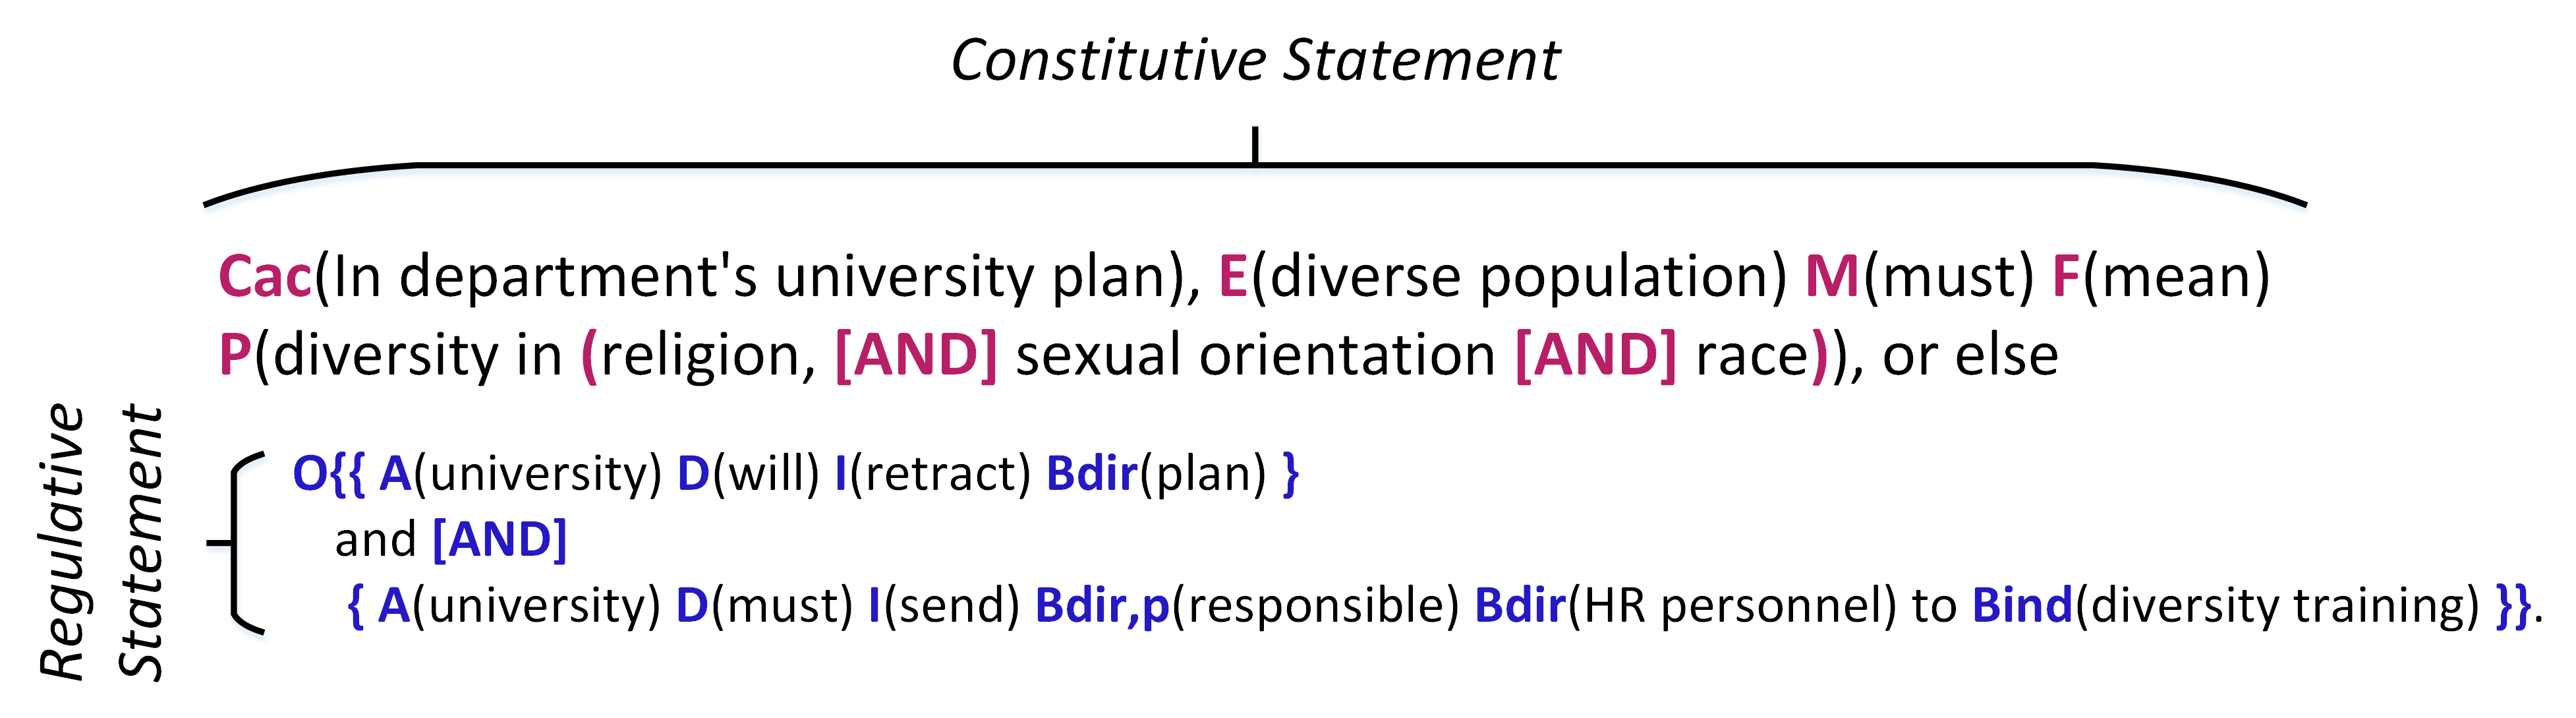
\includegraphics[width=0.9\textwidth]{figures/ConstitutiveRegulativeHybrid.png}}
    \caption{Constitutive-Regulative Hybrid Example}
    \label{fig:ConstitutiveRegulativeHybridExample}
\end{figure}

\subsubsection{Second-Order Constitutive Statements}

In addition to the combined characterisation of constitutive and regulative hybrids, we can further observe component-level nesting of constitutive statements as shown below. While, in principle, equally admissible for regulative statements, specifically the higher-order decomposition of constitutive statements is commonly found. Higher-order decomposition thereby implies the nesting of constitutive statements within individual components, such as property items. Naturally, as motivated in the earlier example, this can occur in conjunction with hybrid statements and independent of the regulative or constitutive nature of the leading institutional statement. 

\begin{figure}[h!]
    \centering
    \framedfigure{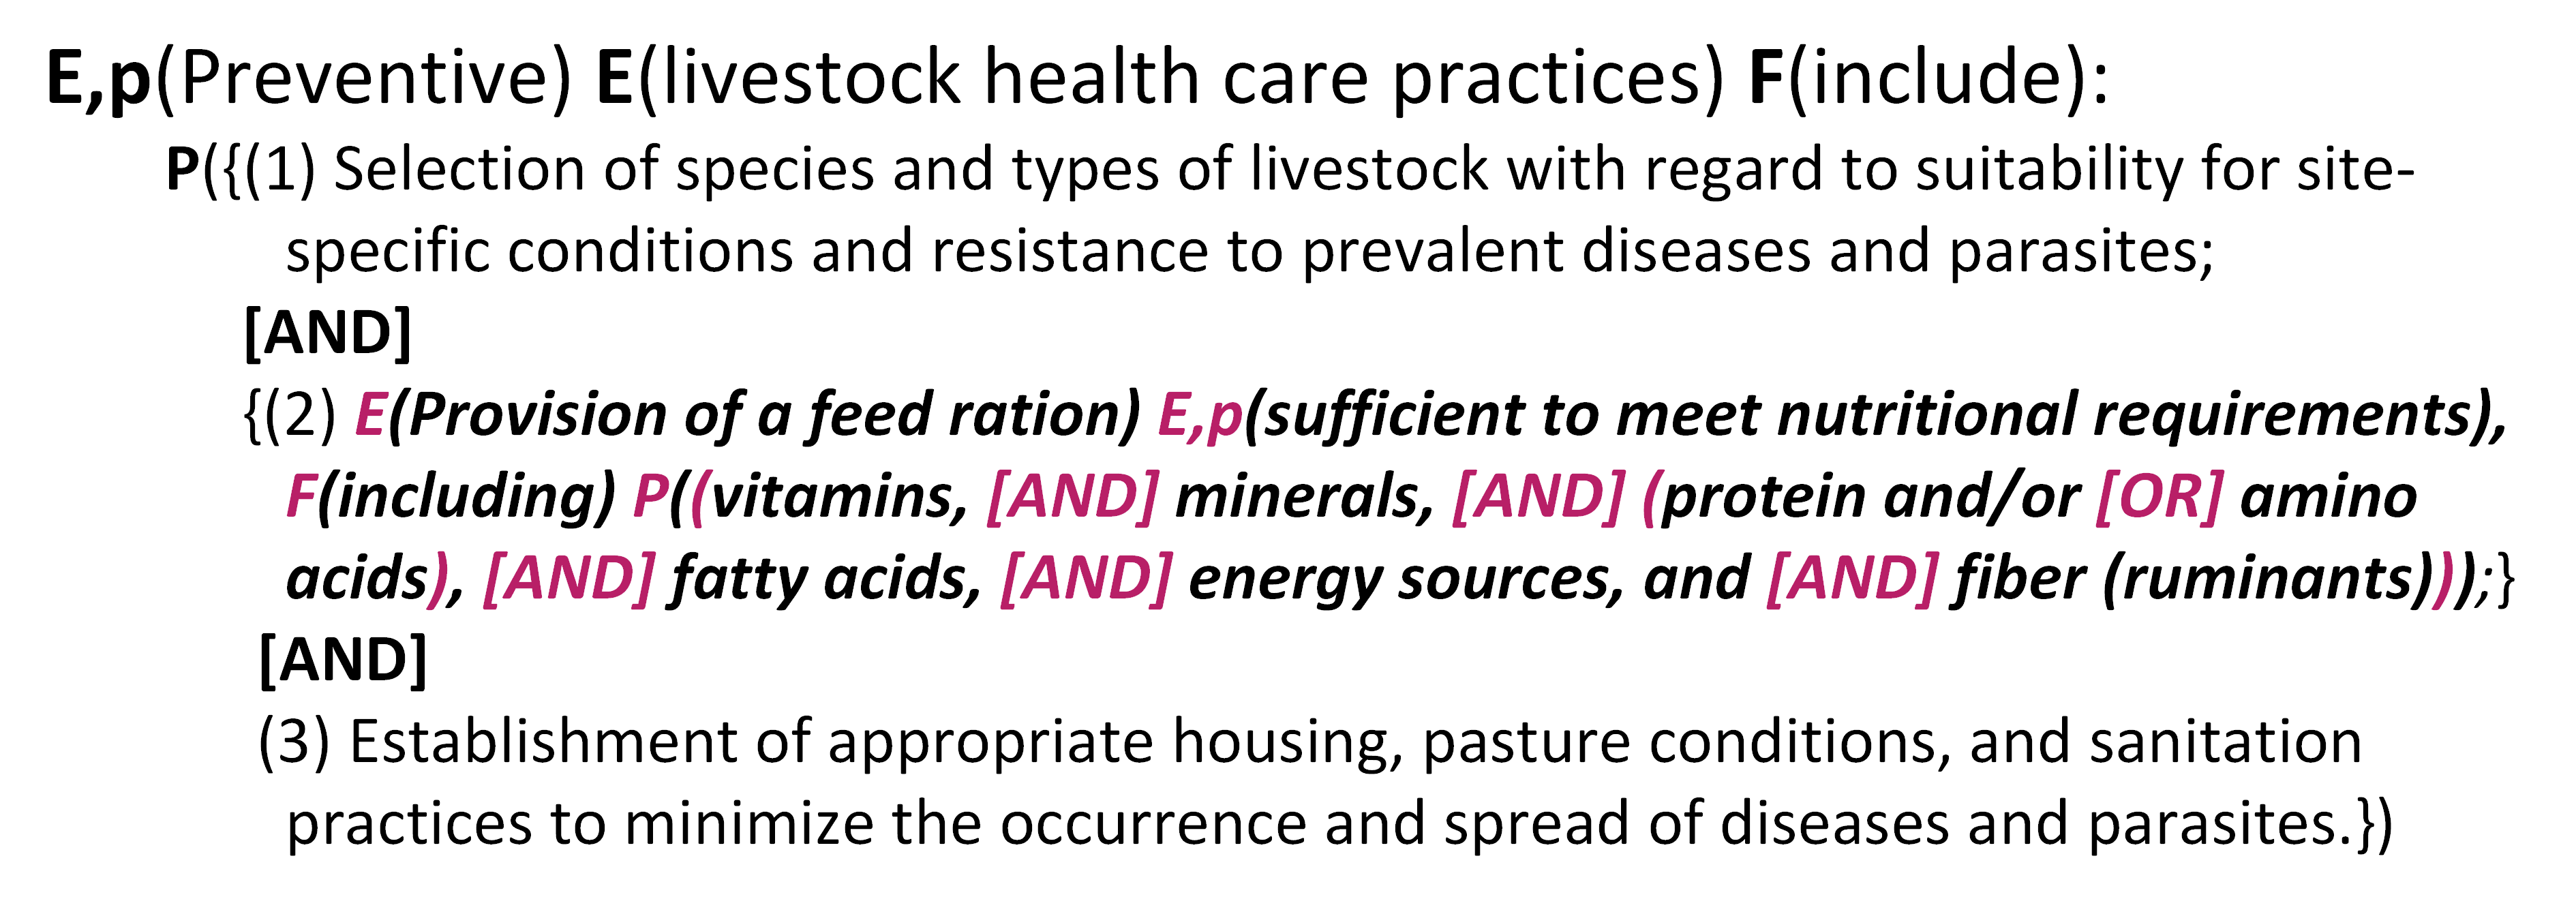
\includegraphics[width=0.8\textwidth]{figures/SecondOrderHybrid.png}}
    \caption{Second-order Constitutive Statement Example}
    \label{fig:SecondOrderHybridExample}
\end{figure}

Reviewing the example above (\cref{fig:SecondOrderHybridExample}, second-order statement in italicized bold font), we note the reference to feed rations as a property element of livestock health care practices that is defined in terms of an embedded constitutive statement that in itself captures a complex set of properties that constitute a feed ration. 

\clearpairofpagestyles
\chead{\headmark}
\automark[subsubsection]{subsubsection}
\ifoot{\ifootertext}
\ofoot{\ofootertext}
\cfoot{\thepage}

\subsubsection{Polymorphic Institutional Statements}
\label{subsec:SyntacticPolymorphs}

Another aspect of discussion of the combined nature of statements relates to the identification of constitutive and regulative statements. The function of either statement type is generally well defined based on the parameterizing role (e.g., introduction or modification of entities or endowment of rights/authority) of constitutive statements, and the behavioral regulation (specification of operational duties and constraints for given actors or actor interaction) captured by regulative statements. While the heuristics provided in \cref{subsec:StatementTypesHeuristics} lend support for an unambiguous characterization of institutional statements as either constitutive or regulative, the characterization may not for all instances be non-contentious, or may make tacit analytical (or coding) preferences overt. While such preferences should inform the coding process by specifying the interpretational scope applied to individual institutional statements (see \cref{subsec:StatementTypesHeuristics}), where the data set is to be encoded in generic form (i.e., without concessions to specific analytical objectives),  %In such cases, or based on given analytical objectives, a specific form of coding (with potential concessions to accurate characterization of statements) may be preferable. 
%
%Possible reasons for and approaches to resolve this ambiguity include the nature of the policy more generally, i.e., in how far the specific statement regulates central concerns of the policy, as opposed to parameterizing the scenario, or contextualizing the policy itself. Other, more specific indicators include the positioning of the statement within the document. If located in the preamble, for example, the intended interpretation as constitutive statement is likely. Another consideration is the immediate context of a statement, i.e., its surrounding statements. Those may offer a clearer indication as to whether the statement is of configurational nature (constitutive), or bears operational weight (regulative). A further heuristic is of stylistic nature. Reviewing the coded document, the coder may find specific terms characteristic for constitutive or regulative statements in the context of the policy and/or field (e.g., the use of ``shall'' as indicative for constitutive statements, if obligations in regulative statements are commonly expressed using more distinctive and specific deontics). 
%
%Where such is the case, statements can be cod using both syntactic forms, and identifying in how far the encoding affords extensive reformulation or reconstruction of a statement in order to arrive at a sensible coding outcome. 
%
%As an alternative to the focus on statement purpose, analytical objectives may drive a preference for either statement type in the form of a default strategy for the treatment of ambiguous statement types. 
%If, for example, the understanding of actor relationships across a given policy is of fundamental concern, but reconstruction of configurational aspects external to actorship are secondary, a potential default strategy for the coding of ambiguous statements (e.g., defined as part of the project-specific guidelines) could be their interpretation as regulative. 
%
%Where ambiguous expression, and in consequence, flexibility exists, 
statements can be considered \begin{emp}polymorphic institutional statements\end{emp}, or \begin{emp}syntactic polymorphs\end{emp}. This means, they are encoded in both forms, and the analyst can draw on either shape depending on their desired analytical use. 

To substantiate this approach with an example, let us use the statement \begin{exa}``The functions of the Board shall be: (a) give effect to the decisions and policies of the Health Assembly; (b) perform any other functions entrusted to it by the Health Assembly.''\end{exa}

This statement can be read in constitutive terms, since it parameterizes the institutional system with respect to a specific entity, namely the characterization of the board in terms of its assigned functions and endowed responsibilities. The statement, however, can also be read in regulative terms, in which the functions of the board are expressed as obligations (and thus as regulated behavior) in operational terms. The same statement can thus be encoded as a polymorph by drawing on syntactic components of both statement types, as visualized in the following (including color coding to signal regulative (\textcolor{\corecolor}{\corecolorname}) and constitutive components (\textcolor{\corecolorconst}{\corecolorconstname}), respectively).

\sp

\fcolorbox{black}{\boxbgcolor}{\begin{minipage}{16.0cm}

\begin{exa}
The \E{}(functions) of the \A{}(Board) \D{}/\M{}(shall) \F{}(be): 

\Pp{}\lp \{

\hspace{0.2cm} (a) \I{}(give) \Bdir{}(effect) to the \Bind{}(decisions) of the \Bind{},\prop{}(Health Assembly); 

\hspace{0.2cm} \AND

\hspace{0.2cm} (b) \I{}(perform) \Bdir{}(any other functions)  \Bdir{},\prop{}(entrusted to it by the Health Assembly)

\hspace{0.1cm} \}\rp.
\end{exa}

\end{minipage}}

\sp

The coding shows overlap, but the central components for regulative and constitutive statements (namely constituted entity, attributes, constitutive function, aim, as well as constituting properties) showcase the varying focal aspects of different statement types. Subject to emphasis on either the actor (i.e., `the Board') or its functions (i.e., `the functions') can determine the coding, or even admit both approaches for analytical purposes.

A specific value of the polymorphic representation is to make the linkage between configurational aspects that affect the wider institutional setting, and behavioral regulation that specifically embeds actors in this institutional setting, both configurationally, as well as operationally, explicit.

While the notion of polymorphic structure is explicit in the previous example, the coding of statements in both forms can be more complex and may even afford reconstruction, as shown in the following example, with the same statement coded separately in constitutive and regulative forms: \begin{exi}``Members of the Council shall have the right to hold any public office or employment.''\end{exi}

In constitutive terms the statement reflects the Council members endowment with a right, namely the right to hold other public positions in addition to a Council membership, and is encoded as follows: 

\sp

\fcolorbox{black}{\boxbgcolor}{\begin{minipage}{15.5cm}
\begin{exi}\E{}(Members) of the \E{},\propconst{}(Council) \M{}(shall)  \F{}(have the right) \Pp{}(to hold any other public office or employment).\end{exi}
\end{minipage}}

\sp

Here, the Council member is at the center of the encoding. Depending on the analytical use (e.g., assumed actor perspective), constitutive statements reflect an abstract conception of a right or a property. Expressing this assurance in regulative terms by invoking the principle of \begin{emp}jural correlatives\end{emp}~\citep{Hohfeld1913SomeReasoning} requires the representation of behavioral constraints by introducing a conception of actorship in the form of a tacit (and in this case unidentified) actor whose behavior is regulated as corresponding duty, alongside further structural adaptations. Reconstructing the statement in regulative terms\footnote{Explicit transformation rules associated with the reconstruction of statements of various types are subject to forthcoming work.} thus produces the following coding:\footnote{Note that the following coded samples call out negations of deontics and modals explicitly for clarity.}

\sp

\fcolorbox{black}{\boxbgcolor}{\begin{minipage}{15.5cm}
\begin{exi}\A{}([Attribute])~\D{}([must]) \NOT{}~\I{}(disqualify)  \Bdir{}(member of the council) \Cex{}(from holding any other public office or employment).\end{exi}
\end{minipage}}

\sp

Exemplifying the use of polymorphic structures and their practical implications further, the following statement constellation highlights interpretational challenges associated with statement references. 

Assessing the set of statements shown below, we specifically turn our attention to the final statement. This statement is embedded within a paragraph of statements that regulate operational activity, but this statement specifically introduces further constraints that apply to all other statements. 

Encoding this statement using a \begin{emp}narrow interpretational scope\end{emp} (as described in \cref{subsec:StatementTypesHeuristics}), the statement can be interpreted as parameterizing the wider institutional setting by affecting a series of provisions (``Paragraphs in this section'') and furthermore clearly signaling the requirement that the paragraphs do not apply (see \begin{emp}Deontic vs.~Epistemic Modal\end{emp} heuristic in \cref{tab:SemanticStatementTypeHeuristics} in \cref{subsec:StatementTypesHeuristics}). Consequently, the statement is coded as constitutive (as exemplified below). 

\sp
\fcolorbox{black}{\boxbgcolor}{\begin{minipage}{15.5cm}
\begin{exi}
(1) Organic farming operations must not utilize genetically-modified seeds.

(2) Organic farming operations may not process crops other than the ones specified in Appendix A.

\dots

(10) \E{}(Paragraphs in this section) \M{}(do) \NOTconst{}~\F{}(apply) \Pp{}(to traces) \Pp{},\propconst{}(of genetically modified material).
\end{exi}
\end{minipage}}
\sp

However, given the evident regulative nature of the referenced statements, coding such statement with \begin{emp}wide interpretational scope\end{emp} in mind leads to a resolution of the semantic links to the referenced statements, and doing so, affords a reconstruction of the statement in regulative form -- rendering the following encoding (simplified for illustrative purposes):

\sp
\fcolorbox{black}{\boxbgcolor}{\begin{minipage}{15.5cm}
\begin{exi}
\A{}(Organic handling operations) \D{}(may) \NOTconst{}~\I{}(apply)  \Bdir{}(paragraphs in this section) to \Bind{}(traces) \Bind{},\prop{}(of genetically modified material).
\end{exi}
\end{minipage}}
\sp

Similar to the previous case, the coding requires reformulation of the statement in regulative terms. However, unlike the previous case, the specification of the responsible actor is explicit in the referenced institutional statements, thus affording a reliable encoding in a form that is aligned with the syntactic structure of the related institutional statements. As indicated for all cases above, the coding of such statement can selectively take regulative and constitutive form where interpretational scope favors narrow and wide resolution of semantic linkages. As showcased for the first example, where coding is independent from analytical use, the statement can be concurrently encoded in both forms. 

\udl{Note:} As discussed in the context of the interpretational scope applied by the coder (see \cref{subsec:StatementTypesHeuristics}), encoding statements in constitutive and/or regulative forms may invoke varying levels of complexity with respect to necessary adaptations of the statements, and, depending on analytical objectives, potential modifications of the statement semantics (in the given example, a concrete actorship for regulative statements is presumed, whereas the right more generally is expressed in constitutive terms). This can require a reformulation that could be challenged on methodological grounds and thus considered during design of the study. In addition to considering a dual annotation in the first place, the potential mischaracterization of a statement as either regulative or constitutive may be sensibly assessed in small-scale inter-coder reliability tests to resolve disagreements and misconceptions early in the encoding process.

\newpage

\subsection{Data Structure Patterns}
\label{subsec:DataStructurePatterns}

\begin{emp}Note that this section is under ongoing development and will likely experience significant extension in upcoming releases.\end{emp}

\vspace{0.5cm}

Another aspect related to the features introduced for both regulative and constitutive statements is the recognition of data structure patterns. A pattern commonly observed is the notion of collections, such as composition of committees, definition of practices in terms of underlying activities, delineation of goals or outcomes to be pursued, etc.

\sp 

\udl{Collections:} While dominant in objects and constituting properties, respectively, those can occur across other components (e.g., context). Central here is the identification of a collection descriptor and the corresponding elements, along with the explicit specification of logical operators that link the individual elements.

\sp

Example: \begin{exi}\E{}(Health care practices) \F{}(consist of) \Pp{}(\lpconst preventative measures [\ANDconst] appropriate nutrition [\ANDconst] rest\rpconst)\end{exi}. 

\sp

\udl{Complex elements:} Where quantitative information is expressed, or listed (and thus potentially embedded in collections or referred to as a single item), the elements commonly follow a schematic structure specific to individual documents (e.g., based on style or disciplinary background), but follow general patterns, such as variations of the following: \begin{exi}\textbf{[qualifier] [comparator] [quantity] [unit] [object property] [object]}\end{exi}. 

\sp

Example: \begin{exi}significantly (qualifier) more than (comparator) 10 (quantity) tons (unit) high-quality (object property) building material (object)\end{exi}

\sp

While those patterns can vary in extent and detail, their consideration in project-specific coding guidelines can be useful in as far as they are relevant for analytical purposes.

\sp

\udl{Comparisons/Equations:} In many instances, statements, and more specifically, activation conditions, are expressed in terms of comparisons, such as ``if gender distribution within department staff substantially differs from distribution within the wider organization, \dots''. Comparisons of such kind can be expressed in equation form, following the general pattern \textbf{[left-hand side] [comparison operator] [right-hand side]}, where left- and right-hand sides can be of simple form (e.g., numeric) or complex (e.g., consisting of complex elements as introduced above). Comparison operators include the following: $<$, $\leq$, $\lesssim$, $\approx$, $=$, $\gtrsim$, $\geq$, $>$, amongst others such as $\neq$. Oftentimes, comparators can further be complemented by additional qualification of the relationships. 

\sp

Example: \begin{exi}if gender distribution (object) within department staff (object property) substantially (qualifier) differs ($\neq$) from distribution (object) within the wider organization (object property)\end{exi}

\sp

Naturally, generic mathematical expressions are likewise conceivable, but not subject to further elaboration at this stage. Where coding on finer levels of granularity (e.g., resolving comparative relationships) is relevant, level and specific form of decomposition should be considered as part of the study design.
\newpage

% Header reference level
\clearpairofpagestyles
\chead{\headmark}
\automark[subsection]{subsection}
\ifoot{\ifootertext}
\ofoot{\ofootertext}
\cfoot{\thepage}


\subsection{IG Configurations (Institutional Grammar Profiles)}
\label{subsec:IgProfiles}

As discussed before, the various coding levels of IG 2.0 accommodate different analytical needs as well as complexity of the encoded documents. Commitment to a level, including all the associated features, may in some cases be too coarse-grained to accommodate analytical needs. This can include, for example, the omission of components entirely, as well as the selective considerations of features of higher coding levels. To capture the considered feature set, a coded dataset should be accompanied with the applied coding configuration. 

For this purpose, we specify a fine-grained configuration syntax that allows the choice of features across levels of IG 2.0. The features for individual levels as specified in this document are captured in \cref{tab:IGProfilesRegulative} for regulative statements, and \cref{tab:IGProfilesConstitutive} for constitutive statements, along with a symbol specification used for the definition of specific IG configurations, or profiles.


\begin{table}[h!]
\centering
\begin{threeparttable}
\begin{tabular}{p{3cm} p{9cm} p{2cm}}
\toprule
\textbf{Coding Level} & \textbf{Feature} & \textbf{Symbol} \\
\toprule
IG Core & \multicolumn{1}{p{10em}}{Attributes} & A \\
IG Core & \multicolumn{1}{p{10em}}{Object\tnote{1}} & B \\
IG Core & \multicolumn{1}{p{10em}}{Deontic} & D \\
IG Core & \multicolumn{1}{p{10em}}{Aim} & I \\
IG Core & \multicolumn{1}{p{10em}}{Context\tnote{2}} & C \\
IG Core & \multicolumn{1}{p{10em}}{Or else} & O \\
\midrule
IG Extended & \multicolumn{1}{p{10em}}{Attributes refinements} & A$\subtxtNormal{Ext}$ \\
IG Extended & \multicolumn{1}{p{10em}}{Object refinements\tnote{1}} & B$\subtxtNormal{Ext}$ \\
IG Extended & \multicolumn{1}{p{10em}}{Context refinements\tnote{2}} & C$\subtxtNormal{Ext}$ \\
\midrule
IG Logico & Statement references & R \\
IG Logico & Logical relationship annotations & L \\
IG Logico & Semantic annotations & S \\
IG Logico & Regulative function annotations\tnote{3} & \Ureg \\
\toprule
\end{tabular}

\begin{tablenotes}
\footnotesize
\item[1] Where the configuration is specific to direct or indirect object component, those can be indicated using \Bdirraw~and \Bindraw, respectively; where applied in combination with the specification of IG Extended features, `$\subtxtNormal{,Ext}$' is appended accordingly (e.g., \Bdirraw$\subtxtNormal{,Ext}$).
\item[2] Where the configuration is specific to activation condition or execution constraint component, this can be indicated using \Cacraw~and \Cexraw, respectively; where applied in combination with the specification of IG Extended features, `$\subtxtNormal{,Ext}$' is appended accordingly (e.g., \Cacraw$\subtxtNormal{,Ext}$).
\item[3] Where institutional functions are annotated for both regulative and constitutive statements, the symbol U (without subscript) is used.
\end{tablenotes}
\end{threeparttable}

\caption{IG Feature Specifications for Regulative Statements}
\label{tab:IGProfilesRegulative}
\end{table}

\begin{table}[h!]
\centering

\begin{threeparttable}
\begin{tabular}{p{3cm} p{9cm} p{2cm}}
\toprule
\textbf{Coding Level} & \textbf{Feature} & \textbf{Symbol} \\
\toprule
IG Core & Constituting Properties & P \\
IG Core & Modal & M \\
IG Core & Constituted Entity & E \\
IG Core & Constitutive Function & F \\
IG Core & Context\tnote{1} & C \\
IG Core & Or else & O \\
\midrule
IG Extended & Constituting Properties refinements & P$\subtxtNormal{Ext}$ \\
IG Extended & Constituted Entity refinements & E$\subtxtNormal{Ext}$ \\
IG Extended & Context refinements\tnote{1} & C$\subtxtNormal{Ext}$ \\
\midrule
IG Logico & Statement references & R \\
IG Logico & Logical relationship annotations & L \\
IG Logico & Semantic annotations & S \\
IG Logico & Constitutive function annotations\tnote{2} & \Ucon \\
\toprule
\end{tabular}

\begin{tablenotes}
\footnotesize
\item[1] Where the configuration is specific to activation condition or execution constraint component, this can be indicated using \Cacraw~and \Cexraw, respectively; where applied in combination with the specification of IG Extended features, `$\subtxtNormal{,Ext}$' is appended accordingly (e.g., \Cacraw$\subtxtNormal{,Ext}$).
\item[2] Where institutional functions are annotated for both regulative and constitutive statements, the symbol U (without subscript) is used.
\end{tablenotes}
\end{threeparttable}

\caption{IG Feature Specifications for Constitutive Statements}
\label{tab:IGProfilesConstitutive}
\end{table}


Using coding levels, along with \textbf{--} and \textbf{+} symbols in combination with specific features references as listed in the table, we can express specific coding configurations, or coding profiles, that allow the omission or inclusion of features across all levels, or the selective coding of specific components based on lower coding levels.

Abstractly specified, a configuration has the following structure (where $<$ and $>$ embeds symbol characterizing features omitted from or added to the baseline coding level): 

\sp

{\small
\begin{emp}\textbf{$<$Baseline level$>$--$<$omitted features from baseline level$>$+$<$additional features from higher level$>$}\end{emp}}

\sp

\noindent\udl{Examples:} To capture the commitment to IG Core, along with the Context coding from IG Extended (e.g., component-level nesting, use of taxonomies, is specified as the configuration \begin{emp}\textbf{IG Core+C$\subtxtNormal{Ext}$}\end{emp}, where the \begin{emp}\textbf{+C$\subtxtNormal{Ext}$}\end{emp} signals features from the next higher level (IG Extended). 

Conversely, we can specify coding on IG Core level as the baseline, but without the consideration of Or else components as \begin{emp}\textbf{IG Core--O}\end{emp}. Where multiple components are omitted, we can specify \begin{emp}\textbf{IG Core--IO}\end{emp}, where features should be referred to in the order specified in the table (here: \begin{emp}Aim\end{emp} before \begin{emp}Or else\end{emp}). Selectively capturing features from IG Logico in IG Core-based coding, \begin{emp}\textbf{IG Core+R}\end{emp} indicates the coding of statement relationships in addition to the base IG Core coding.

Finally, omission and extensions can be combined, with omissions specified first, followed by feature additions, such as \begin{emp}\textbf{IG Extended-B\Cexraw+S\Ureg}\end{emp}, to signal the coding of Object and execution constraints on IG Core level, while considering semantic annotations and institutional functions (here for regulative statements only) in addition to this (reduced) IG Extended baseline. Complementing this discussion for the highest level, \begin{emp}\textbf{IG Logico-S}\end{emp} would imply complete coding on IG Logico level under omission of semantic annotations only.

Combining both omission and extension leverages complete flexibility with respect to the composition of features, and, where analytically useful, in principle even foregoing the inclusion of components defined necessary for institutional statements (i.e., A, I, and C component for regulative statements; F, E, and C for constitutive statements). For example, modeling the selective omission of components entirely, along with the inclusion of advanced features, \begin{emp}\textbf{IG Core-AI+C$\subtxtNormal{Ext}$SU}\end{emp} signals IG Core baseline encoding under omission of Attributes and Aim, while adding refined coding of Context (based on IG Extended), along with features from IG Logico, namely semantic annotations and institutional functions (here both for regulative and constitutive statements).

A common encoding level that offers the smallest possible extension to previous coding practice of institutional statements based on Crawford and Ostrom's original grammar is \begin{emp}\textbf{IG Core+C$\subtxtNormal{Ext}$}\end{emp}.

\noindent\udl{Custom refinements:} Where coders seek more fine-granular refinements (e.g., applying a subset of the features of a given configuration (e.g., coding objects without properties), such modifications should be indicated alongside the specified configuration. Similarly, extensions (e.g., additional taxonomies, or extensions or substitution of existing ones) should be documented alongside the configuration.

